\documentclass[titlepage,a4paper]{article}

\usepackage{a4wide}
\usepackage[colorlinks=true,linkcolor=black,urlcolor=blue,bookmarksopen=true]{hyperref}
\usepackage{bookmark}
\usepackage{fancyhdr}
\usepackage[spanish]{babel}
\usepackage[utf8]{inputenc}
\usepackage[T1]{fontenc}
\usepackage{graphicx}
\usepackage{float}

\usepackage{amssymb} % simbolos matematicos

\usepackage{minted} % codigo
\usepackage[table,xcdraw]{xcolor} % para los colores en las tablas


\pagestyle{fancy} % Encabezado y pie de página
\fancyhf{}
\fancyhead[L]{Apuntes de BDD - BG}
\fancyhead[R]{2C2021}
\renewcommand{\headrulewidth}{0.4pt}
\fancyfoot[C]{\thepage}
\renewcommand{\footrulewidth}{0.4pt}

\begin{document}
\begin{titlepage} % Carátula
	\hfill
\includegraphics[width=6cm]{logofiuba.jpg}
    \centering
    \vfill
    \Huge \textbf{Apuntes de Bases de datos}
    \vskip2cm
    \Large [7515] Base de Datos\\
    2C 2021
    \vfill
    \begin{tabular}{ | l | } % Datos del alumno
      \hline
      Grassano, Bruno \\ \hline
      bgrassano@fi.uba.ar \\ \hline
  	\end{tabular}
    \vfill
    \vfill
\end{titlepage}

\tableofcontents % Índice general

\newpage

\section*{Introducción}\label{sec:intro}
El presente archivo contiene los apuntes que fueron tomados a lo largo de la cursada de la materia Base de Datos (75.15).

La materia esta muy buena, sin embargo hay que tener en cuenta que es pesada debido a la gran cantidad de temas que abarca. 

Muy recomendable ir siguiendo la materia al día e ir haciendo los parcialitos (fueron 6 este cuatri) para llegar bien al parcial. Después para el final también recomiendo seguirla al día, ya que se puede evaluar cualquier tema de los vistos (ya sea teórico o practico)

\newpage
\section*{Clase 1}
\section{Introducción a bases de datos}

Palabras clave: lugar, datos, persistente, datos interrelacionados (que provienen de un cierto universo en común, tienen relaciones)

\noindent\rule{\textwidth}{0.5pt}

Definición: Una base de datos es un conjunto de datos interrelacionados.

\medskip

Definición: Un dato es un hecho que puede ser representado y almacenado de alguna forma, y que tiene un sentido implícito. 
Lo puedo codificar de alguna forma, no es algo abstracto

\noindent\rule{\textwidth}{0.5pt}


\section{Bases de datos tradicionales vs. no tradicionales}

\noindent\rule{\textwidth}{0.5pt}

Definición: El predicado es una función que toma uno o mas argumentos y devuelve un valor de verdad.

\noindent\rule{\textwidth}{0.5pt}

\subsubsection*{Ejemplos}
\begin{itemize}
\item La mesa 5 consumió 2 milanesas napolitanas y 1 botella de vino
\item 100 gramos de chocolote poseen 546 calorias
\end{itemize}

\smallskip

Todas las oraciones van a tener un sujeto, verbo y predicado.

\smallskip

Las bases de datos almacenan proposiciones
\begin{itemize}
\item Juan gano x en 2012
\item Martin gano x en 2015
\end{itemize}

Todas tienen la misma estructura, se pueden tipificar en un predicado al tener la misma estructura. Podemos separar el nombre, el x, y el año.

Puedo definir una función, que tome como variable las cosas en común que identificamos antes y devuelva Verdadero o Falso de acuerdo a la entrada. Las bases de datos solo almacenan proposiciones verdaderas. Toma determinados predicados, y guarda aquellos que son verdaderos. Estas son las bases de datos \textbf{tradicionales}.

\smallskip

Actualmente las bases de datos pueden almacenar datos mas complejos ahora. \textit{Imágenes, audio, vídeos, etc} Estas son del tipo base de datos \textbf{no tradicional}.

\medskip

\textit{Lectura recomendada: \href{https://www.dcs.warwick.ac.uk/~hugh/M359/What-a-Database-Really-Is.pdf}{What a database really is: Predicates and propositions}}


\section{Sistemas de gestión de bases de datos}
Surge para evitar tener que rehacer los programas cada vez que cambiaba la base de datos. Se hizo evidente que la relación directa entre los programas y los datos es una gran desventaja. Por lo que aparece el gestor como punto intermedio

\noindent\rule{\textwidth}{0.5pt}

Definición: Es un conjunto de programas que gestiona y controla la creación, manipulación y acceso a la base de datos. Es una abstracción entre los programas y la base de datos.

\noindent\rule{\textwidth}{0.5pt}

\smallskip

Independencia de datos: Es la propiedad del SGBD consistente en que los cambios en la estructura de la base de datos no repercutan en los programas o sistemas de información que utilizan.


\subsection*{Funciones de los SGBDs}
\begin{itemize}
\item Abstracción
\item Almacenamiento y operaciones
\begin{itemize}
 \item ofrecer estructuras eficientes
 \item ofrecer un lenguaje de consulta, una herramienta para manejarlo \end{itemize}
\item Seguridad: evitar accesos no autorizados
\item Integridad: asegurar que la base queda integra (asegurar los datos a través de restricciones). \textit{Registrar un director al agregar una película que nunca existió}
\item Consistencia:  accesos concurrentes por múltiples usuarios
\item Recuperación: ofrecer herramientas para la recuperación ante fallas, usan un archivo de log, donde todo lo que hace el usuario queda registrado, de forma tal de que si pasa algo, se pueda recuperar
\item soporte transaccional: que permita trabajar con transacciones, se realiza por completo la acción o no.
\end{itemize}




\section{Arquitectura de 3 capas ANSI/SPARC}

El ANSI/SPARC propuso una arquitectura de 3 niveles de abstracción para la descripción de una base de datos. Esta representación asegura la independencia.

\begin{figure}[!htb]
    \centering
    \includegraphics[width=0.8\textwidth]{img/3capas.PNG}
    \caption{Modelo de 3 capas}
\end{figure}


\subsubsection*{Modelo interno}
Representa la forma en que los datos se almacenan usando estructuras de datos.

\subsubsection*{Modelo conceptual}
Describe la semántica de los datos abstrayéndose de su implementación física. Entidades, tipos de datos, operaciones restricciones de seguridad. Dice que tipo de cosas represento

\subsubsection*{Modelo externo}
Representa la forma en que los usuarios perciben los datos


\subsection*{Modelo conceptual}
Describe la semántica de los datos incluyendo sus características.

Un modelo de datos debe incluir:
\begin{itemize}
\item Conjunto de objetos, que tienen sus propiedades (atributos) y interrelaciones entre ellos que representa la estructura
\item Un conjunto de operaciones para manipular los datos
\item Restricciones sobre los objetos, las interrelaciones y las operaciones
\end{itemize}

\subsection*{Modelo Entidad-Interrelación}

Esto es un modelo gráfico (Usamos la notación original del modelo de Chen)(diagrama de entidad-interrelación), es una herramienta comunicativa.

\begin{itemize}
\item Tipo de entidad: es un tipo de clase de objeto en particular. Los tipos de entidad en el diagrama los recuadramos. \textit{Algunos ejemplos: futbolista, país, etc} El recuadro ya indica que tenemos esa entidad en la base de datos. No confundir con las instancias de entidad. \textit{Ej Lionel Messi, Argentina}
\item Atributo: Es una propiedad que describe a la entidad. Se representan con un circulo y una flecha de la entidad al atributo. \textit{Ej. Futbolista $\rightarrow$ cotización, edad (fecha de nacimiento mejor!), nombre, club, ¿hijos? pensar quien esta pidiendo la base de datos, Asignatura $\rightarrow$ código, nombre, créditos, etc} Los atributos de una entidad tienen que surgir de lo que el cliente nos esta planteando. 
\item Tipo de interrelación: es la definición de un conjunto de relaciones o asociaciones similares entre dos o mas tipos de entidades.
Rombo en el medio de la flecha, que indica que tipo es. \textit{Ej.Futbolista -  Nacio en - Pais}. No tenemos algo que indica en que orden leer el verbo.
\end{itemize}

La 'flecha' de una entidad al atributo que viene a ser otra entidad indica que hay un vinculo.

\begin{figure}[!htb]
    \centering
    \includegraphics[width=0.8\textwidth]{img/diagramaEntidadInterrelacion.PNG}
    \caption{Ejemplos de diagramas}
\end{figure}

Cada entidad tendrá valores particulares para cada uno de los atributos. En el diagrama no indicamos que de que tipo son los atributos, lo ponemos en el diccionario.

El conjunto de valores lo podemos ver como una tupla, que surge del producto cartesiano de los dominios de los valores.

\subsubsection*{Valores Nulos}
\begin{itemize}
\item Se puede indicar en una tabla si acepta valores nulos o desconocidos
\item Un valor nula significa que se desconoce un valor de una fila,  por ejemplo no se solicito un dato, o no se cargo migrando de otra tabla. A veces un valor nulo se utiliza para indicar que un dato no tiene valor (cosa distinta a tener valor y desconocerlo). \textit{Ej. Lo podemos usar para indicar que algo esta vigente, que viene de otro país, etc}
\item Al tener valores nulos, SQL trabaja con una lógica de tres valores, Verdadero, Falso, Nulo/Desconocido.  
\item Hay que tener cuidado al realizar consultas, ya que los valores nulos se tratan como desconocidos, por lo que las consultas no los incluirían en los resultados. Al momento de evaluarlos devuelve Falso. Se puede arreglar con el operador IS [NULL | NOT NULL]
\item  Si una columna puede tener valores nulos, la consulta armarla con la lógica de tres valores (usar el operador IS)
\item  En subconsultas algunos problemas con ellos son mas difíciles de detectar. Los EXISTS e IN no son tan intercambiables, por lo que hay que estar atento en su uso
\item Cuando se intenta ordenar por una columna que tiene valores nulos, por defecto, los valores nulos se muestran al final. Si queremos cambiar el comportamiento, se agrega NULLS FIRST. Algo parecido ocurre cuando ordenamos descendentemente con DESC, se le puede agregar NULLS LAST
\item En las funciones de agrupamiento y agregación los nulos por lo general se ignoran. No se suman ni incluyen en el promedio, no se devuelven ni como máximo no como mínimo.
\item Si queremos que el COUNT los tenga en cuenta, hay que revisar que expresión se esta contando. (El COUNT cuenta filas)
\item No es una instancia del dominio
\end{itemize}

\subsubsection*{Atributos compuestos}
Nos puede interesar a los atributos en atributos mas simples. \textit{Los números de tarjetas de créditos, cada uno representa algo.} Esto lo podemos hacer si es relevante para nuestro negocio.

\begin{figure}[!htb]
    \centering
    \includegraphics[width=0.8\textwidth]{img/tarjetaDeCredito.PNG}
\end{figure}

\subsubsection*{Atributos multivaluados vs monovaluados}
\textit{Teléfono y mail de contacto}
Podemos tener mas de una entidad de estos, se indican con doble borde del circulo de entidad.

\subsubsection*{Almacenados vs derivados}
\textit{La densidad de población, si tenemos la población y la superficie ya la podemos obtener.}
Este se indica con un borde del circulo punteado.

\subsubsection*{Conjuntos de entidades}
Es el conjunto de instancias de un determinado tipo de entidad en un estado determinado de la base de datos. \textit{Por ejemplo con País, la base de datos puede tener cargada los siguientes países: Argentina, Italia, Países Bajos}

\subsubsection*{Restricciones}
Queremos que toda entidad adentro del diagrama, tenga al menos un valor que siempre van a ser distintos entre si. Lo llamamos atributos claves o identificadores únicos. Si no lo encontramos, debemos crear uno. Estos permiten identificar unívocamente a las entidades. Los identificamos subrayándolos.

Hay una cuestión de minimalidad de la clave. El conjunto tiene que ser minimal, no debe tener ningún \textbf{subconjunto} del mismo que sea capaz de identificar unívocamente a los entidades. Aun así, pueden existir mas de un conjunto de atributos clave para un tipo de entidad. No tiene nada que ver con la longitud.

La propiedad de ser clave no depende del estado actual de la base de datos. Tiene que ser global, respecto de todos los estados posibles de la misma!
En los exámenes por ahí aparece como clave el nombre, es con fines didácticos solamente.

\noindent\rule{\textwidth}{0.5pt}

\subsubsection*{Claves sustitutas}
Claves sustitutas, artificiales, o "Surrogate Key", no es ni mala ni buena practica. El problema que tiene es que esta clave no existe en el mundo real, por lo que no sabemos si cargamos alguna fila dos veces. Priorizar usar los atributos existentes antes.

Es identificador único para cada registro de la tabla, que no surge de los datos, si no que es independiente de ellos y generado por el sistema. Por lo tanto, es una columna extra que se agrega a la tabla. Se diferencia de las claves naturales, porque las naturales tienen un significado contextual de lo que se busca representar. \textit{Ej. Numero de padrón de alumno, código de materia son claves naturales debido a que tienen un significado contextual}. Las sustitutas, por lo tanto, no tienen un significado.

Cualquier valor generado por sistema que no permita duplicados en distintas filas, califica para serlo. Los casos mas comunes son un numero secuencial, o un numero aleatorio

Una clave sustituta se puede ver en el siguiente ejemplo con la columna 'Id', empieza en 1 y van aumentando de a 1, esta es una decisión arbitraria

Alumnos(\underline{Id},Legajo,Nombre)
\begin{table}[!htb]
\centering
\begin{tabular}{|l|l|l|}
\hline
\rowcolor[HTML]{FFFFC7} 
\multicolumn{1}{|c|}{\cellcolor[HTML]{FFFFC7}Id} & \multicolumn{1}{c|}{\cellcolor[HTML]{FFFFC7}Legajo} & Nombre \\ \hline
1                                                & 51253                                               & Juan   \\ \hline
2                                                & 51254                                               & Lucas  \\ \hline
\end{tabular}
\end{table}

\subsubsection*{Convenciones}
\begin{itemize}
\item Clave primaria sustituta $\rightarrow$ Id
\end{itemize}
\begin{itemize}
\item Cada columna que haga referencia a otra columna de otra tabla $\rightarrow$ Id\_\textit{Nombre de la tabla referenciada en singular}
\end{itemize}

\subsubsection*{Recomendaciones}
\begin{itemize}
\item No perder restricciones sobre la clave natural
\item Definir la clave natural \textit{El legajo} como clave candidata, para que no haya valores duplicados. Se puede hacer con un constraint de tipo UNIQUE
\item Agregar restricción de que el legajo no sea nulo, con el constraint NOT NULL
\item Puede ser conveniente definir índice con el legajo para facilitar búsquedas
\end{itemize}

\subsubsection*{¿Por que usarlas?}
\begin{itemize}
\item Es decisión de diseño de la base de datos.
\end{itemize}

\subsubsection*{Desventajas}

\begin{itemize}
\item Mayor uso de espacio debido a la nueva columna
\item Afecta la performance de consultas, ya que entran menos registros en bloque de disco y porque algunas consultas deben empezar a usar mas \textit{joins}. \textit{Ej. Si un alumno quiere buscar sus notas, con el esquema de claves naturales, consulta la tabla de notas con su padrón, mientras que con las sustitutas hay que realizar un join con la tabla de alumnos ya que el vinculo es por id y no por padrón }
\item En un esquema de claves sustitutas tenemos mas restricciones o constraints a validar, afectando la performance de actualizaciones
\item Perdida de significado de claves foráneas
\end{itemize}

\subsubsection*{Ventajas}

\begin{itemize}
\item Inmutabilidad ante cambios en los datos. \textit{No importaría si cambia el formato del legajo, si cambia el legajo, hay que modificar todas las tablas}
\item La performance de la base de datos (depende del caso particular), \textit{Si tenemos muchas claves foráneas que usen muchos atributos o ocupen mucho, usar claves sustitutivas de un tipo de dato pequeño - un int - puede implicar una mejora de espacio que compense el agregado de la columna}
\end{itemize}

\subsubsection*{¿Que tipo de claves sustitutas usar?}

\subsubsection*{Secuenciales}

\begin{itemize}
\item Depende del sistema gestor de la base de datos, hay que revisar cual recomiendan. El incremento es automático
\item La desventaja es con migraciones en bases de datos, puede ocurrir que algunos ids ya existan en el otro ambiente. Otro problema puede ocurrir con la seguridad, el tener acceso a los valores de una fila, puede otorgar información extra. También otro problema de seguridad, se da en poder crear fácilmente ids de registros fácilmente.
\end{itemize}

\subsubsection*{Claves aleatorias}

\begin{itemize}
\item Para solucionar los problemas se pueden usar claves aleatorias. Se utiliza un rango grande para evitar colisiones. Se utiliza UUIDs (128 bits, rango muy grande)
\item La desventaja es el espacio ocupado
\end{itemize}

\noindent\rule{\textwidth}{0.5pt}


\subsubsection*{Interrelaciones}

\begin{itemize}
\item Cardinalidad: Con cuantas instancias de cada tipo de entidad pueden relacionarse con una instancia concreta de tipos de entidades restantes. El \textbf{máximo} numero de instancias posibles. \textit{Un futbolista solo puede haber nacido en un único país. En un país pueden haber nacido muchos futbolistas}
\end{itemize}

\begin{itemize}
\item Participación: \textbf{Mínima} cantidad de instancias de cada tipo de entidad que deben relacionarse con una instancia concreta de los tipos de entidades restantes. Relación muy fuerte. \textit{Un futbolista debe haber nacido en algún país. En un país puede no haber nacido ningún futbolista.}
\end{itemize}

Tener en cuenta que pueden existir tipos de interrelación recursivos o unarios.

\smallskip

Restricciones de cardinalidad + Restricciones de participación = Restricciones estructurales



\subsubsection*{Atributos (en interrelaciones)}
Es un atributo que sale de la relación. (del rombo que esta en el medio indicando el tipo) \textit{Fecha en Alumno aprobó Asignatura}

\subsubsection*{Atributos clave (en interrelaciones)}
Si tomo dos instancias distintas, el valor del atributo debe de ser distinto. Son la forma de identificar los arcos (aristas) entre cada relación de instancias. 
\textit{Ejemplo: Con la asignatura y el numero de padrón ya puedo identificar a todos los alumnos si aprobaron la materia.}

Sólo pueden formar parte de los atributos clave de una
interrelación los atributos clave de los tipos de entidad que
participan de la misma.


\subsubsection*{Pasos para resolver problemas}
\begin{enumerate}
\item Identificar tipos de entidad
\item Identificar atributos
\item Identificar tipos de interrelación
\item Identificar atributos clave
\item Identificar restricciones estructurales
\end{enumerate}

\textit{Ejemplo: Los dueños de esta librería desean crear una base de
datos que contenga información sobre los libros
actualmente en venta, y que permita hacer búsquedas por
nombre o país de origen del autor, género, idioma y año.}

\begin{figure}[!htb]
    \centering
    \includegraphics[width=0.8\textwidth]{img/EjLibreria.PNG}
\end{figure}

\subsection*{Modelo Entidad-Interrelación mas avanzado}
\subsubsection*{Entidades fuertes y débiles}
Las fuertes son aquellas que puedo identificar por si mismas.
Las débiles dependen de otro para subsistir. Su clave se compone de la clave de su entidad identificadora, mas algún/os atributos propios, que se denominan discriminan tes y se indican con lineas punteadas. Un tipo de entidad débil tiene participación total en el tipo de interrelación que la vincula con su tipo de entidad identificadora.

Gráficamente a las entidades débiles se las indica con doble raya en el rectángulo, la flecha al rombo, y el rombo.

\begin{figure}[!htb]
    \centering
    \includegraphics[width=0.8\textwidth]{img/entidadDebil.PNG}
\end{figure}

\subsubsection*{Interrelaciones ternarias}
Son aquellas que participan 3 tipos de entidad distintos

La cardinalidad de un tipo entidad determina la cantidad de instancias de interrelación en que puede aparecer, fijadas las instancias de los otros dos tipos de entidades. Para identificarlos necesito los atributos clave de los tres tipos de entidad.

\subsubsection*{Agregación}
La desventaja del modelo anterior es que\textit{ no nos permite registrar cantantes en rondas si no fueron calificados.} Se resuelve con una agregación. Se representa con una caja que agrupa a las entidades. Las entidades que se relacionen con esta, llevan la flecha hasta la caja. Se trata como que la \textit{agregación de un Cantante
y una Ronda fueran una entidad en sí misma}.


\subsubsection*{Generalización/especialización}
Permiten evitar información redundante. Representan relaciones del tipo 'es un'. Gráficamente se muestran con un triangulo dado vuelta. Se heredan los atributos de la instancia padre. No hay herencia múltiple.

\textit{Persona es un alumno/docente, persona tiene como atributos al DNI y al nombre, mientras que el alumno y docente tienen sus atributos específicos.}

\begin{figure}[!htb]
    \centering
    \includegraphics[width=0.8\textwidth]{img/GeneralizacionYEspecializacion.PNG}
\end{figure}

2 propiedades de este tipo de relación:
\begin{itemize}
\item Superposición: Los subtipos de entidad pueden ser disjuntos o superpuestos. En caso de ser superpuestos, una instancia del tipo de entidad padre puede corresponderse con instancias de varios subtipos de entidad.
\item Completitud: Los subtipos de entidad pueden cubrir a todo el tipo de entidad padre (total), o no (parcial). En caso de no cubrirlo, puede ocurrir que algunas instancias del tipo de entidad padre no se correspondan con ningún subtipo de entidad.
\end{itemize}

\subsubsection*{Unión}
En la unión también tenemos a un padre y distintos subtipos de entidad. La diferencia es que el padre es subclase de los subtipos de entidad (que son la superclase).

\begin{figure}[!htb]
    \centering
    \includegraphics[width=0.8\textwidth]{img/UnionEjemplo.PNG}
\end{figure}

\textit{Un cliente ES UNA persona física o bien ES UNA persona jurídica. Pero NO
necesariamente una persona física debe ser un cliente del banco.}

\subsubsection*{Dependencia existencial}
Se ve en el cardinal mínimo, necesito si o si de otra entidad para existir.

% clave bd, parcialitos finalizan el sabado/martes a las 23:59, por campus
% talleres, realizan en clase


\section*{Clase 2}
\section{Practica: Ejercicio Modelo de Dominio Inspectores}

\begin{figure}[!htb]
    \centering
    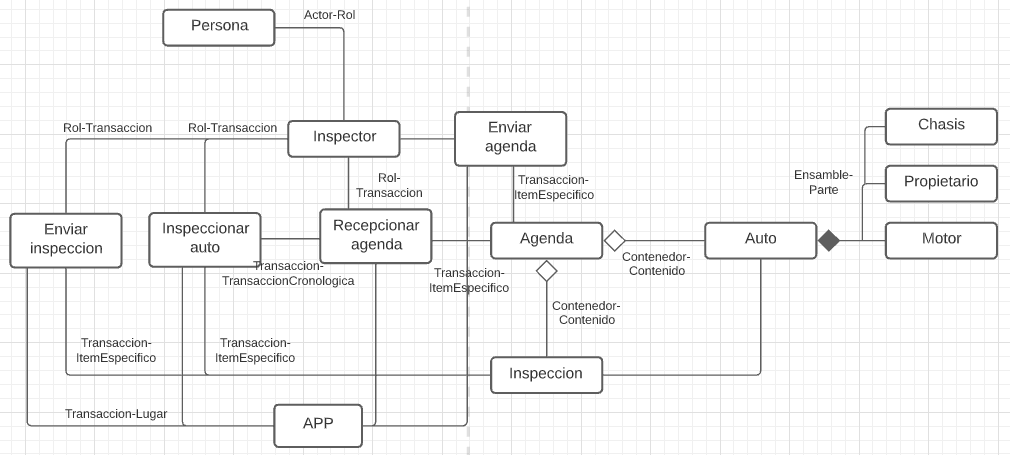
\includegraphics[width=\textwidth]{img/EjercicioInspectores.PNG}
\end{figure}

\begin{itemize}
\item Seguir los pasos para resolver el ejercicio. Empezar con Actor-Rol y seguir a partir de ahi.
\item No pensar en la implementación.
\item Se esta narrando como el inspector lleva adelante su trabajo.
\item No tiene sentido una Transacción sin un Item.
\item Nos interesan cuestiones del negocio en la resolución del ejercicio. \textit{Que se pueda cancelar algo ahora no es relevante.}
\item Inspección-Auto tiene una relación directa.
\end{itemize}

\subsection*{Ejemplo Sandwich}

\begin{figure}[!htb]
    \centering
    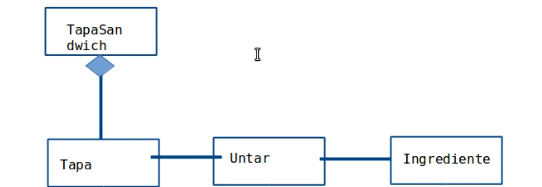
\includegraphics[width=0.6\textwidth]{img/ModeloSandwich.PNG}
\end{figure}

El siguiente ejemplo de código esta mal, no representa correctamente el modelo que se planteo para el sándwich.
\begin{minted}
[
frame=leftline,
framesep=5mm,
baselinestretch=1.2,
]
{java}
Sandwich s = new Sandwich();
Tapa t1 = new Tapa()
Tapa t2 = new Tapa()
Ingrediente i = new Ingrediente()

t1.set(i)
s.set(t1)
s.set(t2)
...
\end{minted}

Este en cambio, respeta el modelo planteado.
\begin{minted}
[
frame=leftline,
framesep=5mm,
baselinestretch=1.2,
]
{java}
Tapa t1 = new Tapa()
Tapa t2 = new Tapa()
Ingrediente i = new Ingrediente()
i.untar(t1)
Sandwich s = t2.montar(t1)
...
\end{minted}

\section*{Clase 3}
\section{Modelo relacional}
\begin{itemize}
\item Es un modelo a nivel lógico.
\item Va a intentar captar que es un conjunto, que es una relación formada por las tuplas.
\item Ahora la abstracción es un concepto matemático llamado relación. (de discreta)
\end{itemize}

\noindent\rule{\textwidth}{0.5pt}

\begin{itemize}
\item Dominio: Conjunto de valores homogéneos.
\item Producto cartesiano:  A x B, se define como el conjunto de pares (a,b) que cumplen que 'a' $\in$ A y 'b' $\in$ B
\end{itemize}

\noindent\rule{\textwidth}{0.5pt}

La cantidad de elementos que tiene es la cardinalidad de A por la de B. Llevándolo a código, al seleccionar Ciudades y Países en una consulta de SQL, se esta haciendo un producto cartesiano en el fondo, ya que se tienen todas las posibles combinaciones. Después se filtraran de acuerdo a la condición.

\begin{minted}
[
frame=leftline,
framesep=5mm,
baselinestretch=1.2,
]
{sql}
SELECT
FROM Ciudades, Paises
WHERE
\end{minted}

Una relación es un subconjunto de un producto cartesiano. Aquellos elementos del producto cartesiano tales que la ciudad pertenece al país.

En el modelo relacional, un \textbf{nombre de relación} R junto con una \textbf{lista de atributos }asociados se denomina\textbf{ esquema de relación }y se denota:

\begin{center}
 $R( A \_{1},A\_{2},..A\_{n})$
    
    \medskip
    
    Películas(nombre,año,director, oscars)
\end{center}

\medskip

\begin{itemize}
\item Con cada atributo tengo un dominio en particular asociado. \textit{Ej. nombre película en string, año en los naturales positivos} Películas esta en el subconjunto del producto cartesiano de todos los atributos.
\item Las\textbf{ instancias de la relación} son los elementos tengo cargados
\item Un elemento se llama una \textbf{tupla} si la tupla pertenece al subconjunto, es una instancia $t$ $\in$ Películas

\item El valor tomado por un atributo A en la tupla t se denota como t[A] o t.A
\textit{Por ejemplo}: t[director] = Quentin Tarantino (referencia al valor en la tupla $t$)

\item La cardinalidad en una relación R, es la cantidad de tuplas que posee.
\item Las relaciones las vemos como tabla, donde las columnas representan atributos y las filas representan tuplas. También se puede decir archivos, registros para filas, y campos para las columnas.
\end{itemize}


\subsection*{Restricciones}

\subsubsection*{De dominio}
\begin{itemize}
\item Las restricciones de dominio especifican que dado un atributo A de una relación R, el valor del atributo en una tupla $t$ debe pertenecer al dominio dom(A). Dominios posibles son naturales, reales, caracteres, string, bool, fechas, etc
\item Se puede permitir que los atributos tengan el valor nulo (NULL)
\item Deben ser atómicos (los atributos), no hay atributos compuestos (tarjeta de crédito) o multivaluados (conjunto de valores).
\item No pueden existir dos tuplas distintas que coincidan en los valores de todos sus atributos. Una tupla no puede estar dos veces.
\end{itemize}


\subsubsection*{Superclave}

\begin{itemize}
\item Generalmente existe un subconjunto SK del conjunto de atributos de R que cumple la condición de que dadas dos tuplas s, t $\in$ R, las mismas difieren en al menos uno de los atributos de SK. Si un subconjunto SK cumple esto, lo llamamos \textbf{superclave} de R.
\item Nos interesan las superclaves que son minimales (no admiten ningún subconjunto propio con la misma propiedad - no podemos achicar mas). Las llamamos \textbf{claves candidatas o claves}. Se elige una como \textbf{clave primaria}
\item Las claves primarias las subrayamos
\end{itemize}

\textit{Por ejemplo:}

\begin{center}
PRIMARY KEY (nombre\_pelicula, nombre\_director)
\end{center}

\medskip

No es minimal ya que podríamos tener\textit{ por ejemplo Quentin Tarantino, Tarantino}.


\subsubsection*{De integridad}
Un esquema de base de datos relacional S es un conjunto de esquemas de relación S junto con una serie de restricciones de integridad.

\begin{itemize}
\item \textbf{Restricciones de integridad de entidad:} la clave primaria de una relación no puede tomar el valor nulo. Quiere decir que tienen que ser identificables.
\item \textbf{Restricción de integridad referencial:} aquello a lo que referencia tiene que existir en la otra tupla de S referenciada. \textit{Cuando un conjunto de atributos FK de una relación R hace referencia a la clave primaria de otra relación S, entonces para toda tupla de R debe existir una tupla de S cuya clave primaria sea igual al valor de FK, a menos que todos los atributos de FK sean nulos.}
\end{itemize}

\medskip

\textit{Por ejemplo: Puedo tener una película sin actuación, pero no puedo tener una actuación sin película.}

\begin{itemize}
\item La clave foránea puede ser null.
\item Para agregar claves foraneas al crear una tabla: \textit{clave tipo REFERENCES tabla(atributo)}
\item Al intentar borrar de la tabla original, no te permite ya que esta referenciada desde la otra tabla.
\item Las claves foráneas las indicamos también con un subrayado punteado (de la cátedra)
\end{itemize}


\subsection*{Operaciones}

Las operaciones del modelo relacional se especifican a través de lenguajes como el álgebra relacional o el cálculo relacional. (Sección \ref{sec:relacional})
Podemos realizar consultas o actualizaciones (inserción, eliminación, modificación

\smallskip

\begin{itemize}
\item Las de consulta no violan ninguna restricción ya que no modifican ninguna relación.
\item Las de inserción de tuplas pueden violar restricciones de dominio, unicidad, de integridad de entidad o referencial.
\item Las de eliminación pueden violar la integridad referencial. Se puede rechazar la eliminación, eliminar en cascada, o poner NULL.
\item En las de modificación:
    \begin{itemize}
        \item Si se modifica una clave foránea, se debe verificar que sus nuevos valores referencien a una tupla existente de la relación referenciada, o bien sean todos nulos. De lo contrario se debería rechazar la operación.
        \item Si se modifica una clave primaria, puede violarse cualquiera de las restricciones de integridad, y se combinan las situaciones indicadas para inserción y eliminación.
    \end{itemize}
\end{itemize}

Estas restricciones llevan a lo que se conoce como \textbf{transacciones}. Son un conjunto de operaciones que quiero que el gestor me asegure que o bien se ejecuten, o no se hace nada. Si una transacción no puede terminar de realizarse porque una de sus operaciones viola alguna restricción de integridad, entonces debe dejarse la base de datos en el estado anterior al inicio de la misma.



\subsection*{Ejemplos}
\begin{itemize}
\item Los atributos multivaluados los tengo que poner en una tabla distinta. (Puedo tener varios teléfonos, los pongo en una tabla distinta)
\item En un atributo compuesto tengo que poner todos los atributos
\item ejemplo gerente-departamento, clave candidata, no puede haber dos filas con el nombre del gerente, se le agrega la palabra UNIQUE
\item ejemplo docentes relación ternaria
\end{itemize}



\section*{Clase 4}
\section{Practica: Modelo relacional}
\textit{Vamos a ver como mapear de un modelo de conceptual de Chen al relacional.
Obtener criterios para decidir cual es conveniente entre dos o mas modelos posibles.}

\begin{itemize}
\item Las entidades fuertes del conceptual pasan a ser entidades del relacional. 
\item La primary key pasa al relacional subrayada también,
\item Las relaciones binarias pasan también, tiene ambas ids como clave. Se subrayan cortado como foreign key (además del normal)
\item Si una interrelación tiene un atributo, va adentro de la relación.
\item La relación es un concepto matemático, la interrelación no (es mas conceptual).
\end{itemize}


\textbf{Entidades} A(\underline{idA},...) B(\underline{idB},...)

\medskip

\textbf{Relación} R(\underline{\underline{i}d\underline{A}},\underline{\underline{i}d\underline{B}})

\medskip

\begin{itemize}
\item En las relaciones unarios, para el id de la otra entidad (mismo tipo) se le pone otro nombre cambiado arbitrariamente.
\item En el caso binario 1:N (donde el valor mínimo de una es 0), como primary key de la relación usamos el id de la relación que tiene (1,1). Si ponemos a los dos, no seria mínima (seria una super clave). Hay que analizar también si conviene mover el atributo de la relación en la que tiene (1,1).
\end{itemize}

\medskip

\textbf{Entidades}
A(\underline{idA},...)
B(\underline{idB},...)

\medskip

\textbf{Relación}
R(\underline{i}d\underline{A},\underline{\underline{i}d\underline{B}})

\medskip

\textbf{Pasa a estar como}
B(\underline{idB},...,\underline{i}d\underline{A})


\begin{itemize}
\item Esto es para minimizar la cantidad de tablas.
\item Si tenemos el caso binario 1:N con opción de ninguno, la relación es necesaria, no se puede mover a una entidad. No esta bien ingresar algún carácter que indique que significa ninguno.
\end{itemize}

\medskip

\textbf{En el caso 1:1 hay varias opciones.}

\begin{itemize}
\item No olvidarse de definir las claves candidatas dependiendo el caso.
\item En las entidades débiles se tiene como PK el atributo discriminante y la clave de la entidad fuerte también (se marca como clave foránea además)
\end{itemize}

\medskip

\textbf{Relaciones ternarias}

\begin{itemize}
\item En el caso de las relaciones ternarias N:N:N se ponen como clave las tres ids, y las tres son foreign key.
\item En el caso 1:N:N se pone la relación con clave primaria de N y N, y la de 1 la tiene como foránea solo:
\end{itemize}
R(\underline{i}d\underline{A},\underline{\underline{i}d\underline{B}},\underline{\underline{i}d\underline{C}})

\medskip

\begin{itemize}
\item En 1:1:N las relaciones tenemos:
\end{itemize}
R(\underline{i}d\underline{A},\underline{\underline{i}d\underline{B}},\underline{\underline{i}d\underline{C}}) o 
R(\underline{\underline{i}d\underline{A}},\underline{i}d\underline{B},\underline{\underline{i}d\underline{C}})

\medskip

\begin{itemize}
\item No podemos ahorrarnos la tabla ya que estaríamos forzando a que todos los elementos tengan una asociación
\end{itemize}

\begin{itemize}
\item En 1:1:1 las claves candidatas son:
\end{itemize}
R(\underline{i}d\underline{A},\underline{\underline{i}d\underline{B}},\underline{\underline{i}d\underline{C}}) o 
R(\underline{\underline{i}d\underline{A}},\underline{i}d\underline{B},\underline{\underline{i}d\underline{C}}) o
R(\underline{\underline{i}d\underline{A}},\underline{\underline{i}d\underline{B}},\underline{i}d\underline{C})

\medskip

\begin{itemize}
\item Todas son claves candidatas (las 3), la PK es solo una. Las claves candidatas son igual de importantes, quiero que todas se verifiquen. Elijo una como PK, pero las otras siguen estando (UNIQUE).
\item En las especializaciones/generalizaciones (\textbf{caso disjunto y total (sin solapamiento)} - es uno o el otro), B es un A, y C es un A.
\item Tenemos las tres entidades, B y C con sus atributos propios y no comunes.
\item Los atributos comunes van en la tabla A. 
\item En A se puede agregar un atributo \emph{tipo} para decir en que tabla voy a poder buscar el resto de la información. (como es total, esto se puede asegurar que el tipo no sea nulo)
\end{itemize}


\subsection*{Taller}

\begin{itemize}
\item Si es una restricción de PK se le agrega el prefijo 'pk\_' Se hace también para las foreign keys (fn\_). 
\item Conviene definirlas como constraint, ya que es mas robusto que definirla en la creación inicial porque ante un error nos indica mas claramente el problema.
\end{itemize}

\medskip

Ejemplo de agregado de una clave como CONSTRAINT (parte 2 y 4):
\begin{minted}
[
frame=leftline,
framesep=5mm,
baselinestretch=1.2,
]
{sql}
ALTER TABLE paradas ADD CONSTRAINT pk_paradas PRIMARY KEY(cod_parada);

ALTER TABLE colectivos_por_parada ADD CONSTRAINT fk_colectivos_por_parada
FOREIGN KEY(cod_parada) REFERENCES paradas(cod_parada);
\end{minted}

\medskip

Intente provocar una violación a la restricción de integridad de entidad de
la tabla colectivos por parada a través de un INSERT.
\begin{minted}
[
frame=leftline,
framesep=5mm,
baselinestretch=1.2,
]
{sql}
INSERT INTO colectivos_por_parada VALUES(NULL,44)
\end{minted}

\medskip

Intente provocar una
violación a la restricción de integridad referencial definida, a través de un INSERT en la
tabla que considere apropiada.
\begin{minted}
[
frame=leftline,
framesep=5mm,
baselinestretch=1.2,
]
{sql}
INSERT INTO colectivos_por_parada VALUES(99999999,44);
\end{minted}

\medskip

Intente provocar una violación a la restricción de integridad referencial definida, a través de un DELETE en la tabla
que considere apropiada
\begin{minted}
[
frame=leftline,
framesep=5mm,
baselinestretch=1.2,
]
{sql}
DELETE FROM paradas WHERE cod_parada=1000086;
\end{minted}

\medskip

Intente modificar el código de la parada 1004561 por el código 1007800
utilizando un script de UPDATE. ¿Es posible hacerlo? No, es referida por la tabla colectivos\_por\_parada todavia.
\begin{minted}
[
frame=leftline,
framesep=5mm,
baselinestretch=1.2,
]
{sql}
UPDATE paradas SET cod_parada=1007800 WHERE cod_parada=1004561;
\end{minted}

\medskip

Formas de delete (aplican tambien al ON UPDATE):
\begin{itemize}
\item ON DELETE NO ACTION: Si hay referencias a otra tabla, no la borra.
\item ON DELETE CASCADE: Elimina las referencias también (las tuplas) en forma de cascada sucesivamente
\item Esta también SET NULL (cuidado si tenemos NOT NULL, sigue valiendo) y SET DEFAULT
\end{itemize}

\smallskip

Las autoridades de la Dirección de Transito quieren que sea
posible cambiar el código de una parada, modificando automáticamente todas las filas que
hacen referencia a ella en otras tablas. Modifique para ello el script de CREATE TABLE,
definiendo una CONSTRAINT de ON UPDATE en la tabla correspondiente.
\begin{minted}
[
frame=leftline,
framesep=5mm,
baselinestretch=1.2,
]
{sql}
ALTER TABLE colectivos_por_parada ADD CONSTRAINT fk_colectivos_por_parada 
FOREIGN KEY(cod_parada) REFERENCES paradas(cod_parada)
ON UPDATE CASCADE;
\end{minted}

Es posible actualizar la tabla ahora.


\newpage


\section*{Clase 5}
En realidad se dio durante la tercera clase debido a que caía un feriado en el día de la clase. (A partir de este punto no es del todo correcto el orden de clases mencionado en este apunte)
\section{UML}
Mas información para cada uno de estos diagramas en el apunte de Análisis de la Información. Acá solo se dejan breves descripciones.
\subsection*{Diagramas de actividad}
Para representar dinámicas del negocio, donde el tiempo va transcurriendo de arriba hacia abajo. Nos dan pie a los casos de uso.

\subsection*{Diagrama de Casos de uso}
Cada una de las actividades esta representada acá. Puede ocurrir que después algún caso de uso se parta en varios mas, que se representarían en otro diagrama. 

\subsection*{Diagrama de estados}
Se realizan para algunos de los objetos creados para indicar el paso de estados. No se indica que hace que pase de estados, sino los cambios posibles.

\subsection*{Diagrama de paquetes}
\begin{itemize}
\item Los negocios por lo general tienen múltiples contextos, que analizados con las herramientas empiezan a tomar forma en paquetes (parte de nuestros negocios). 
\item Permiten concentrar la dinámica de nuestro negocio desde el punto de vista del negocio.
\item Paquetes de un alto nivel, paquetes de nivel intermedio, y después de mas bajo nivel.
\item Los paquetes se asocian con componentes, que a su vez estan asociados a nodos.
\item Son muy intuitivos, pero poco rigurosos. Hay que tener en cuenta la inversión en la cadena de dependencia (principio). Esto no es tenido en cuenta en los siguientes gráficos de paquetes.
\end{itemize}


\begin{figure}[!htb]
    \centering
    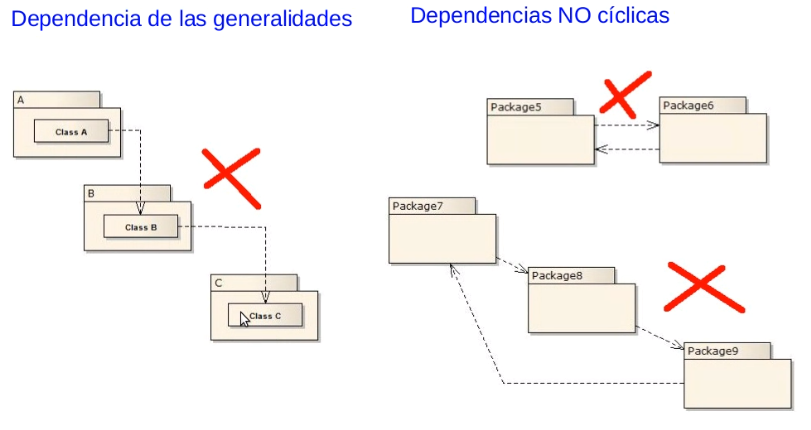
\includegraphics[width=0.6\textwidth]{img/paq.PNG}
\end{figure}

Para que nuestro diseño goce de esto, el nivel superior debe estar compuesto por abstracciones/generalidades, y los niveles inferiores de cuestiones concretas que dependen de las generalidades. 

\begin{figure}[!htb]
    \centering
    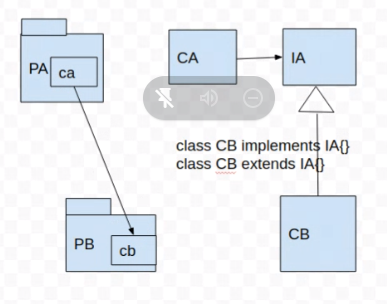
\includegraphics[width=0.8\textwidth]{img/paqbien.PNG}
\end{figure}

% imagen
% ca y ia dentro del paquete PA
Se cumple la inversión en la cadena de dependencia
Hay que hacer el gráfico de la derecha para cuestiones vinculadas al diseño. % cuestion para ser mas cuidadoso en uml

\subsection*{Otras cuestiones de UML mencionadas}
\begin{itemize}
\item Composición, no puede existir la clase A sin la clase B, seria incompatible. Corresponde a un Ensamble-Parte.
\item Agregación, puedo construir tipo A sin B. Se agrega un agregador de B. Cuando lo tenga, A no es dueño de B.\textit{ (Llevándolo a C++, A no seria el encargado de destruir a B, ya que no es dueño de B)}
\item De uso, asociación, solamente utiliza al objeto.
\end{itemize}



\section*{Clase 6}
\section{Git}
Se deja un resumen de lo que se dijo (estos temas ya se vieron en otras materias principalmente). Si se quiere ver sobre el funcionamiento interno de Git  revisar las notas en el apunte de Sistemas Operativos.

\begin{itemize}
\item Estados del sistema para conservar para el futuro
\item Compartirlo para el resto del equipo
\item Cada commit tiene archivos, fecha, mensaje, commits ancestros.
\item El único requisito es que la historia no tenga ciclos.
\item El equipo debe decidir como organizarse.
\item Combinar ideas base y flujos pre-armados.
\item Issues para ir relacionando la información que tenemos.
\item Commits atómicos
\item Una sola razon para todo lo que cambio.
\item No depende de cambios externos.
\item Historia lineal para proyectos simples, costoso para separar lineas de trabajo 
\item El control de versiones es naturalmente distribuido.
\item Branches para proyectos mas grandes donde hay mas gente.
\item Cuidado con los conflictos en los merge.
\item Cuidado con los Shutgun Surgery si se esta resolviendo en distintas ramas.
\item Hay una correlación entre mal diseño y no saber lo que hace el software.
\item Pull requests para revisar la calidad del codigo y aplicacion. Tienen que ser atomicos tambien (una sola razon para lo que cambio). Similar a como queremos en los commits.
\item Integracion continua para compilar y testear de forma automatica. Con esto integrar el trabajo realizado. (artefactos son archivos que quiero que se guarden)
\item Despliegue continuo para probarlo en diferentes entornos.
\item Cuidado con mantener dos branches largos. (van divergiendo cada vez mas)
\item Branches de entorno
\item Git Flow, la idea es tener dos branches a largo plazo. Master y Develop. Desde Develop salen Feature Branches que mergeamos devuelta a Develop. Git Flow agrega Release Branches (las creamos a partir de Develop, y solo le agregamos bug fixes), una vez que es adecuado para entregar al cliente, se hace el merge a master. Estan las branches de Hotfixes para emergencias, se les hace merge a Master y a Develop.
\end{itemize}


%links a recursos

\section*{Clase 7}
\section{SQL}

\begin{itemize}
\item Es un lenguaje no procedural, basado en el calculo relacional de tuplas.
\item Tiene 9 partes el ISO SQL actualmente, las mas importantes son 2, la de Foundation (2) y Information and Definition Schemas (11). Se las conoce como Core SQL.
\item Es una gramática libre de contexto. Su sintaxis puede describirse a través de reglas de reglas de producción.
\item Para estudiar esto lo mejor es ir a la documentación, tiene las opciones y ejemplos.
\end{itemize}


\subsection*{Tipos de dato (en el estándar)}
\begin{itemize}
\item INTEGER
\item SMALLINT
\item FLAOT
\item DOUBLE PRESICION
\item NUMERIC(i,j): tipo numérico exacto. Permite especificar la precisión i y la escala j en dígitos.
\item CHARACTER(n) longitud fija
\item CHARACTER VARYING(n) longitud variable VARCHAR(n)
\item DATE: yyyy-mm-dd
\item TIME(i)
\item TIMESTAMP(i)
\item BOOLEAN: true, false, unknown - Logica de tres valores.
\item CLOB: Character Large Object - Generalmente guardados aparte 
\item BLOB: Binary Large Object
\end{itemize}


El usuario puede definir tipos de dato también:
\begin{itemize}
\item CREATE DOMAIN CODIGO\_PAIS AS CHAR(2)
\end{itemize}


\subsubsection*{Configuraciones}
\begin{itemize}
\item Las columnas pueden configurarse con valores por defecto con DEFAULT o auto incrementales AUTO\_INCREMENT.
\item PRIMARY KEY
\item UNIQUE: una columna o conjunto de columnas no puede estar con valores repetidos.
\item En el modelo relacional una relación es un conjunto cuyos elementos son las tuplas. Por lo tanto, una tupla no puede estar repetida en una relación. 
\item En SQL esto no pasa, pueden repetirse. Se conoce como multiset o bag of tuples.
\end{itemize}

\subsection*{Consultas}

\begin{itemize}
\item La consulta básica es SELECT ... FROM ... [ WHERE ... ]
\item SELECT es equivalente a la proyección del álgebra relacional, y el WHERE a la selección del álgebra relacional. La diferencia es que el WHERE no elimina duplicados, no es estrictamente una proyección.
\end{itemize}


\medskip

\subsubsection*{Condiciones en el WHERE}
\begin{itemize}
\item Podemos comparar atributos con otros, o con valores.
\item Realizar un pattern matching
\item Que este o no en un conjunto
\item Que este en rangos
\item Que no sea nulo
\item Que exista
\item Que este o no en una tabla
\item Permite poner otra consulta adentro también, podemos generar anidamientos de consultas.
\end{itemize}


\medskip
\textit{Nota: el distinto se escribe con <> , y no se pone =NULL se pone es IS NULL}

\subsubsection*{Otros}
\medskip
\begin{itemize}
\item Podemos usar alias para el FROM (tambien para el SELECT para redenominar atributos) con AS para las tablas.
\item Se permiten operaciones adentro del SELECT (+,-,*,/, etc)
\item Tenemos funciones de agregación: SUM, COUNT, AVG, MAX, MIN
\item DISTINCT después del SELECT elimina duplicados
\item Para comparar patrones LIKE
\end{itemize}


\subsubsection*{Join}
\begin{itemize}
\item Clausula JOIN para evitar escribir todas las condiciones de junta. INNER JOIN ... ON, NATURAL JOIN, LEFT/RIGHT/FULL OUTER.
\item Si no escribo OUTER, sql interpreta que queremos INNER.
\item Se puede plantear con el WHERE tambien.
\end{itemize}



\subsubsection*{Operaciones de conjuntos}
\begin{itemize}
\item UNION, INTERSECT, EXCEPT, deben de tener compatibilidad de tipos (misma cantidad de columnas). Si no se agrega ALL se eliminan duplicados
\end{itemize}


\subsubsection*{Ordenamiento y paginación}
\begin{itemize}
\item ORDER BY por defecto es ascendente
\item La forma estándar de la paginación es OFFSET n ROWS FETCH FIRST .. ROWS ONLY. Algunos SGBD implementan LIMIT o TOP
\end{itemize}

\subsubsection*{Agrupamiento}

\begin{itemize}
\item Queremos hacer un resumen de ciertos datos.
\item La agregación colapsa las tuplas que coinciden con una serie de atributos.
\item Formato: \mint{sql}|SELECT ... FROM ... GROUP BY ... [HAVING ...]|
\item Puedo usar sin agregar los atributos por los que agrupo. El resto si los quiero los tengo que agregar. (Promedio, suma, cantidad, etc) (Resumir muchos valores en uno)
\item HAVING es para filtrar con algún valor en particular, es una clausula opcional.
\item Si en una agregación no se especifican atributos de agregación, el resultado tendrá una única tupla.
\end{itemize}


\subsection*{Subconsultas}

\begin{figure}[!htb]
    \centering
    \includegraphics[width=0.8\textwidth]{img/subconsultas.PNG}
\end{figure}

\begin{itemize}
\item Dependencia con lo de afuera
\item Si no depende se dice que no están correlacionadas, tiene menor costo.
\item Me doy cuenta si esta correlacionada si usamos algo de la consulta mayor en la subconsulta. Puede pasar que en la ejecución el gestor la logre separar.
\end{itemize}


\subsubsection*{Tablas intermedias}
Para poder usar el resultado de consultas intermedias, definimos esas tablas como sigue:
\mint{sql}|WITH nombre AS consulta|

\medskip
Esta tambien el WITH RECURSIVE que amplia el poder expresivo de SQL.

\begin{itemize}
\item No se guardan en ningún lado, son solo sintaxis. Seria lo mismo que poner la consulta adentro de la otra.
\item Son mucho mas claras para documentar la consulta.
\end{itemize}

\subsection*{Inserciones}

Es posible agregar valores a las tablar mediante:
\mint{sql}|INSERT INTO tabla VALUES (valores)|

\medskip
Se puede insertar también el resultado de un SELECT, los tipos tienen que ser compatibles

\medskip
En cualquiera de los siguientes casos no se inserta el valor.
\begin{itemize}
\item Se asigna a una columna un valor fuera de su dominio
\item Se omitió una columna que no podía ser NULL
\item Se puso en NULL una columna que no podía ser NULL
\item La clave primaria asignada ya existe en la tabla
\item Una clave foránea hace referencia a una clave no existente
\end{itemize}


\subsection*{Eliminaciones}

\mint{sql}|DELETE FROM ... FROM ...WHERE ...|

Si se tenia ON DELETE RESTRICT no se elimina la fila.

\subsection*{Modificaciones}
\mint{sql}|UPDATE ... SET ... WHERE ...|

Para cada fila t que cumpla alguna condición de las siguientes no se actualiza.
\begin{itemize}
\item Se modifica una columna asignándole un valor fuera de su dominio
\item Se pasó a NULL una columna que no podía tomar ese valor
\item Se asignó a la clave primaria un valor que ya existe en la tabla
\item Se modificó una clave foránea para hacer referencia a una clave no existente
\item Se configuro ON UPDATE RESTRICT
\end{itemize}


\subsection*{Eliminando tablas}

Para tablas: DROP TABLE tabla [RESTRICT|CASCADE]

\medskip
Para esquemas: DROP SCHEMA esquema [RESTRICT|CASCADE]


\subsection*{Otras funciones}
\begin{itemize}
    \item SUBSTRING(string FROM start FOR length)
    \item UPPER/LOWER(string)
    \item CHAR\_LENGTH(string)
    \item CAST( attr AS tipo)
    \item EXTRACT(campo FROM attr) - (para las fechas)
    \item || para concatenar
\end{itemize}

\begin{minted}
[
frame=leftline,
framesep=5mm,
baselinestretch=1.2,
]
{sql} 
SELECT nro_factura ,
    CAST(
        CAST(año_venc AS CHAR) || '-' ||
        SUBSTRING(('0' || CAST(mes_venc AS VARCHAR)
                FROM (2 CAST(mes_venc <10 AS INTEGER)) FOR 2)
        || '-' ||
        SUBSTRING(('0' || CAST(dia_venc AS VARCHAR))
                FROM (2 CAST(dia_venc <10 AS INTEGER)) FOR 2) AS DATE
        ) AS fecha_venc
FROM Facturas f;
\end{minted}

\subsection*{Estructura CASE}
\mint{sql}|CASE WHEN .. THEN .. ELSE ..END|
Permite agregar lógica de programación a la salida de una sentencia de sql.


\subsection*{Vistas en SQL}
Podemos mostrar a los usuarios determinadas partes de la base de datos a través de las vistas. Se puede decir que es una tabla virtual, el resultado de una operación ejecutada en ese momento. 

Se crean de la siguiente forma:
\begin{minted}
[
frame=leftline,
framesep=5mm,
baselinestretch=1.2,
]
{sql}
CREATE VIEW nombreVista
[(nuevoNombreColumna [,...])] AS consulta
[WITH [CASCADED | LOCAL] CHECK OPTION]
\end{minted}


Ejemplo

\begin{minted}
[
frame=leftline,
framesep=5mm,
baselinestretch=1.2,
]
{sql}
CREATE VIEW EMP_ACC AS
SELECT Nombre, Documento, Sector, Sucursal FROM EMPLEADOS;
\end{minted}


El usuario vería solo la información provista por:

\begin{minted}
[
frame=leftline,
framesep=5mm,
baselinestretch=1.2,
]
{sql}
SELECT * FROM EMP_ACC;
\end{minted}


En las vistas también se pueden buscar casos específicos, agrupar, combinar, son condiciones que se agregan en el SELECT.

Se pueden eliminar vistas con 

\begin{minted}
[
frame=leftline,
framesep=5mm,
baselinestretch=1.2,
]
{sql}
DROP VIEW nombreVista [RESTRICT | CASCADE]
\end{minted}


RESTRICT si tengo algún objeto relacionado, no ejecuta el borrado
CASCADE borra todos los objetos dependientes relacionados, aquellos que hagan referencia a la vista

\subsubsection*{Cambios en las vistas}

Como los cambios en las tablas bases se ven automáticamente en las vistas, también se pueden modificar datos a través de las vistas y que modifique las tablas base. Para que pueda pasar esto, no debe de tener operadores conjuntistas, el operador DISTINCT, funciones agregadas, o GROUP BY

Para ser actualizable, FROM debe referenciar a solo una tabla base.

\subsubsection*{Materialización}

Las vistas pueden tomar mucho tiempo si son complejas, se puede evitar con la materialización. Esto realiza una tabla temporal que almacena la vista. Se mantiene la vista por cada cambio de los datos.

\subsubsection*{¿Para que usarlas?}

Las vistas se usarían para:
\begin{itemize}
\item Ocultar información
\item Administración simple de permisos
\item Personalizar datos
\item Menor complejidad
\item Proporcionar compatibilidad con las consultas ya armadas
\item Integridad de los datos
\item Combinar datos de servidores
\end{itemize}


\subsubsection*{Privilegios sobre ellas}

Se otorgan privilegios a los usuarios de la siguiente forma
\begin{minted}
[
frame=leftline,
framesep=5mm,
baselinestretch=1.2,
]
{sql}
GRANT {Lista Privilegios | ALL PRIVILEGES}
ON NombreObjeto
TO {ListaIdentifiadoresAutorizacion | PUBLIC}
[WITH GRANT OPTION]
\end{minted}

Se pueden revocar con: \mint{sql}|REVOKE|


\newpage

\section*{Clase 8}
\section{Practica: Taller SQL}
\begin{itemize}
    \item Es un lenguaje declarativo, le digo que quiero y de alguna forma lo hace.
    \item ¿Cual forma de hacer algo es mas performante? No es fácil saberlo, generalmente el motor se puede dar cuenta cual hacer.
    \item Las cadenas de caracteres con comillas simples. Las comillas dobles las interpreta como que queremos acceder a una columna.
    \item Operadores lógicos AND, OR, NOT
    \item Evitar usar SELECT * ... , ya que no queda definida la consulta en ese momento.
    \item Definir forma de almacenar datos, esto es buena practica, pero trae problemas ante alguna equivocación.
    \item Con los operadores de conjuntos por defecto no hay duplicados.
    \item No usar NATURAL JOIN en aplicativos para evitar problemas a futuro, ya que la consulta no queda totalmente definida. Si el esquema de la tabla cambia, nos enteramos cuando se ejecuta.
    \item El resultado de una consulta se puede usar como tabla en la entrada de otra consulta (subconsulta)
    \item Cuando agrupo puedo devolver alguna de las columnas agrupadas, o resultados que surgen de alguna función de agregación.
\end{itemize}

\subsection*{1 - Devuelva todos los datos de las notas que no sean de la materia 75.1}

\begin{itemize}
\item Con que difiera alguno de ellos ya nos alcanza. Fijarse con De Morgan. Plantearlo con \mint{sql}|AND| es un error común, ya que obligamos a que sea distinto si o si, en este caso hay que negar el resultado si queremos el \mint{sql}|AND|.
\end{itemize}


\begin{minted}
[
frame=leftline,
framesep=5mm,
baselinestretch=1.2,
]
{sql} 
SELECT * FROM notas WHERE codigo <> 75 OR numero <> 1
\end{minted}

\subsection*{2 Devuelva para cada materia dos columnas: una llamada “código” que contenga una concatenación del código de departamento, un punto y el numero de materia, con el formato “XX.YY” (ambos valores con dos dígitos, agregando ceros a la izquierda en caso de ser necesario) y otra con el nombre de la materia.}

\begin{minted}
[
frame=leftline,
framesep=5mm,
baselinestretch=1.2,
]
{sql} 
SELECT to_char(codigo,'fm00') || '.' || to_char(numero,'fm00') AS "codigo",nombre
FROM materias
\end{minted}

\begin{itemize}
\item Con el doble pipe lo estamos concatenando con un punto en el medio.
\item Con el AS renombramos la columna inicial.
\item Documentación del \href{https://www.postgresql.org/docs/current/functions-formatting.html}{to\_char}.
\end{itemize}



\subsection*{3 - Para cada nota registrada, devuelva el padrón, código de departamento, número de materia, fecha y nota expresada como un valor entre 1 y 100.}

\begin{minted}
[
frame=leftline,
framesep=5mm,
baselinestretch=1.2,
]
{sql} 
SELECT padron,codigo,numero,fecha,nota*10 AS "nota"
FROM notas
\end{minted}

\subsection*{4 -  Ídem al anterior pero mostrando los resultados paginados en páginas de 5 resultados cada una, devolviendo la segunda página}

\begin{minted}
[
frame=leftline,
framesep=5mm,
baselinestretch=1.2,
]
{sql} 
SELECT padron,codigo,numero,fecha,nota*10 AS "nota"
FROM notas
OFFSET 5 ROWS FETCH FIRST 5 ROWS ONLY
\end{minted}


\begin{itemize}
\item Esta \mint{sql}|LIMIT 5| después del offset también.
\item Si no le digo algún orden, no se que me va a devolver. Si queremos garantizarnos los resultados, hay que tomarse la costumbre de ordenar de la forma que no deje ambigüedad en las filas. En este caso agregando antes del \mint{sql}|FETCH| un \mint{sql}|ORDER BY padron| - Así evitamos tener un orden indeterminado.
\end{itemize}

\begin{minted}
[
frame=leftline,
framesep=5mm,
baselinestretch=1.2,
]
{sql} 
SELECT padron,codigo,numero,fecha,nota*10 AS "nota"
FROM notas
ORDER BY padron,codigo,numero,fecha
OFFSET 5 ROWS FETCH FIRST 5 ROWS ONLY;
\end{minted}

\subsection*{5 - Ejecute una consulta SQL que devuelva el padrón y nombre de los alumnos cuyo apellido es “Molina”}
\begin{minted}
[
frame=leftline,
framesep=5mm,
baselinestretch=1.2,
]
{sql} 
SELECT padron,nombre
FROM alumnos
WHERE apellido = 'Molina';
\end{minted}

\begin{itemize}
\item No es lo mismo que: (el siguiente estaría mal)
\end{itemize}

\begin{minted}
[
frame=leftline,
framesep=5mm,
baselinestretch=1.2,
]
{sql} 
SELECT padron,nombre
FROM alumnos
WHERE apellido = 'molina';
\end{minted}


\begin{itemize}
\item Postgres es una base de datos CASE SENSITIVE. Por lo que no devolvería nada en este caso. \mint{sql}|LIKE| es case sensitive también, se puede usar \mint{sql}|ILIKE| (no es estándar y no aprovecha índices)
\end{itemize}

\begin{minted}
[
frame=leftline,
framesep=5mm,
baselinestretch=1.2,
]
{sql} 
SELECT padron,nombre
FROM alumnos
WHERE apellido ILIKE 'Molina';
\end{minted}


\begin{itemize}
\item Otra alternativa es llevándolo a una forma común con Upper o Lower.
\end{itemize}

\begin{minted}
[
frame=leftline,
framesep=5mm,
baselinestretch=1.2,
]
{sql} 
SELECT padron,nombre
FROM alumnos
WHERE Upper(apellido) = 'MOLINA';
\end{minted}


\subsection*{6 - Obtener el padrón de los alumnos que ingresaron a la facultad en el año 2010}

\begin{minted}
[
frame=leftline,
framesep=5mm,
baselinestretch=1.2,
]
{sql} 
SELECT padron
FROM alumnos
WHERE fecha_ingreso>='2010-01-01' AND fecha_ingreso<='2010-12-31';
\end{minted}

Con otra sintaxis:
\begin{minted}
[
frame=leftline,
framesep=5mm,
baselinestretch=1.2,
]
{sql} 
SELECT padron
FROM alumnos
WHERE fecha_ingreso BETWEEN '2010-01-01' AND '2010-12-31';
\end{minted}

\subsection*{7 - Obtener la mejor nota registrada en la materia 75.15}

\begin{minted}
[
frame=leftline,
framesep=5mm,
baselinestretch=1.2,
]
{sql} 
SELECT MAX(nota)
FROM notas
WHERE codigo=75 AND numero=15;
\end{minted}

\subsection*{8 - Obtener el promedio de notas de las materias del departamento de código 75}

\begin{minted}
[
frame=leftline,
framesep=5mm,
baselinestretch=1.2,
]
{sql} 
SELECT AVG(nota)
FROM notas
WHERE codigo=75;
\end{minted}


\subsection*{9 - Obtener el promedio de nota de aprobación de las materias del departamento de código 75.}

\begin{minted}
[
frame=leftline,
framesep=5mm,
baselinestretch=1.2,
]
{sql} 
SELECT AVG(nota)
FROM notas
WHERE codigo=75 and nota>=4;
\end{minted}

\subsection*{10 - Obtener la cantidad de alumnos que tienen al menos una nota}

\begin{minted}
[
frame=leftline,
framesep=5mm,
baselinestretch=1.2,
]
{sql} 
SELECT COUNT(DISTINCT padron)
FROM notas
\end{minted}


\begin{itemize}
\item \mint{sql}|COUNT| solo cuenta los distintos de nulos, si queremos que sean distintas lo hacemos con \mint{sql}|DISTINCT|.
\end{itemize}


\subsection*{11 - Devolver los padrones de los alumnos que no registran nota en materias}


\begin{itemize}
\item Estamos realizando la operación de conjuntos: A - B
\end{itemize}

\begin{minted}
[
frame=leftline,
framesep=5mm,
baselinestretch=1.2,
]
{sql} 
(SELECT padron
FROM alumnos)
EXCEPT
(SELECT padron
FROM notas)
\end{minted}

\begin{minted}
[
frame=leftline,
framesep=5mm,
baselinestretch=1.2,
]
{sql} 
SELECT padron
FROM alumnos
WHERE padron
NOT IN
(SELECT DISTINC(padron) FROM notas)
\end{minted}

\subsection*{12 - Con el objetivo de traducir a otro idioma los nombres de materias y departamentos, devolver en una única consulta los nombres de todas las materias y de todos los departamentos}

\begin{minted}
[
frame=leftline,
framesep=5mm,
baselinestretch=1.2,
]
{sql} 
(SELECT nombre
FROM materias)
UNION
(SELECT nombre
FROM departamentos)
\end{minted}

\subsection*{13 - Devolver para cada materia su nombre y el nombre del departamento}


\begin{itemize}
\item Con \mint{sql}|JOIN|
\end{itemize}
\begin{minted}
[
frame=leftline,
framesep=5mm,
baselinestretch=1.2,
]
{sql} 
SELECT m.nombre, d.nombre
FROM materias AS m, departamentos AS d
WHERE m.codigo=d.codigo 
\end{minted}


\begin{itemize}
\item Otras forma para hacerlo:
\end{itemize}
\begin{minted}
[
frame=leftline,
framesep=5mm,
baselinestretch=1.2,
]
{sql} 
SELECT m.nombre, d.nombre
FROM materias AS m INNER JOIN  departamentos AS d
ON m.codigo=d.codigo 
\end{minted}

\begin{minted}
[
frame=leftline,
framesep=5mm,
baselinestretch=1.2,
]
{sql} 
SELECT m.nombre, d.nombre
FROM materias AS m INNER JOIN departamentos AS d
USING (codigo) 
\end{minted}


\subsection*{14 - Para cada 10 registrado, devuelva el padrón y nombre del alumno y el nombre de la materia correspondientes a dicha nota}

\begin{minted}
[
frame=leftline,
framesep=5mm,
baselinestretch=1.2,
]
{sql} 
SELECT a.padron,a.nombre,m.nombre
FROM alumnos AS a, notas AS n, materias AS m
WHERE n.nota=10 AND a.padron=n.padron
AND n.codigo=m.codigo AND n.numero=m.numero;
\end{minted}

\begin{minted}
[
frame=leftline,
framesep=5mm,
baselinestretch=1.2,
]
{sql} 
SELECT a.padron,a.nombre,m.nombre
FROM notas AS n
INNER JOIN materias AS m ON m.numero=n.numero AND m.codigo=m.codigo
INNER JOIN alumnos AS a ON a.padron=n.padron
WHERE n.nota=10;
\end{minted}

\begin{minted}
[
frame=leftline,
framesep=5mm,
baselinestretch=1.2,
]
{sql} 
SELECT n.padron,a.nombre AS nombre_alumno,m.nombre AS nombre_materia
FROM (notas n INNER JOIN alumnos a USING (padron)) INNER JOIN materias m 
USING (codigo,numero)
WHERE n.nota = 10
\end{minted}

\subsection*{15 - Listar para cada carrera su nombre y el padrón de los alumnos que estén anotados en ella. Incluir también las carreras sin alumnos inscriptos}

\begin{minted}
[
frame=leftline,
framesep=5mm,
baselinestretch=1.2,
]
{sql} 
SELECT c.nombre,i.padron
FROM carreras AS c LEFT OUTER JOIN inscripto_en AS i
USING (codigo)
\end{minted}

\begin{minted}
[
frame=leftline,
framesep=5mm,
baselinestretch=1.2,
]
{sql} 
SELECT carreras.nombre,alumnos.nombre,alumnos.apellido
FROM carreras
LEFT OUTER JOIN inscripto_en ON inscripto_en.codigo = carreras.codigo
LEFT OUTER JOIN alumnos ON inscripto_en.padron = alumnos.padron
\end{minted}

\subsection*{16 - Ídem punto anterior pero teniendo en cuenta únicamente alumnos con padrón mayor a 75000}

% REVISAR
\begin{minted}
[
frame=leftline,
framesep=5mm,
baselinestretch=1.2,
]
{sql} 
SELECT carreras.nombre,alumnos.nombre,alumnos.apellido
FROM carreras
LEFT OUTER JOIN inscripto_en ON inscripto_en.codigo = carreras.codigo
LEFT OUTER JOIN alumnos ON inscripto_en.padron = alumnos.padron
WHERE alumnos.padron > 75000
\end{minted}

\begin{minted}
[
frame=leftline,
framesep=5mm,
baselinestretch=1.2,
]
{sql} 
SELECT c.nombre,i.padron
FROM carreras AS c LEFT OUTER JOIN inscripto_en AS i
USING (codigo)
WHERE padron > 75000
\end{minted}

\begin{minted}
[
frame=leftline,
framesep=5mm,
baselinestretch=1.2,
]
{sql} 
SELECT c.nombre, ie.padron
FROM taller_4.CARRERAS c 
LEFT OUTER JOIN taller_4.inscripto_en ie ON (ie.codigo = c.codigo AND ie.padron > 75000);
\end{minted}

\subsection*{17 - Listar el padrón de aquellos alumnos que tengan m´as de una nota en la materia 75.15}


\begin{itemize}
\item De esta forma no se tiene la mejor performance, ya que se esta revisando fila por fila con el valor de la consulta mayor.
\end{itemize}

\begin{minted}
[
frame=leftline,
framesep=5mm,
baselinestretch=1.2,
]
{sql} 
SELECT a.padron
FROM alumnos as a
WHERE 
(SELECT count(n.nota)>1 FROM notas AS n
WHERE n.padron=a.padron AND n.codigo=75 AND n.numero=15)
\end{minted}

\begin{itemize}
\item Otra opción poniendo el >1 afuera de la subconsulta.
\end{itemize}
\begin{minted}
[
frame=leftline,
framesep=5mm,
baselinestretch=1.2,
]
{sql} 
SELECT a.padron
FROM alumnos as a
WHERE 
(SELECT count(n.nota) FROM notas AS n
WHERE n.padron=a.padron AND n.codigo=75 AND n.numero=15) >1 
\end{minted}

\begin{minted}
[
frame=leftline,
framesep=5mm,
baselinestretch=1.2,
]
{sql} 
SELECT DISTINCT n1.padron
FROM notas n1, notas n2
WHERE n1.codigo = 75 AND n2.codigo = 75
AND n1.numero = 15 AND n2.numero = 15
AND n1.padron = n2.padron
AND n1.fecha <> n2.fecha
\end{minted}

\subsection*{18 - Obtenga el padrón y nombre de los alumnos que aprobaron la materia 71.14 y no aprobaron la materia 75.15}

\begin{minted}
[
frame=leftline,
framesep=5mm,
baselinestretch=1.2,
]
{sql} 
SELECT A.PADRON, A.NOMBRE 
FROM ALUMNOS A
WHERE EXISTS(SELECT 1 FROM NOTAS N WHERE N.NOTA >= 4
            AND N.CODIGO = 71 AND N.NUMERO = 14 
            AND N.PADRON = A.PADRON) 
AND NOT EXISTS(SELECT 1 FROM NOTAS N WHERE N.NOTA >= 4 
            AND N.CODIGO = 71 AND N.NUMERO = 15 
            AND N.PADRON = A.PADRON);
\end{minted}
\begin{itemize}
\item Se fija que exista un aprobado en la materia, y que no exista un aprobado en la otra.
\end{itemize}


Otra forma:
\begin{minted}
[
frame=leftline,
framesep=5mm,
baselinestretch=1.2,
]
{sql} 
SELECT A.PADRON, A.NOMBRE 
FROM ALUMNOS A
WHERE A.PADRON IN (SELECT N.PADRON FROM NOTAS N WHERE N.NOTA >= 4 
			 AND N.CODIGO = 71 AND N.NUMERO = 14 ) 
AND A.PADRON NOT IN (SELECT N.PADRON FROM NOTAS N 
				WHERE N.NOTA >= 4 
				AND N.CODIGO = 71 AND N.NUMERO = 15 );
\end{minted}

\subsection*{19 - Obtener, sin repeticiones, todos los pares de padrones de alumnos tales que ambos alumnos rindieron la misma materia el mismo día. Devuelva también la fecha y el código y numero de la materia}

\begin{minted}
[
frame=leftline,
framesep=5mm,
baselinestretch=1.2,
]
{sql} 
SELECT DISTINCT N.PADRON PADRON, NOTA.PADRON PADRON2,
N.FECHA, N.CODIGO, N.NUMERO FROM TALLER_4.NOTAS N
INNER JOIN
TALLER_4.NOTAS AS NOTA
ON NOTA.PADRON < N.PADRON
AND NOTA.FECHA = N.FECHA 
AND N.CODIGO = NOTA.CODIGO 
AND N.NUMERO = NOTA.NUMERO;
\end{minted}


\subsection*{20 - Para cada departamento, devuelva su código, nombre, la cantidad de materias que tiene y la cantidad total de notas registradas en materias del departamento. Ordene por la cantidad de materias descendente}

\begin{minted}
[
frame=leftline,
framesep=5mm,
baselinestretch=1.2,
]
{sql} 
SELECT d.codigo, d.nombre, COUNT(DISTINCT n.numero) AS "cant_mat",
COUNT(*) AS "cant_not"
FROM notas n INNER JOIN materias m USING (codigo, numero) 
INNER JOIN departamentos d USING (codigo)
GROUP BY d.codigo, d.nombre
ORDER BY COUNT(DISTINCT n.numero) DESC
\end{minted}

\begin{minted}
[
frame=leftline,
framesep=5mm,
baselinestretch=1.2,
]
{sql} 
WITH cant AS (
	SELECT codigo, COUNT(numero) AS cant FROM materias GROUP BY codigo
), notasD AS (
	SELECT codigo, COUNT(notas) AS cant FROM notas GROUP BY codigo
)
SELECT d.codigo,d.nombre, c.cant, n.cant
FROM departamentos d, cant c, notasD n
WHERE d.codigo = c.codigo AND d.codigo=n.codigo
ORDER BY c.cant DESC

\end{minted}

\subsection*{21 - Para cada carrera devuelva su nombre y la cantidad de alumnos inscriptos. Incluya las carreras sin alumnos}

\begin{minted}
[
frame=leftline,
framesep=5mm,
baselinestretch=1.2,
]
{sql} 
SELECT c.nombre, COUNT(i.padron)
FROM carreras c LEFT OUTER JOIN  inscripto_en i USING (codigo)
GROUP BY c.codigo, c.nombre
\end{minted}

Es importante contar un atributo que no tenga nulos, así lo cuentan.

\subsection*{22 - Para cada alumno con al menos tres notas, devuelva su padrón, nombre, promedio de notas y mejor nota registrada}

\begin{minted}
[
frame=leftline,
framesep=5mm,
baselinestretch=1.2,
]
{sql} 
SELECT a.padron, a.nombre, AVG(n.nota) AS promedio, MAX(n.nota) AS mejor_nota
FROM alumnos AS a, notas AS n
WHERE a.padron = n.padron
GROUP BY a.padron, a.nombre
HAVING COUNT(*) >= 3
\end{minted}

\begin{itemize}
\item Condiciones que se aplican grupo a grupo no van en el WHERE, ya que viene en una etapa después.
\item Puedo evaluar cosas que después no devuelvo en el HAVING.
\end{itemize}


\subsection*{23 - Obtener el código y numero de la o las materias con mayor cantidad de notas registradas.}

\begin{minted}
[
frame=leftline,
framesep=5mm,
baselinestretch=1.2,
]
{sql} 
SELECT n.codigo, n.numero, COUNT(*)
FROM notas n
GROUP BY n.codigo, n.numero
HAVING COUNT(*) >= ALL (
    SELECT COUNT(*)
    FROM notas n
    GROUP BY n.codigo, n.numero
)
\end{minted}

\begin{minted}
[
frame=leftline,
framesep=5mm,
baselinestretch=1.2,
]
{sql} 
WITH cantidades AS (SELECT n.codigo, n.numero, COUNT(*) AS cant
	FROM notas n
	GROUP BY n.codigo, n.numero)
SELECT codigo, numero, cant
FROM cantidades c
WHERE c.cant = (SELECT MAX(cant) FROM cantidades)
\end{minted}


\begin{itemize}
\item No es valido ordenarlo y devolver el primero, puede darse el caso de que varios coincidan con el mejor valor. Queremos todas con la mayor cantidad.
\item No esta permitido realizar un MAX del COUNT en el HAVING.
\item No podemos anidar funciones de agregación.
\end{itemize}

\subsection*{24 - Obtener el padrón de los alumnos que tienen nota en todas las materias}

\begin{minted}
[
frame=leftline,
framesep=5mm,
baselinestretch=1.2,
]
{sql} 

SELECT padron
FROM alumnos a
WHERE NOT EXISTS (
    SELECT * 
    FROM materias m 
    WHERE NOT EXISTS (
        SELECT * 
        FROM notas n
        WHERE n.padron = a.padron
		      AND n.codigo = m.codigo
		      AND n.numero = m.numero
        )
)

\end{minted}

\begin{itemize}
\item Es una división.
\item Buscamos los alumnos con nota en todas las materias, tal que para los alumnos no exista materia en la que no tiene nota.
\item Alumnos para los que no existe una materia en la que no existe una nota de ese alumno en esa materia
\end{itemize}



\begin{minted}
[
frame=leftline,
framesep=5mm,
baselinestretch=1.2,
]
{sql} 

SELECT padron
FROM alumnos a
WHERE NOT EXISTS (
    (SELECT codigo, numero FROM materias)
    EXCEPT
    (SELECT codigo, numero FROM notas n WHERE n.padron=a.padron)
)

\end{minted}


\begin{itemize}
\item Primer conjunto: todas las materias
\item Segundo conjunto: todas las materias en las que un alumno tiene nota
\end{itemize}


\begin{minted}
[
frame=leftline,
framesep=5mm,
baselinestretch=1.2,
]
{sql} 


SELECT padron
FROM notas n
GROUP BY n.padron
HAVING COUNT( DISTINCT(to_char(codigo,'fm00') ||'.'|| to_char(numero,'fm00') ))
       =
       (SELECT COUNT(*) FROM materias)

\end{minted}


\begin{itemize}
\item Contar cuantas materias hay y cuento en cuantas materias tiene nota. Tiene que dar lo mismo
\item El DISTINCT solo recibe un atributo, no es estandar que tome dos.
\end{itemize}

\subsection*{25 - Obtener el promedio general de notas por alumno (cuantas notas tiene en promedio un alumno), considerando únicamente alumnos con al menos una nota}

\begin{minted}
[
frame=leftline,
framesep=5mm,
baselinestretch=1.2,
]
{sql} 


SELECT CAST(COUNT(*) AS DECIMAL) / COUNT(DISTINCT padron)
FROM notas n;

\end{minted}

Cuidado con realizar la división entera, esta trunca el resultado.
\newpage

\section*{Clase 9}
\section{Principios de diseño}
Los principios de diseño (SOLID), la ley de Demeter, separación de incumbencias están siempre presentes en cada decisión que tomemos sobre la arquitectura.

Los criterios generales son:
\begin{itemize}
\item Economía
\item Visibilidad
\item 'Espaciamiento'
\item Simetría
\item Emergencias
\end{itemize}


\subsection*{Economía}
\begin{itemize}
\item Tiene que ver con el listado de métodos que componen una misma interfaz.
\item Busca evitar complejidades innecesarias, flexibilidad innecesaria, y enfocarnos en la usabilidad mas que en la reusabilidad.
\item La interfaz tiene que estar limpia y económica. Tener la mínima cantidad de métodos necesarios que sean útiles.
\end{itemize}


\subsection*{Visibilidad}

\begin{itemize}
\item La especificación en términos de interfaces y herencia o implementación suele ser obscura, poco visible y difícil de entender y navegar.
\item Es preferible la composición y delegación que la herencia.
\end{itemize}


\begin{figure}[!htb]
    \centering
    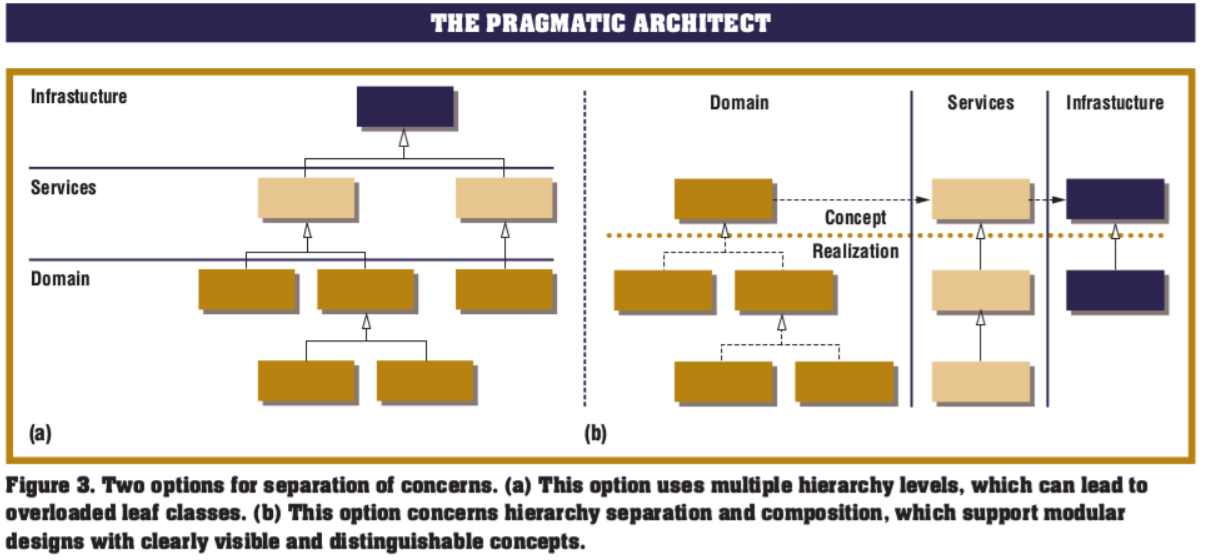
\includegraphics[width=0.8\textwidth]{img/VisibilidadPatrones.PNG}
\end{figure}

\subsection*{'Espaciamiento'}
\begin{itemize}
\item Tiene que ver con el desacoplamiento.
\item Contribuye a la visibilidad y el reuso.
\item Busca definir cuales son los roles de cada componente del diseño, lo cual nos ayuda a separarlos. Si nos cuesta definirlos es que esta en demasiadas cosas.
\item Distancia entre responsabilidades funcionales claramente distintas y autónomas conduce a componentes.
\item  Espaciado entre las perspectivas de uso de un componente conduce a interfaces con rol específico.
\item La separación entre grupos de componentes conduce a capas y subsistemas.
\item El espacio entre el contrato y la realización conduce a interfaces explícitas e implementaciones separadas.
\end{itemize}



\subsection*{Simetría}

\begin{itemize}
\item Facilita la comprensión, comunicación, extensión y mantenimiento.
\end{itemize}

\begin{figure}[!htb]
    \centering
    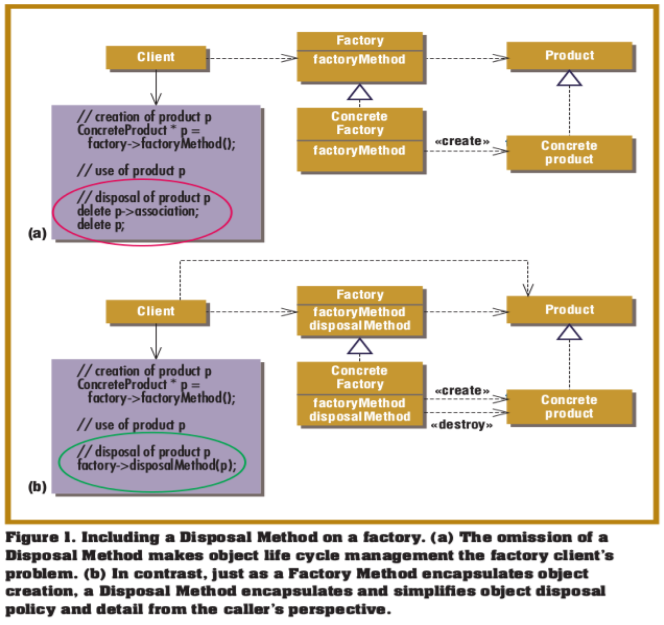
\includegraphics[width=0.8\textwidth]{img/simetriaPatrones.PNG}
    \caption{Diagrama de arriba se instancian instancias a través de un Factory que no destruye los objetos. Esto es asimétrico, solo crea no destruye.}
\end{figure}



\subsection*{Emergencias}
\begin{itemize}
\item Tiene que ver con algo que emerge por su forma, por su repetición en contexto similar.
\item Facilita la organización y escalabilidad.
\item Emergente es el comportamiento de auto-organización y junto con el control son a menudo la clave para la escalabilidad, eficiencia y economía en las arquitecturas
\end{itemize}


\section{Patrones}

\begin{itemize}
\item Situaciones que se empiezan a repetir y se puede solucionar de la misma forma.
\item Los definimos por un contexto en la cual se plantea un problema, el problema (\textit{que según Bushman puede estar compuesto por fuerzas que se contraponen y los patrones buscan balancear}), y por la solución (relación/interacción entre varias clases)
\item Nadie inventa patrones, estos se descubren.
\item Esta implícito en el nombre del patrón todo lo que constituye.
\item Son buena documentación de diseño.
\end{itemize}

\textit{Más adelante se sigue con patrones de diseño.}

\textit{Parte de donde surge la idea (arquitectura - de los edificios): A Pattern Language - Christopher Alexander }


\section{Patrones de arquitectura}
Para saber cuando usar cada uno, necesitamos saber el contexto y el problema que se presenta. Orientados a organizar la plataforma en la cual se va a construir el sistema.

\subsection*{Layer}

\begin{itemize}
\item Idea: Tenemos un sistema que tiene un volumen grande, en el cual aparecen conceptos de distinto nivel de abstracción.
\item Hay diferentes capas con distintos niveles de abstracción. \textit{Ej. Teléfonos presentado en clase, comunicación, tarifas de las llamadas, las impresoras, administración del locutorio} Cuando tenemos esto conviene el uso de este patrón.
\item Cada capa (layer) utiliza un servicio de la capa superior. Permite reutilizar partes.
\item Las ventajas son reuso, cambiabilidad, desarrollo simultaneo, ya que las capas se pueden manejar por separado.
\item La desventaja es un diseño mas elaborado
\item El patrón no ofrece una respuesta a cuantas capas tengo que tener, esto depende de los requerimientos. \textit{Ej. Modelo OSI de redes}
\end{itemize}

\begin{figure}[!htb]
    \centering
    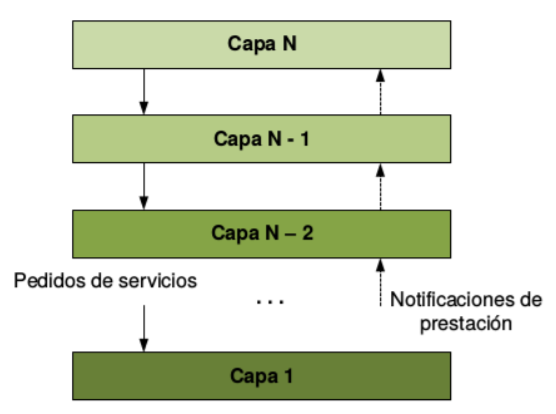
\includegraphics[width=0.8\textwidth]{img/LayerPatron.PNG}
\end{figure}

\subsection*{EA}
\begin{itemize}
\item Enterprise Architecture
\item Es un Mega patrón, compuesto por muchos patrones. (se va a ver mejor mas adelante)
\item Es conveniente usarlo cuando hay un sistema cliente-servidor (remoto). También cuando hay usuarios concurrentes, múltiples interfaces de usuario, reglas de negocio y datos persistentes.
\item Se usa desacoplando los diferentes 'tiers' para lograr separar incumbencias.
\item Las ventajas son el reuso y la cambiabilidad,
\item La desventaja es un mayor trabajo.
\end{itemize}


\begin{figure}[!htb]
    \centering
    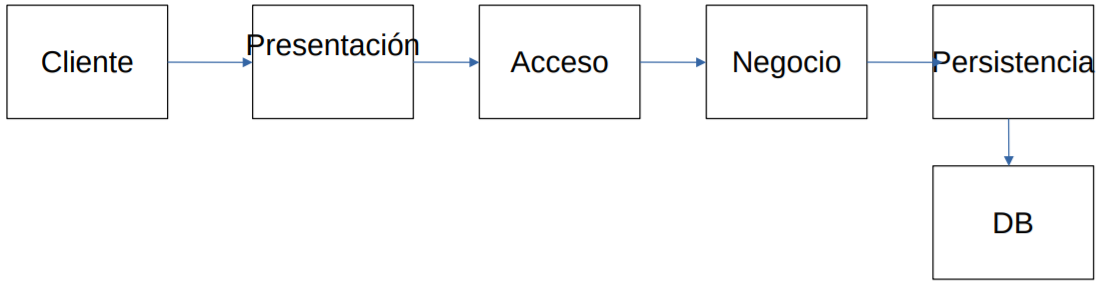
\includegraphics[width=0.8\textwidth]{img/EAPatron.PNG}
    \caption{Ejemplo}
\end{figure}


\subsection*{Microkernel}
El patrón arquitectónico de Microkernel se aplica a un sistema de software que debe ser capaz de adaptarse a los cambios en los requisitos del sistema. Separa un núcleo funcional mínimo de la funcionalidad extendida y de las piezas específicas del cliente. El microkernel también sirve como enchufe para conectar estas extensiones y coordinar su colaboración
\begin{itemize}
\item Conviene utilizarlo en sistemas de larga vida que deben evolucionar ante cambios de distinto tipo con diferente frecuencia.
\item Con un sistema monolítico se complica.
\item Asigna componentes esenciales al microkernel y distribuye las componentes entre los servers.
\item Esta compuesto por External Servers, el Microkernel, y el Internal Server
\item Las ventajas son que soporta cambios con menor impacto.
\item La desventaja es un diseño mas elaborado
\end{itemize}

\begin{figure}[!htb]
    \centering
    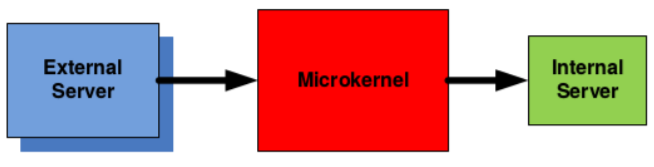
\includegraphics[width=0.8\textwidth]{img/MicrokernelPatron.PNG}
\end{figure}


\subsection*{Pipe Filter}

\begin{itemize}
\item Conviene usarlo cuando debemos procesar un stream de datos, y este procesamiento se puede descomponer en N procesamientos atómicos.
\item Permite sistemas mas reutilizables, es reuso.
\item Para usarlo, distribuir los procesamientos en filtros, definir el formato de datos en los pipes y definir la implementación.
\item La ventaja es el reuso y el rápido prototipado.
\item La desventaja es que no se puede usar en sistemas críticos ya que no podemos controlar el estado global. (en caso de que falle un filtro)
\end{itemize}

\begin{figure}[!htb]
    \centering
    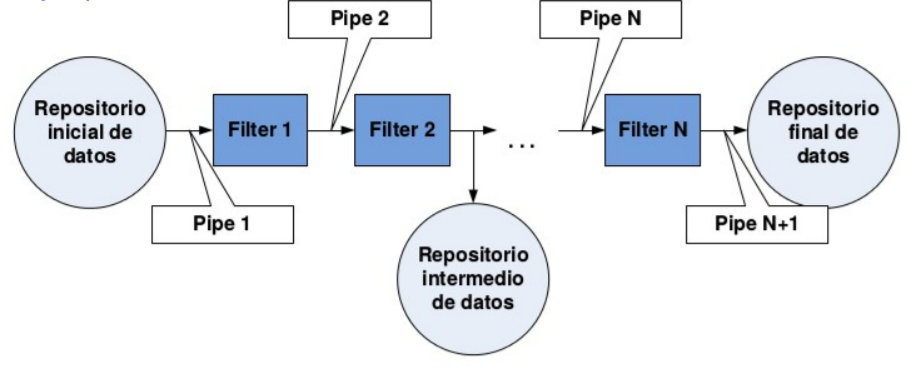
\includegraphics[width=0.8\textwidth]{img/PipeFilterPatron.PNG}
\end{figure}


\subsection*{MVC}

\begin{itemize}
\item Modelo-Vista-Controlador
\item Es conveniente usarlo cuando es necesario contar con interfaces de usuario múltiples y diferentes para los mismos datos, flexibles y cambiables.
\item El usuario solo interactúa con el modelo a través de los controladores.
\item El modelo esta desacoplado, se vuelve transportable.
\item Los ve en las vistas.
\item Viene de la mano con el patrón Observer, se encarga de propagar los cambios en el modelo.
\item La ventaja es la reusabilidad y facilidad de cambios y extensión
\item Las desventajas son que se tiene un mayor diseño y que hay que tener cuidado con las bibliotecas que ya implementan algo.
\end{itemize}

\begin{figure}[!htb]
    \centering
    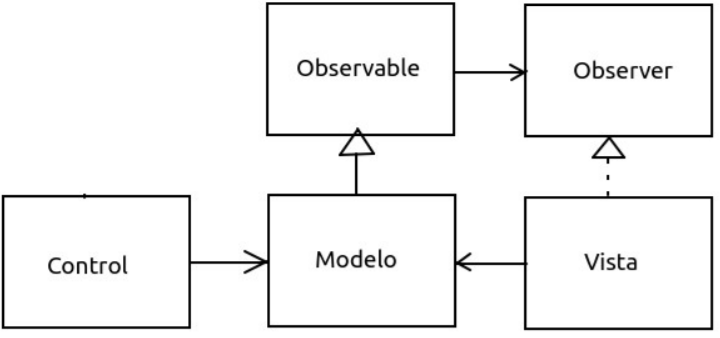
\includegraphics[width=0.7\textwidth]{img/MVCPatron.PNG}
\end{figure}

\subsection*{Broker}
El Broker es un patrón de arquitectura que se utiliza para estructurar sistemas de software distribuidos con componentes desacoplados que interactúan por invocaciones de servicios remotos. Esto quiere decir que, si un componente necesita un servicio de otro que está en otra ubicación que no conoce, el broker se encarga de proporcionar la conexión. Si los componentes manejaran la comunicación por sí mismos, el sistema se enfrentaría a diversas dependencias y limitaciones.
\begin{itemize}
\item Es necesario usarlo cuando se tiene que contar con procesamiento distribuido a partir de objetos distribuidos. También cuando es necesario abstraerse de la tecnología que implementa la comunicación entre procesos.
\item Conviene siempre que se pueda no distribuir los objetos.
\item Las ventajas son la cambiabilidad, la portabilidad, y el reuso.
\item Las desventajas son la baja eficiencia, dificultad de desarrollo y que no tolera fallas.
\item Esta compuesto por el Broker, dos proxies (Stub y Skeletor) que se ocupan de la serializacion e ida y vuelta.
\end{itemize}

\begin{figure}[!htb]
    \centering
    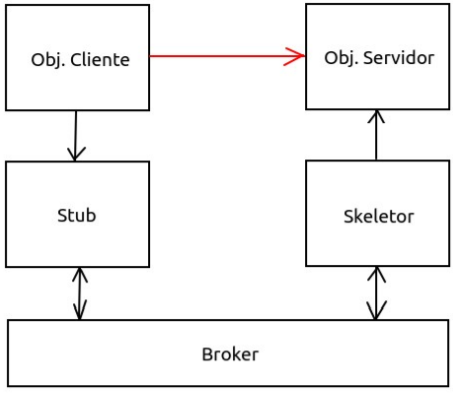
\includegraphics[width=0.5\textwidth]{img/BrokerPatron.PNG}
\end{figure}








\section*{Clase 10 y 12}
\section{Practica ejercicios}
\subsection*{Enunciado ejercicio}
Una empresa de desarrollos electrónicos planea lanzar al mercado el instrumento universal de diagnóstico 
que ha bautizado con el nombre de “RobotDoc”. Para este proyecto nos ha contratado el desarrollo del 
software y nos ha pedido una primera impresión. 

\medskip
El aparato será una especie de robot ambulante y tendrá como parte de su arquitectura una computadora 
donde se ejecutará el software, una carcaza que le dará usabilidad desde el punto de vista ergonométrico y un
componente electrónico que permite conectarse con otros instrumentos que no poseen medios de 
comunicación estándard como las computadoras (RJ45, USB, etc.). Está orientado a centros de salud que no 
poseen un sistema integrado de información.

\medskip
Se pensó a “RobotDoc” como un recolector de información de los diferentes consultorios/laboratorios donde 
se realizan los siguientes estudios: electroencefalograma, electrocardiograma, resonancia magnética, rayos X
y electromiograma. En estos casos el aparato se conecta con otros instrumentos y consume datos tales como 
señales muestreadas. En el caso de los laboratorios se conecta con las computadoras y consume datos de 
informes.

\medskip
El operador se desplaza a cada lugar y al tomar los datos ingresa información del paciente de manera que al 
final del recorrido por diferentes áreas del hospital queda agrupada la información por paciente. Es decir que 
para cada paciente habrá un conjunto de estudios con los cuales los diferentes médicos que lo atiendan 
podrán elaborar un diagnóstico utilizándola. 

\medskip
“RobotDoc” es compartido por varios médicos, los cuales acceden a él y elaboran su diagnóstico con el 
enfoque de su especialidad. Para este fin “RobotDoc” debe presentar la funcionalidad de “diagnosticar” con 
enfoques preestablecidos para cada especialidad (gastroenterología, cardíaco, clínico, neurológico, etc.). Los 
diagnósticos no podrán ser realizados si no fue recolectada la información de todos los estudios solicitados. 
Aquellos estudios que daten de más de 15 días deberán repetirse, es decir que quedan invalidados para ser 
utilizados en la elaboración de un diagnóstico, solo serán usados como informativos. Cada paciente tendrá 
una historia clínica conformada por todos los estudios realizados y los diagnósticos realizados.
La información de los diferentes estudios deben poder relacionarse a partir de un conjunto determinado de 
algoritmos que aún no fueron entregados. Esta funcionalidad es una especie de asistencia al médico que 
permiten detectar diferentes fenómenos, medir distintas magnitudes, correlacionar sucesos de diferentes 
estudios, procesar señales e imágenes. 

\medskip
Los diagnósticos incluirán posibles causas, explicaciones, recomendaciones y prescripciones realizadas por 
el médico especialista en base a la información recolectada y procesada. Los profesionales para utilizarlos 
deben registrarse previamente y serán agrupados por el administrador según su especialidad. Las secretarias 
de las áreas del hospital podrán acceder a los estudios e imprimirlos para ser entregados a los pacientes. 
Todos los usuarios deben estar agrupados a efectos de poder acceder al uso.

\medskip
Se cree que la experiencia compartida por profesionales de la salud con diferentes visiones y sugerencias 
respecto de las interfaces de usuario así como la aparición de nuevos instrumentos a conectar generará al año
de uso la producción de un segundo release del software que nos encargan.

\medskip
Toda la información de “RobotDoc” se almacena en un servidor del hospital, aunque este es el límite de 
nuestro contrato, es decir no incluye el desarrollo de ninguna parte de este servidor.

\medskip
Hemos decidido elaborar, para presentar a la empresa, un Modelo de Dominio que muestre el 
funcionamiento de este negocio para validarlo y una definición preliminar de la Arquitectura donde se 
justifique cada una de las partes incluidas. 

\medskip
Un año después … hay que agregar la funcionalidad de realizar diagnósticos con enfoque de medicina del 
deporte para lo cual es necesario conectarse con un aparato de electrocardiogramas de esfuerzo diferente a 
todos los manejados hasta ahora. También incluiremos los cambios sugeridos a algunas de las interfaces de 
los diagnósticos por imágenes. Por favor indique en que lugar de la arquitectura definida anteriormente 
impactarán estos tres cambios.

\subsection*{Modelo de dominio}

\begin{figure}[!htb]
    \centering
    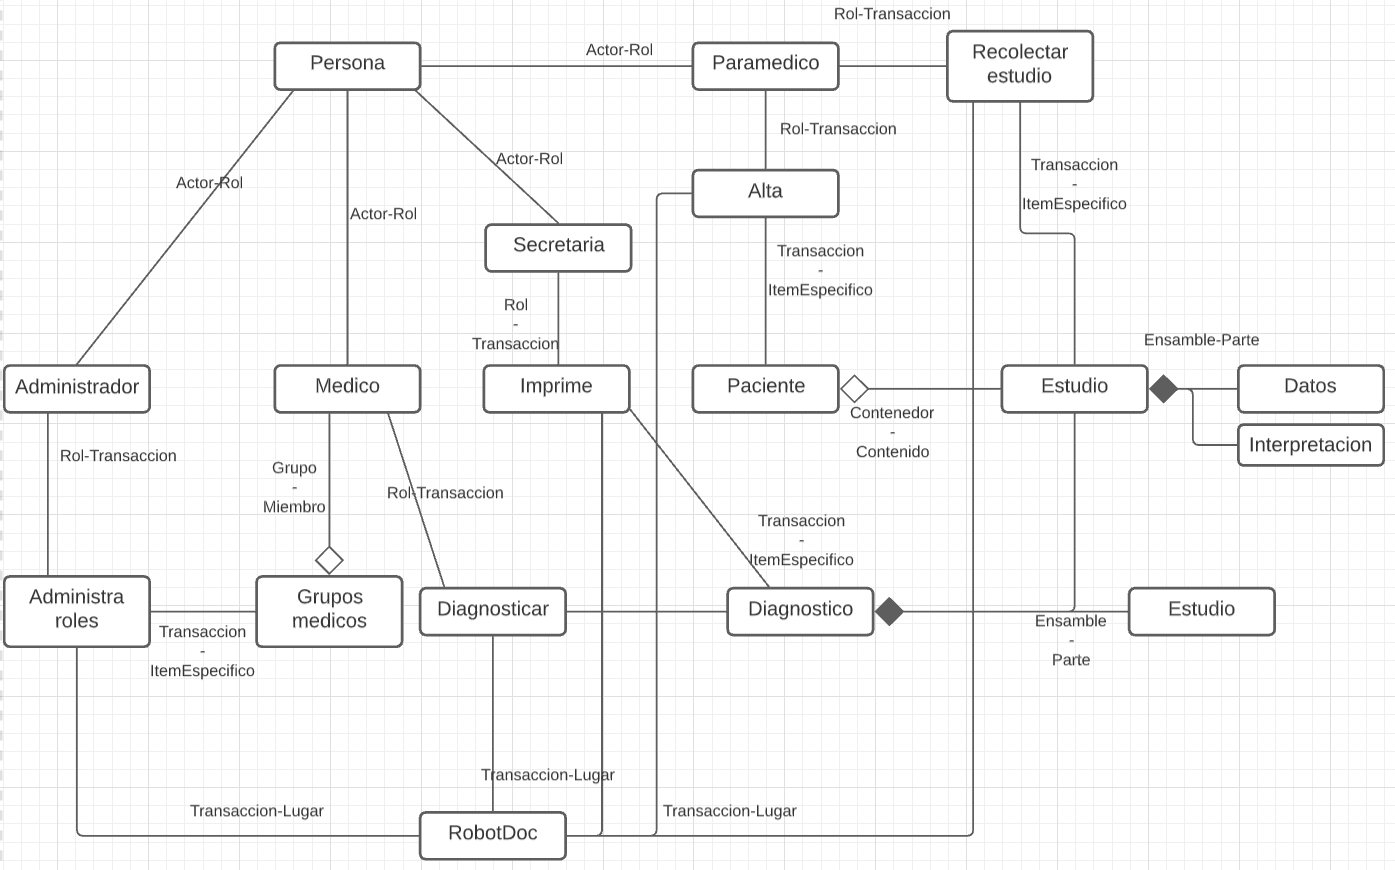
\includegraphics[width=\textwidth]{img/EjercicioRobotDoc.PNG}
\end{figure}


\begin{itemize}
\item Para ir armándolo siempre seguir los pasos.
\item El rol tiene que ver con la interacción con el sistema.
\item Se puede agregar también grupos de secretarias, y relacionar con secretaria
\end{itemize}

\subsection*{Arquitectura}


\begin{itemize}
\item Tenemos distintos niveles de abstracción, usaríamos el patrón Layer para resolver esta cuestión. Permitiendo desacoplar los recursos al encapsular en cada una de las capas (el layer).
\item Cada external server (Diagnosticos) tiene un MVC
\item Mas alto nivel es diagnostico
\item El microkernel esta compuesto por 3 componentes que deben de tener su sentido. Se debe de tener mas de una dirección de cambio. En nuestro caso se quiere conectar a aparatos nuevos, y nos dice que se van a hacer estudios nuevos. Por lo que es probable que tengamos que agregar médicos con especialidades nuevas.
\end{itemize}

\begin{figure}[!htb]
    \centering
    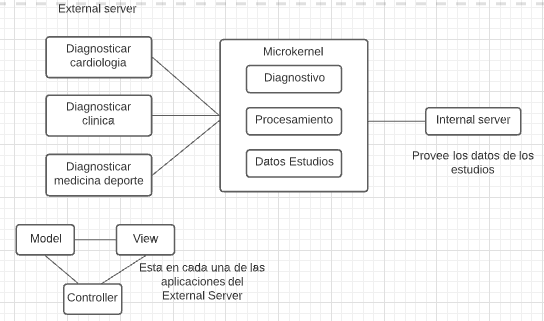
\includegraphics[width=0.8\textwidth]{img/EjercicioArquitectura.PNG}
\end{figure}

% hacer matriz
% no le pusimos reglas
% El hecho de que la arquitectura requiera flexibilidad va a tener impacto en las distintas vistas. (Esto ya lo implica la introducción del MVC)
% Hay un tema de seguridad tambien, y del manejo de señales

% (para ver como afectan las distintas vistas)

% administrador es probable que no vaya a cambiar las tareas
% operador e inspector pueden llegar a tener cambios
% ea, sistema cliente servidor que se tiene que conectar a la red con el sistema viejo
% microkernel con capas, layers, ordenadas segun el grado de abstraccion
% ea arriba quiere decir que lo reusable es el microkernel
% hay que tener en cuenta las cuestiones independientemente de la arquitectura

\textit{Se dio una clase antes en la que se explico el parcial y la parte de paradigmas. Uní lo de paradigmas con la siguiente clase por ser corto.}

\section{Paradigmas}
\begin{itemize}
\item En una manera es un modo de pensar. En nuestro caso es un enfoque, una forma de pensar un problema.
\item C, C++, Java, son lenguajes usados para modelar conceptos y relacionarlos con otros. No están pensados para procesar datos. (Las ultimas versiones están incluyendo ya cuestiones de programación funcional)
\item Programación lógica que esta orientado a la demostración de teoremas. Navega estructuras simbólicas complejas según un conjunto de reglas. (\textit{Ej. Prolog})
\item La programación funcional, algoritmos complejos resueltos a partir de la composición de funciones. Es ideal para implementar algoritmos y procesar datos.
\item La idea es resolver los distintos aspectos que nos presenta un problema con el enfoque adecuado.
\end{itemize}




\section{Programación Funcional}

\begin{itemize}
\item Es un paradigma de programación basado en funciones matemáticas y declarativo. La ejecución de programas es ir evaluando las funciones.
\item Algunos ejemplos de lenguajes son Lisp, Haskell, Erlang y esta en otros multiparadigma.
\item Es simulado al resolver problemas cuya solución natural es funcional (Git, Docket, REST, React)
\item \textit{Se ve el tema de forma más completa en Lenguajes Formales.}
\end{itemize}

\subsection*{Características}

\begin{itemize}
\item Las \textbf{funciones se tratan como cualquier otro valor}. 
\begin{itemize}
    \item Tienen expresiones literales
    \item Pueden ser argumentos a funciones
    \item Pueden ser retornadas por otras funciones
\end{itemize}
\item Las funciones tienen que ser \textbf{predecibles}, producir la misma salida para una determinada entrada. Esto se rompe con aleatoriedad, entrada/salida y estados variables (tiempo/ubicación)
\item Se tiene que tener \textbf{inmutabilidad} también. Evaluar una función no modifica el estado del programa. En lugar de actualizar valores, se crean nuevos valores. El estado mutable genera race conditiones, acciones a distancia, y cada mutación puede romper variantes. Las funciones no pueden cambiar su entrada o contexto.
\item En funcional se suele usar la \textbf{recursividad}. Se define una función en termino de si misma. Se determina un caso base y uno recursivo que nos acerca al final. Una propiedad que hay que aprovechar es la de llamados de cola. Remplaza el stack frame en lugar de crear uno nuevo. 
\item \textbf{Funciones de orden superior}, son funciones que operan sobre otras funciones como argumento. Abstraen estructuras de control, describen la intención con la que se manipulan valores. Algunos ejemplos son map (aplica una función a cada uno de los elementos), filter (devuelve los que cumplen la condición) y reduce (combina valores). Se prefiere el uso de funciones de orden superior a la recursividad.
\item El modelo de ejecución es la especificación del orden y ejecución del programa. El aplicativo evalúa cada argumento, remplaza los argumentos por su valores y evalúa el cuerpo hasta llegar a una expresión primitiva (los no funcionales usan solo esta forma). El otro orden es el normal. Busca el llamado a función mas externo y lo remplaza por su cuero sustituyendo los argumentos por su expresión. Puede evaluar fu unciones que son ciclos infinitos en orden aplicativo.
\item Hay que minimizar los efectos implícitos no locales.
\end{itemize}






\section*{Clase 11}

% justificar en 4 renglones o menos porque usamos x patron de arquitectura
% identificar cuales son los requerimientos no funcionales
% hacer la matriz donde aparecen las vistas y los requerimientos por el otro lado
% marcar en cada celda el impacto que tiene cada uno en las vistas (suma puntos justificar cada marcada)
% ej es importante la performance - x en performance y las vistas impactados - afecta en concurrencia por tal cosa
% si tenemos dudas de algo, suponemos sobre eso.
% foto del documento y/o libreta - incluir en el archivo
% a las 9 se inhabilita el espacio de entrega
% a las 7 se habilita
% son 2 horas
% minutos antes subir respuesta

\section{Presentación de una arquitectura}
La arquitectura de software es aquellas decisiones que son importantes y difíciles de cambiar.
Para armar un informe donde queremos transmitir alguna información debemos tener presente que es lo que queremos contar y a quien.
Un documento de arquitectura esta dirigido a muchos interesados, desarrolladores, lideres de proyecto, algún usuario, encargados de infraestructura, despliegue, bases de datos.

\subsubsection*{¿Como hacemos para escribir un único documento para todos ellos?}
Usamos el modelo de Vistas 4+1 que permite a cada interesado encontrar lo que necesitan saber acerca de la arquitectura.

\begin{figure}[!htb]
    \centering
    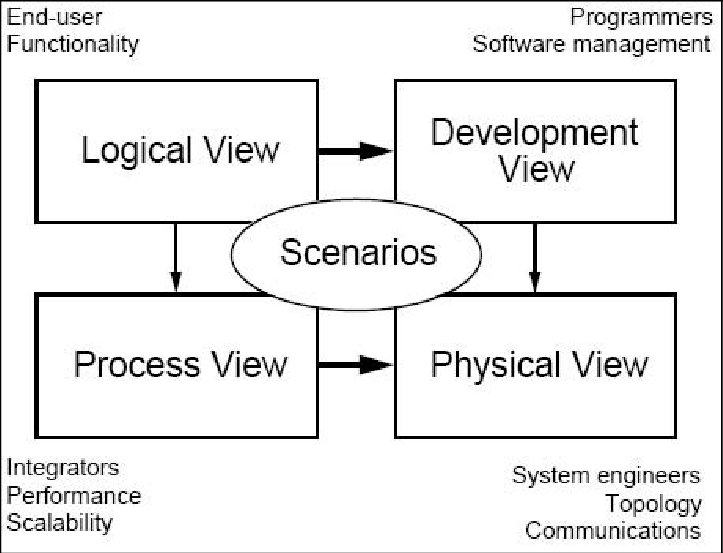
\includegraphics[width=0.6\textwidth]{img/4+1.png}
\end{figure}

\textit{Se puede leer el paper }\href{https://www.cs.ubc.ca/~gregor/teaching/papers/4+1view-architecture.pdf}{aquí}

\subsection*{Vista lógica}
\begin{itemize}
\item Tratar de poner los requisitos funcionales (los relevantes). Se aplican los principios de encapsulamiento y herencia.
\item Diagramas de estados, clases, secuencia y actividad son herramientas que vamos a necesitar en esta vista.
\item Le interesa al usuario final.
\end{itemize}


\subsection*{Vista de desarrollo (o componentes)}
\begin{itemize}
\item Se centra en la organización de los módulos de software en el ambiente de desarrollo del software.
\item Tiene en cuenta los requisitos internos relativos a la facilidad de desarrollo, administración del software, reutilización y elementos comunes, y restricciones impuestas por las herramientas.
\item Usamos diagramas de componentes.
\item Le interesa al desarrollador.
\end{itemize}



\subsection*{Vista procesos}
\begin{itemize}
\item Se centra en requisitos no funcionales tales como rendimiento, disponibilidad, tolerancia ante fallas e integridad.
\item Relacionada con la de componentes.
\item Se usan diagramas de clases
\item Le interesa al diseñador del sistema y al que lo integre.
\end{itemize}


\subsection*{Vista física (o despliegue)}
\begin{itemize}
\item Toma en cuenta los requisitos no funcionales de escalabilidad, performance y disponibilidad.
\item Le interesa al diseñador del sistema.
\end{itemize}


\subsection*{Vista de Escenarios}
\begin{itemize}
\item Para que escenarios estamos planteando nuestra solución. Son una abstracción de los requisitos mas importantes.
\item Le interesa al usuario final.
\item Busca ver el entendimiento del sistema.
\end{itemize}



\section*{Clase 13}
\section{Practica: Normalización II}
\subsection*{Algoritmo de descomposición en 3FN}

Este algoritmo es constructivo, garantiza la preservación de dependencias y la información (por incluir una clave del esquema original)
Entra un esquema R y salen varios Ri en 3FN que preservan información y dependencias funcionales.
\begin{enumerate}
\item Buscamos un conjunto minimal para F
\item Encontramos las claves de R
\item Para cada dependencia funcional $X\rightarrow A_i$ en $F_{min}$ creamos un esquema que tenga a X y a $A_i$.
\item Si ningún esquema de los generados contiene una clave de R, se crea un esquema adicional que contenga atributos que formen una superclave de R. Necesitamos encontrar por lo menos una en las relaciones resultantes.
\item Opcional, pero bueno, es unir los esquemas que tengan la misma clave primaria.
\end{enumerate}

\medskip
Un problema del algoritmo es que puedo fragmentar demasiado, tener muchos esquemas chicos.


% R(ABCDE)
% AB->C , A->D , BD->C
% donde tengo D, puedo poner A
% cc = ABE
% Fmin = A->D, BD->C
% estamos en 1ra forma normal
% lo descomponemos
% R1(AD) A->D
% R2(BCD) BD->C
% R3(ABE) cc=ABE - como la cc no estaba en ninguno creamos una relacion mas, sin esto no sirve la descomposicion


% R4(ABCDEGH)
% Fmin = c->e,g->a,b->d,h->a,h->e,bc->g,acd->g,abe->h,gh->c,gh->b
% cc = bc, beg, cdh, gh
% R1(CE) c->e
% R2(GA) g->a ESTA INCLUIDO EN R7
% R3(BD) b->d
% R4(HA) h->a POSIBLE UNION CON R5
% R5(HE) h->e
% R6(BCG) bc->g <- CLAVE CANDIDATA
% R7(ACDG) acd->g
% R8(ABEH) abe->h
% R9(GHC) gh->c TIENE MISMA CLAVE PRINCIPAL CON R10D
% R10(GHB) gh->b

\subsection*{Algoritmo de descomposición de FNBC}
Tiene la propiedad NJB (comprobación de concatenación no aditiva para descomposiciones binarias) si y solo si la df entre las relaciones R1 y R2 implican la resta de R1 con R2, o R2 con R1 esta en la clausura transitiva de F.

Cuando descomponemos puede pasar que perdamos df. Se garantiza que se mantiene la información por propiedad NJB.

Entra un esquema R y salen varios Ri en FNBC que preservan información.

Vemos en que FN esta, y ahi decidimos si corresponde aplicar el algoritmo.
\begin{enumerate}
\item Establecemos D=$\{R\}$
\item Mientras que exista un esquema Q en D que no este en FNBC
\begin{enumerate}
    \item Escogemos Q en D que no este en FNBC
    \item Encontrar una dependencia funcional $X\rightarrow Y que viole FNBC$
    \item Reemplazamos Q en D por dos esquemas. Un esquema es $R_1 =\{X\}^+ S_1 =proyección S en R_1$ y el otro $R2=\{Q - \{X\}^+ \cup X\} S_2 =proyección S en R_2$
\end{enumerate}
\item Procesar recursivamente R1 y R2
\end{enumerate}

\medskip
El resultado es que se va formando un árbol. Este conviene dibujarlo para no perderse.

Cuando descomponemos puede que perdamos
df’s, pero también puede que en los nuevos
esquemas se puedan representar otras
dependencias que no estén explicitadas en
nuestro conjunto de df´s, pero que
implícitamente existan. Entonces debemos
proyectar nuestro conjunto de df´s en el nuevo
conjunto.

% para el parcial marcar el resultado
% tener bien por lo menos un ej de cada tema

\subsection*{Algoritmo Tableau}
Detecta perdida de información. Lo hace mapeando todas las descomposiciones de R y luego se va operando con las dependencias funcionales para tratar de reconstruir la relación universal. Si podemos reconstruirla no hubo perdida de información. Este método es una simplificación del método Chase

\begin{itemize}
\item Entra una relación, sale un si o un no. 
\item Construimos una matriz con NFIL y NCOL, la columna k corresponde al atributo Aj y la fila i corresponde al esquema Ri de PROY. Los valores de las columnas, para cada una de las filas Ri de la matriz, se rellenan de la siguiente forma:
\begin{itemize}
\item Si Aj está en Ri, MATij=Aj
\item Si Aj no está en Ri, MATij=biAj
\end{itemize}
\end{itemize}

\medskip
Luego vamos aplicando las dependencias funcionales. 
Tenemos que lograr que una fila con todos los atributos.

\medskip
Donde participa cada atributo en las relaciones, pongo las letras correspondientes a esos atributos en la matriz, el resto lo relleno con bij.

\medskip
Aplicamos dependencias, donde tengo mismos valores, tiene que implicar lo mismo, remplazando los valores (priorizamos las mayúsculas). (Queremos lograr una fila con letras mayúsculas) (Si la implicación tiene mas de un atributo de un lado, buscamos esa cantidad, esos pares tienen que ser iguales)

\medskip
No importa el orden en que apliquemos las dependencias, es recursivo, ante cualquier cambio hay que volver a aplicar todas las dependencias. 


\newpage

\section*{Clase 14}
\section{Patrones de diseño}


\begin{itemize}
\item Se nombran solo algunos patrones de diseño, hay un montón. Estos se descubren con el tiempo. Una lista con muchos patrones \href{https://java-design-patterns.com/patterns/}{aquí}.
\item Es buena practica usar nombres que relacionen a los patrones usados.
\end{itemize}

\medskip
\textit{Libro muy recomendado: Design Patterns - Erich Gamma}

\subsection*{Patrones creacionales}
\begin{itemize}
\item Las abstractas arriba, las dependientes - inestables - abajo. Esto muestra la inversión en la cadena de dependencia.
\item Se usan cuando hay que aislar la creación de instancias.
\item Resuelven el encapsulamiento, ocultan y ordenan la creación de instancias, vuelven al sistema independiente del proceso de creación.
\item No publicar cuestiones que no le interesa a otro paquete.
\item Se vuelven mas importantes a medida que se pasa de usar herencia a composición de objetos.
\item Nos dan mucha flexibilidad en cuanto a que se crea, quien lo crea, como es creado, y cuando se crea.
\end{itemize}


\subsubsection*{Factory Method}
\begin{itemize}
\item La forma más simple de ocultar la creación de un objeto es usando un método que devuelve un objeto.
\item Si aparecen nuevas clases del tipo1, extendemos la de la fabrica original, de manera tal de ocultar la creación de cada uno de los tipos en métodos de las clases diferentes.
\item Presenta la dificultad de mantener 2 jerarquías de clases en paralelo.
\item Se bautiza como factory method a cualquier clase que tenga un método para crear otro objeto y devolverlo.
\item Su intención es crear una interfaz para la creación de un objeto que permita a las subclases decidir que clase instanciar.
\item Elimina la necesidad de atar clases especificas de la aplicación al código.
\item Crear en una manera descriptiva las instancias los que no son descriptivos. (\textit{Clase con muchos constructores, se complica elegir cual. Necesitamos sacar la ambigüedad de esto. Una forma de arreglar esto es proveer métodos de clase que tengan nombres descriptivos y constructores protegidos. Cada uno de los métodos seria un factory method. (no es la version propuesta por Gamma, es valida igual. )}) - \href{https://github.com/brunograssano/Algoritmos_3_TP2_PM2/blob/master/src/main/java/edu/fiuba/algo3/modelo/preguntas/FabricaDePreguntas.java}{Ejemplo}
\end{itemize}

\begin{figure}[!htb]
    \centering
    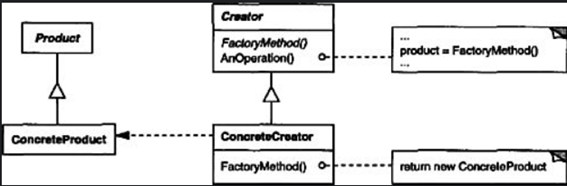
\includegraphics[width=0.8\textwidth]{img/FactoryMethod.png}
\end{figure}

\subsubsection*{Abstract Factory}
\begin{itemize}
\item Logramos un esquema en el cual se crean objetos concretos sin violar la inversión de la dependencia.
\item Busca proveer una interfaz para crear familias de objetos relacionados o dependientes entre si sin especificar la clase en concreto.
\item Se usa cuando un sistema debe de ser independiente de como se crean los objetos, cuando un sistema debe de configurarse con una familia de objetos de muchas.
\item Aísla las clases concretas. Los clientes interactúan solo con la interfaz.
\item Vuelve fácil el cambio de productos de familias.
\item Promueve consistencia entre los productos.
\item Se vuelve difícil soportar nuevos tipos de productos. Esto es porque la interfaz de la abstract factory fija el conjunto de productos.
\end{itemize}

\begin{figure}[!htb]
    \centering
    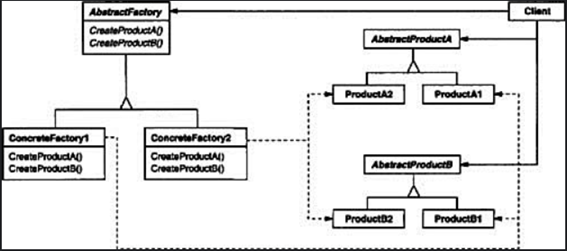
\includegraphics[width=0.8\textwidth]{img/AbstractFactory.png}
\end{figure}

\subsubsection*{Prototype}
\begin{itemize}
\item En vez de crear clona objetos. Nos evita tener que mantener la jerarquía paralela de la factory. (Variante del Abstract Factory)
\item La intención es especificar los tipos de objetos a crear a partir de un prototipo, y crear nuevos objetos a partir de copiar el prototipo.
\item Se usa cuando un sistema debe de ser independiente de como sus productos son creados, las clases de productos a instanciar se especifican en tiempo de ejecución, se quiere evitar jerarquías de fabricas paralelas a la de productos,  las instancias de una clase solo pueden tener pocas combinaciones de estado..
\item Esto esconde las clases concretas del cliente.
\item Se pueden agregar y quitar prototipos en tiempo de ejecución.
\item Reduce las subclases
\end{itemize}

\begin{figure}[!htb]
    \centering
    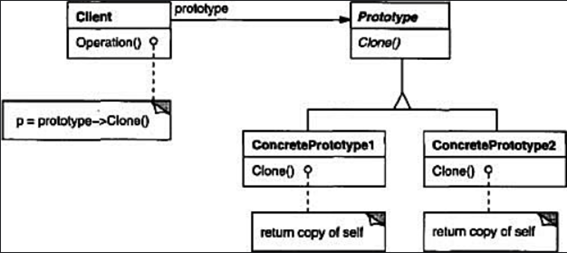
\includegraphics[width=0.8\textwidth]{img/Prototype.png}
\end{figure}

\subsubsection*{Builder}
\begin{itemize}
\item Variante del abstract factory. Cuando invoco a crear un objeto, invoca a la creación de cada parte del objeto complejo.
\item Busca separar la construcción de un objeto complejo de la representación, de forma tal de que el mismo proceso cree diferentes representaciones.
\item Se usa cuando el algoritmo de creación deba de ser independiente del objeto y la construcción deba de permitir diferentes representaciones.
\item Esto permite cambiar la representación interna de un producto y esconde la representación interna del producto con la interfaz.
\item Aísla el código para construcción y representación. Esto mejora la modularidad al encapsular el proceso.
\item Nos da un control mas fino sobre el proceso de creación. (Lo hace al objeto paso a paso)
\end{itemize}

\begin{figure}[!htb]
    \centering
    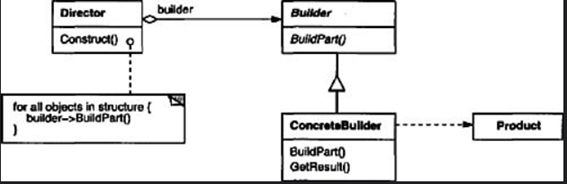
\includegraphics[width=0.8\textwidth]{img/Builder.png}
\end{figure}

\begin{figure}[!htb]
    \centering
    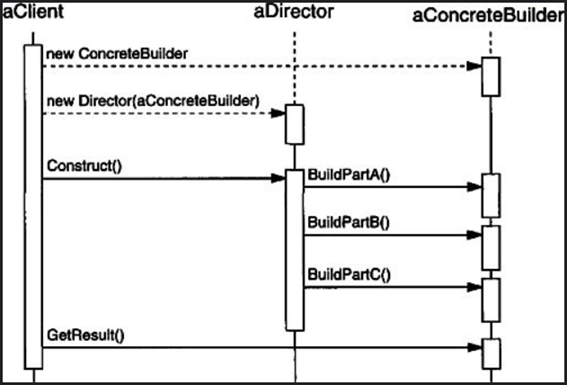
\includegraphics[width=0.8\textwidth]{img/Builder2.png}
\end{figure}

\subsubsection*{Singleton}
\begin{itemize}
\item Se usa cuando se quiere que exista una única instancia de una clase y proveer un único punto de acceso a ella.
\item Permite un punto de accesos controlado.
\item Es una mejora respecto de variables globales. (En cierta forma lo es todavía)
\item Permite variar el numero de instancias.
\item Es mas flexible que métodos de clase.
\item Se puede extender la clase.
\item Los usos mas frecuentes son en caches, configuraciones y pulls.
\end{itemize}

\begin{figure}[!htb]
    \centering
    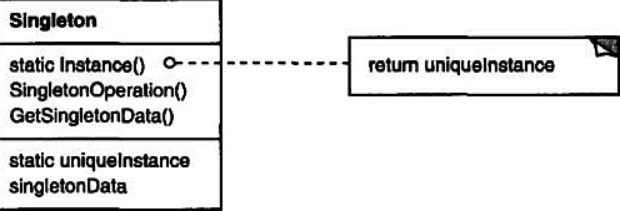
\includegraphics[width=0.8\textwidth]{img/Singleton.jpg}
\end{figure}


\subsection*{Patrones de organización del trabajo - Behavioral Patterns}
\begin{itemize}
\item Estos patrones conviene usarlos cuando hay que repartir las responsabilidades entre objetos.
\end{itemize}


\subsubsection*{Command}
\begin{itemize}
\item La intención es encapsular la acción de un objeto.
\item Se usa cuando se quiere parametrizar objetos mediante una acción a ejecutar, especificar, encolar, y ejecutar acciones en diferentes momentos, soportar deshacer la operación.
\item Desacopla el objeto que solicita un servicio de aquel que lo presta. Versión en objetos de una función Callback
\item Se pueden componer comandos con un composite.
\item Se vuelve fácil agregar nuevos comandos, no se tiene que cambiar clases existentes.
\end{itemize}


\begin{figure}[!htb]
    \centering
    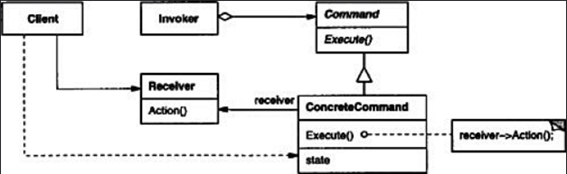
\includegraphics[width=0.8\textwidth]{img/Command.png}
\end{figure}

\subsubsection*{Chain of Responsability}
\begin{itemize}
\item La intención es desacoplar quien envía un mensaje de quien lo ejecuta. Los objetos lo van pasando.
\item Se usa cuando mas de un objeto puede manejar un mensaje y este objeto no se conoce a priori, se quiere mandar un mensaje a varios objetos sin especificar cuales en especifico, el conjunto de objetos que manejan el mensaje se especifica dinámicamente.
\item Va pasando la posta hasta que lo trate alguien. Desacoplar quien solicita un servicio de un conjunto.
\item Se puede ver también como una función de orden superior que toma una función, y si no puede resolver lo delega a la función.
\item Reduce el acoplamiento. Libera a los objetos del saber quien lo va a manejar al mensaje.
\item Da flexibilidad en asignar responsabilidades a los objetos.
\item El receptor no esta garantizado, por lo que puede no ejecutarse si no se configura correctamente.
\end{itemize}

\begin{figure}[!htb]
    \centering
    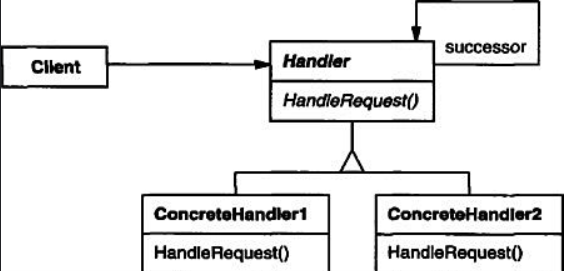
\includegraphics[width=0.8\textwidth]{img/ChainOfResponsability.png}
\end{figure}

\subsubsection*{Mediator}
\begin{itemize}
\item La intención es definir un objeto que encapsule como un conjunto de objetos interactúan.
\item Se usa cuando un conjunto de objetos se comunican de forma bien definida pero compleja.
\item Busca evitar una cantidad de dependencias enormes entre todos los componentes. Este mediador elimina las dependencias cruzadas, pero tiene la desventaja de que todos conocen al mediador, y que el mediador conoce a todos (Tenemos una dependencia circular). Es fácil agregar componentes adicionales porque la lógica esta concentrada en el mediador.
\item Limita las subclases. Localiza todo el comportamiento que estaría distribuido.
\item Desacopla los collegues.
\item Vuelve mas abstracto como cooperan los objetos.
\item Centraliza el control.
\item No es necesario definir la clase abstracta mediator en la implementación.
\end{itemize}

\begin{figure}[!htb]
    \centering
    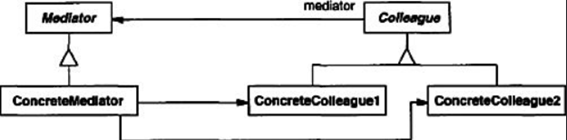
\includegraphics[width=0.8\textwidth]{img/Mediator.png}
\end{figure}

\begin{figure}[!htb]
    \centering
    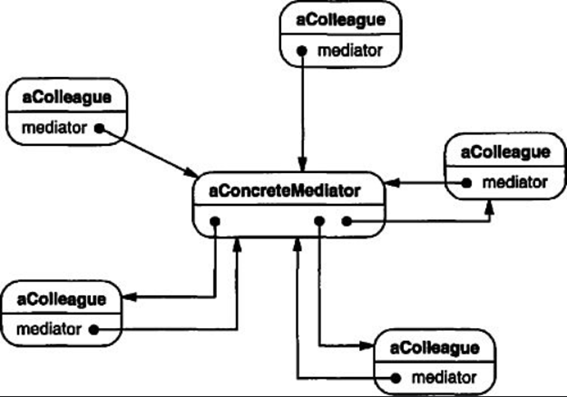
\includegraphics[width=0.6\textwidth]{img/Mediator2.png}
\end{figure}

\subsection*{Patrones de control de acceso}

\begin{itemize}
    \item Se encargan sobre como las clases y objetos se componen para formar estructuras mas grandes. (Structural Patterns)
    \item Compone objetos para lograr nuevas funcionalidades. (Structural Patterns)
\end{itemize}

\subsubsection*{Facade (Structural Patterns)}
\begin{itemize}
\item La intención es proveer una interfaz unificada a un conjunto de interfaces de un subsistema.
\item Se usa cuando queremos una interfaz simple a un subsistema complejo, hay muchas dependencias entre clientes y la implementación de las clases de una abstracción, queremos una capa entre los subsistemas (entry point).
\item Escribimos código para acceder servicios externos y no contaminar el contexto de nuestro sistema. Aparece la segregación de interfaces.
\item Tener un acceso de mas alto nivel.
\item Reducir el acoplamiento.
\item Protege a los clientes de las componentes de los subsistemas.
\item Promueve weak coupling entre los subsistema y los clientes.
\item No previene a las aplicaciones el uso de los subsistemas si quieren. Permite elegir entre la facilidad de uso y la generalidad.
\end{itemize}

\begin{figure}[!htb]
    \centering
    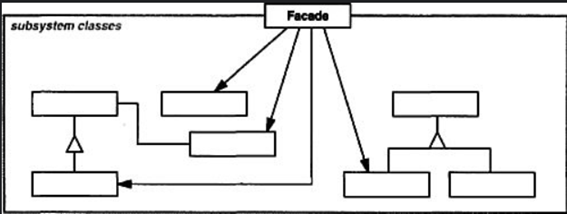
\includegraphics[width=0.8\textwidth]{img/Facade.png}
\end{figure}

\begin{figure}[!htb]
    \centering
    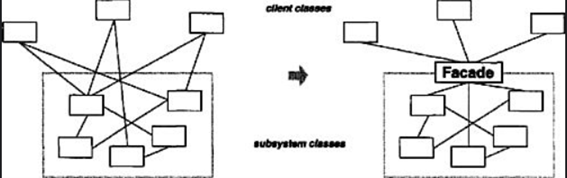
\includegraphics[width=0.8\textwidth]{img/Facade2.png}
\end{figure}

\subsubsection*{Proxy (Structural Patterns)}
\begin{itemize}
\item Su intención es proveer un sustituto a otro objeto para controlar el acceso.
\item En los métodos de proxy se decide que puede hacer la clase que llama respecto de la clase oculta.
\item Controla acceso a determinados tipos de recursos, esto posterga el costo de la creación e inicialización hasta que se necesite.
\item Proxy remoto para objetos separados de lugar.
\item Proxy virtual: Se usa en las arquitecturas de tipo EA. Lazy load, creo en memoria un proxy, el cliente se cree que tiene un objeto completo, pero en realidad voy trayendo lo que necesito a medida que se pide.
\item El proxy dio lugar al garbage collector, de alguna manera controla la creación y destrucción de objetos.
\end{itemize}

\begin{figure}[!htb]
    \centering
    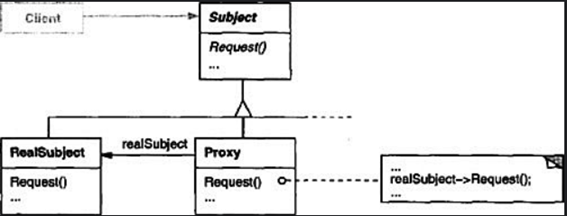
\includegraphics[width=0.8\textwidth]{img/Proxy.png}
\end{figure}

\subsubsection*{Iterator (Behavioral Patterns)}
\begin{itemize}
\item La motivación es proveer una forma de acceder a los elementos de un aggregate object se forma secuencial sin exponer la representación.
\item Permite múltiples formas de recorrer el objeto.
\item Provee una interfaz uniforme para el recorrido. (polymorphic iteration)
\item Sirve para no exponer los datos de una colección directamente, los accedo a través de un iterador.
\end{itemize}

\begin{figure}[!htb]
    \centering
    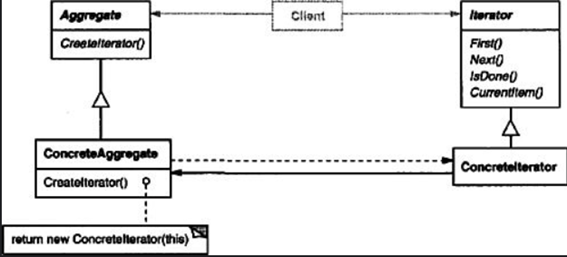
\includegraphics[width=0.8\textwidth]{img/Iterator.png}
\end{figure}


\subsection*{Variación de servicio}
Quiero resolver que objetos de determinadas clases tengan un comportamiento distinto.


\subsubsection*{Strategy (Behavioral Patterns)} 
\begin{itemize}
\item Se usa cuando tengo muchas formas de hacer una cosa. Se dice que encapsula un algoritmo y permite variarlo independientemente de los clientes..
\item Cambia el algoritmo completo.
\item Recibe el contexto que es la clase que se va a usar. Contiene la información necesaria para resolver la estrategia.
\item Se aprovecha en tiempo de ejecución.
\item De acuerdo a la estrategia que use estoy variando lo que hago.
\end{itemize}


\begin{figure}[!htb]
    \centering
    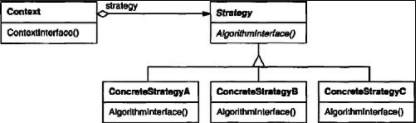
\includegraphics[width=0.8\textwidth]{img/Strategy.PNG}
\end{figure}


\subsubsection*{Template Method}
\begin{itemize}
\item El algoritmo esta prefijado, el esqueleto de este.
\item Cada una de las clases redefinen el paso correspondiente.
\item El objeto instanciado ejecuta el algoritmo.
\item Muy usado en los frameworks.
\item Se trata de tener diversidad y resolverlo en tiempo de compilación.
\item Variación de servicio en tener la posibilidad al instanciar un objeto de variar los pasos.
\item Fundamental para reusar código.
\end{itemize}


\begin{figure}[!htb]
    \centering
    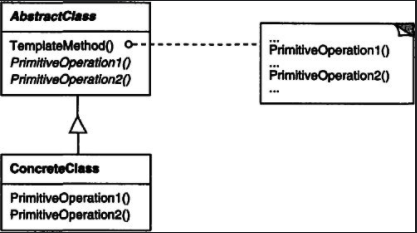
\includegraphics[width=0.5\textwidth]{img/TemplateMethod.PNG}
\end{figure}

\subsubsection*{State (Behavioral Patterns)}
\begin{itemize}
\item Tiene que ver con que los objetos se comporten de acuerdo al estado en que están.
\item El estado de un objeto depende de su historia. Desde que lo inicializamos.
\item Un indicativo de usar el patrón es cuando aparecen muchas condiciones.
\item Maquina de estados para realizar los cambios sin que se conozcan entre si los estados. Usa una lookup table que conoce a todos los estados concretos.
\item Puede tener un contexto que le pase lo que necesita al estado, o incluso pasarse a si mismo.
\item Como resultado del patrón, se ubica el comportamiento especifico en diferentes particiones para cada estado. (Puede llegar a introducir muchas clases, sin el patrón se tendrían condicionales)
\end{itemize}


\begin{figure}[!htb]
    \centering
    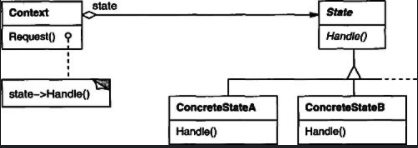
\includegraphics[width=0.8\textwidth]{img/State.PNG}
\end{figure}

\subsection*{Extensión de servicio}
Quiero que los objetos de mi clase hagan lo que hacían y algo mas.

\subsubsection*{Decorator}
\begin{itemize}
\item Esta orientado a objetos 'livianos'. Que encapsulen comportamiento más que atributos.
\item El decorador extiende el servicio en tiempo de ejecución, le agrega o quita responsabilidades. (dinámico)
\item Decorador puede tener clases hijas que redefinan su comportamiento.
\item Es mucho más flexible que la herencia.
\item Podemos decorar múltiples veces el mismo objeto. (a objetos individuales, no a clases enteras)
\item Da mucha reusabilidad.
\item Generalmente se usa con Composite.
\item Un sistema que usa Decorator generalmente termina lleno de un montón de objetos pequeños que se parecen entre si.
\end{itemize}


\begin{figure}[!htb]
    \centering
    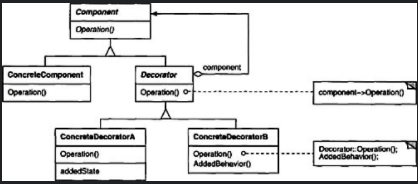
\includegraphics[width=0.8\textwidth]{img/Decorator.PNG}
\end{figure}

\subsubsection*{Visitor}
\begin{itemize}
\item Lo usamos para agregar métodos/funciones a una clase.
\item Se dice que es un double dispatch.
\item Representa una operación que se ejecuta en los elementos de una estructura. Permite crear esta operación sin tener que cambiar las clases de los elementos. en los que opera.
\item Se puede usar cuando un objeto contiene muchas clase de objetos con diferentes interfaces y queremos realizar acciones que dependen de las clases concretas.
\end{itemize}


\begin{figure}[!htb]
    \centering
    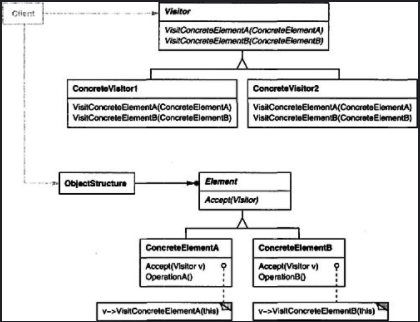
\includegraphics[width=0.8\textwidth]{img/Visitor.PNG}
\end{figure}

\subsection*{Varios}

\subsubsection*{Bridge}
Cuando se deba desacoplar abstracciones de implementaciones
Los métodos de las abstracciones delegan en las implementaciones
Se complementa con algún patrón creacional.
Cambios en la implementación de una abstracción no debería de impactar a los clientes.
Oculta detalles a los clientes.
Se puede extender fácilmente.

\begin{figure}[!htb]
    \centering
    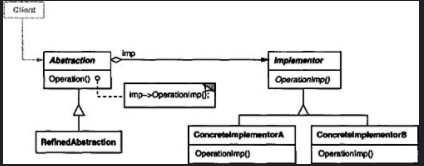
\includegraphics[width=0.8\textwidth]{img/Bridge.PNG}
\end{figure}

\subsubsection*{Adapter}
\begin{itemize}
\item Esta orientado a reutilizar código.
\item Cuando es necesario adaptar una clase para que funcione en el contexto que necesito.
\item Suele usarse para adaptar los métodos de algún sistema externo que estamos usando para que un facade acceda a ese sistema.
\item Convierte una interfaz en otra que espera el cliente.
\item Se pueden usar Adapters de dos direcciones para agregar transparencia (generalmente no son transparentes a todos los clientes)
\end{itemize}


\begin{figure}[!htb]
    \centering
    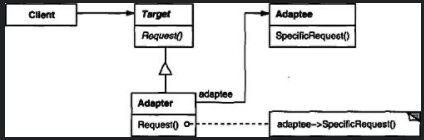
\includegraphics[width=0.8\textwidth]{img/Adapter.PNG}
\end{figure}

\subsubsection*{Composite}
\begin{itemize}
\item Esta orientado a ofrecerle al cliente una misma interfaz para que un objeto se trate de un único objeto o una colección de objetos.
\item Ejemplos de uso se ven en procesamiento de texto y filtros.
\item Compone objetos en estructuras - similares a arboles - para representar jerarquías.
\item Como se vuelve indistinguible al grupo de objetos de un solo objeto, simplifica al cliente. Esto trae una desventaja también, si el diseño se vuelve muy general se complica agregar restricciones a los componentes del composite.
\item Para maximizar esta indistinguibilidad, se debe de agregar la mayor cantidad posible de métodos comunes en la interfaz. (Puede llevar a entrar en conflicto con la separación de lo que corresponde a cada clase)
\end{itemize}


\begin{figure}[!htb]
    \centering
    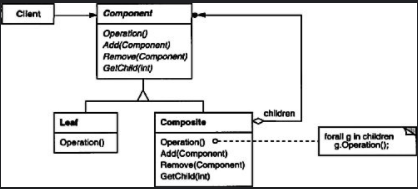
\includegraphics[width=0.8\textwidth]{img/Composite.PNG}
\end{figure}

\section*{Clase 15}
\section{Bases de datos espaciales}
\begin{itemize}
\item Tenemos que ver las distorsiones que ocurren al pasar de un mapa geoide al plano. Introducción al tema de geodesia \href{https://www.ign.gob.ar/NuestrasActividades/Geodesia/Introduccion}{aquí}
\item Las bases de datos espaciales (llamadas también geográficas) permiten representar en forma eficiente objetos definidos en un espacio geométrico. 
\item Tienen 3 objetos simples (puntos, lineas, polígonos) y 2 complejos (objetos 3D, teselados).
\item Son parte de un contexto más general, los sistemas de información geográfica GIS que permite almacenar y manipular datos geográficos y capturar, analizar y presentar visualmente datos geográficos.
\end{itemize}


\subsection*{Representaciones}
Tenemos 2 representaciones posibles:

\begin{itemize}
\item En las representaciones vectorizadas los objetos se identifican con vectores que identifican los bordes. Tiene un alto nivel de detalle y es fácil de mantener y actualizar, pero tiene una pobre representación de datos continuos.
\item En las rasterizadas los objetos se proyectan sobre una matriz de celdas. Se pueden representar datos continuos (Ej. elevación), se puede hacer un análisis cuantitativo de forma fácil, es fácil de renderizar. La desventaja es que el detalle depende de la resolución y que suelen ocupar mas espacio.
\end{itemize}

En general se trabaja con los dos tipos de imágenes juntas. (basemap) (Ej, poner un camino de GPS arriba de una imagen satelital.)

\begin{figure}[htb]
    \centering
    \includegraphics[width=0.7\textwidth]{img/RepresentacionesImagenes.PNG}
\end{figure}


\subsection*{Simple Features}

\begin{itemize}
\item Define una representación textual estándar para los objetos genéricos. Se conoce como WKT (Well Known Text). Hay otra que es Well Known Binary Representation (WKB)
\item Define cómo agregar funcionalidad espacial a las bases de datos a través de una representación vectorizada, especificando con notación UML.
\end{itemize}

\begin{figure}[htb]
    \centering
    \includegraphics[width=0.7\textwidth]{img/SistemaGraficoBasesEspaciales.PNG}
\end{figure}

\begin{itemize}
\item Sistema de coordenadas (spatial reference system) SRID, usamos el 4326 en el taller (usado por el sistema GPS)
\item spatial\_ref\_sys tiene los sistemas referenciales que podemos usar.
\item Para buscar y combinar objetos geograficos se utilizan estructuras eficientes. Por ejemplo kd-trees o R-trees.
\end{itemize}


\subsection*{Taller}

\begin{itemize}
\item Creamos base de datos, vamos a extensiones. Creamos una extensión postgis y otra postgis\_raster. Luego creamos las tablas, las importamos desde el postgis.
\item Nos conectamos con la base de datos e importamos los archivos poniendo el SRID en la columna. Una vez que lo hacemos seleccionamos importar.
\item Hacemos el refresh de las tablas en la base de datos y ya podemos ver los datos.
\item Stack Builder para instalar paquetes al postgres.
\item QGis para las imágenes satelitales, instalamos el complemento y vamos a administrar base de datos donde importamos el archivo de la imagen satelital.
\end{itemize}

\begin{minted}
[
frame=leftline,
framesep=5mm,
baselinestretch=1.2,
]
{sql} 
SELECT gid, nombre_est, comuna, barrio, geom
FROM primarias
WHERE gid IN (2808, 1191, 190, 559, 1512)
\end{minted}

\subsubsection*{Obtener el área de todas las comunas expresada en hectáreas}
\begin{minted}
[
frame=leftline,
framesep=5mm,
baselinestretch=1.2,
]
{sql}
SELECT comunas, area, ST_Area(geom::GEOGRAPHY)/10000 AS area_en_ha
FROM comunas
ORDER BY 1;
\end{minted}

No esperar encontrar geometrías exactas, puede no dar lo mismo que el valor que se tiene al calcular el área.


\subsubsection*{¿Hay barrios que sean iguales a comunas? ¿Cuales?}
Vemos si hay polígonos iguales.
\begin{minted}
[
frame=leftline,
framesep=5mm,
baselinestretch=1.2,
]
{sql} 
SELECT c.comunas, c.geom
FROM barrios AS b, comunas AS c
WHERE st_equals(c.geom, b.geom)
ORDER BY 1 ASC
\end{minted}

Hay 3 en realidad pero da 1 debido a los errores en el calculo. Si queremos los otros 2 hay que 'perdonar' la superposición.

\subsubsection*{Visualice la comuna 1 dentro del entramado de barrios}
Ejemplo de unión de los barrios con la comuna.
\begin{minted}
[
frame=leftline,
framesep=5mm,
baselinestretch=1.2,
]
{sql} 
SELECT st_union(c.geom, b.geom)
FROM comunas c, barrios b
WHERE c.comunas=1
\end{minted}

\subsubsection*{Calcule la distancia entre todas las escuelas}
\begin{minted}
[
frame=leftline,
framesep=5mm,
baselinestretch=1.2,
]
{sql} 
SELECT p1.nombre_est, p2.nombre_est, ST_DistanceSphere(p1.geom,p2.geom)
FROM primarias AS p1, primarias AS p2
WHERE p1.gid < p2.gid
ORDER BY 3 DESC
\end{minted}


\subsubsection*{Obtenga un ranking de las escuelas más aisladas}
\begin{minted}
[
frame=leftline,
framesep=5mm,
baselinestretch=1.2,
]
{sql} 
SELECT grid_1, estab_1, min(dist) AS distMin
FROM distancias AS p1
GROUP BY 1, 2
ORDER BY 3 DESC
\end{minted}


\subsubsection*{Muestre las escuelas primarias y los radios censales}
\begin{minted}
[
frame=leftline,
framesep=5mm,
baselinestretch=1.2,
]
{sql} 
SELECT p.geom
FROM primarias AS p
UNION
SELECT c.geom
FROM censo_2010_cada AS c
\end{minted}

Escuelas en comuna 1 mostrando radios censales
\begin{minted}
[
frame=leftline,
framesep=5mm,
baselinestretch=1.2,
]
{sql} 
SELECT p.geom
FROM primarias AS p
WHERE p.comuna = 1
UNION
SELECT ST_union(p.geom, c.geom)
FROM primarias AS p, censo_2010_cada AS c
WHERE p.ST_Within(p.geom, c.geom) AND p.comuna = 1
\end{minted}


\section*{Clase 16 y 18}
En realidad se extendió mas clases el tema.
\section{NoSQL}

\begin{itemize}
\item No responden al modelo relacional.
\item Surgen alrededor de los 2000 con la masificación de la Web y cambios tecnológicos.
\item Necesidades de almacenar muchos datos. (Google, Amazon)
\item Se tenían requerimientos
\item Mayor escalabilidad para trabajar con grandes volúmenes de datos.
\item Mayor performance en aplicaciones Web. Surge XML y JSON, formatos fáciles de serializar y procesar.
\item Mayor flexibilidad sobre las estructuras de datos. Los SGBD relacionales son muy rígidos, agregar una columna puede ser muy costoso.
\item Mayor capacidad de distribución. Viene de la mano con escalabilidad. Se busca mayor disponibilidad y tolerancia a fallas de parte del SGBD.
\end{itemize}

\medskip
Los SGBD relacionales tiene limitaciones en cuanto a los joins de tablas, son costosos y el manejo de transacciones en forma distribuida no escala (Se vuelve difícil garantizar ACID cuando tenemos muchos nodos).

\medskip
Lectura sugerida: \href{https://www.enterpriseintegrationpatterns.com/ramblings/18_starbucks.html}{Starbucks Does Not Use Two-Phase Commit}

\medskip

Se tenían redes cada vez mas rápidas, almacenamiento mas barato, pero velocidad de procesamiento estancada. Se pueden revisar los números del cambio \href{https://colin-scott.github.io/personal_website/research/interactive_latency.html}{aquí}. Debido a esto surge la necesidad de bases de datos distribuidas.

\medskip
Las bases de datos NoSQL buscan aumentar la velocidad de procesamiento y la capacidad de almacenar información. Para ello implementan un sistema de gestión de bases de datos distribuido.

\bigskip
Para hablar de las bases de datos no sql se necesitan algunos conceptos:

\begin{itemize}
\item \textbf{Fragmentación}: repartimos el contenido en muchos nodos. En uno solo no nos entra. Es la tarea de dividir un conjunto de agregados entre un conjunto de nodos. Puede ser fragmentación horizontal (los agregados se reparten entre los nodos de manera que cada nodo almacena un subconjunto de agregados. Se asigna el nodo a partir del valor de alguno de los atributos del agregado) o vertical ( Distintos nodos guardan un subconjunto de atributos de cada agregado. Todos suelen compartir los atributos que conforman la clave - no es lo mas común) (En un solo nodo no nos entra, toma mucho tiempo)
\item \textbf{Replicación}: si se cae uno que lo pueda manejar otro. Tiene varias ventajas, provee backup, repartir la carga de procesamiento, y garantizar la disponibilidad del sistema si se caen algunos nodos. El problema que genera es la consistencia de los datos. Cuando se usan solo como backup se dice replica secundaria. Cuando pueden hacer procesamiento también se conoce como replica primaria. La replica introduce el problema de consistencia, que un mismo item de datos tenga el mismo valor en todas las replicas. (A prueba de fallas)
\item \textbf{Búsqueda (lookup)}: saber donde esta lo que necesito, que nodo tiene determinado dato. No esta este problema en una base de datos relacional. Se usan tablas de hash distribuidas.
\item \textbf{Métodos de consistencia}: Que pasa si un mismo dato tiene valor distinto en distintos nodos. Puede suceder cuando los usuarios están modificando los datos. Tiene que haber una forma de controlar esto, que los usuarios se pongan de acuerdo o no pase. Surge por la replicación,
\item \textbf{Métodos de acceso (Access method)}: Como llego dentro del nodo a la información que quiero de forma rápida. (LSM Trees y estructuras) diferenciales)
\end{itemize}



\subsection*{Clasificación}
\subsubsection*{Clave-Valor}

\begin{itemize}
\item Almacenan vectores asociativos o diccionarios, es decir pares.
\item Las claves son únicas (no puede haber 2 pares con la misma clave).
\item Ejemplos son Dynamo y Redis.
\item Operaciones: PUT un nuevo par, UPDATE par de la clave, DELETE par de la clave, GET par de la clave
\item Las ventajas que tienen son: son simples, veloces (eficiencia de acceso sobre la integridad), y escalables (se provee replicación y se pueden repartir las consultas entre nodos).
\item El objetivo es consultar y guardar grandes cantidades de datos.
\end{itemize}

\bigskip
\textbf{Dynamo}\\
\begin{itemize}
\item Es el key-value de Amazon
\item Esta orientada a una arquitectura orientada a servicio (SoA)
\item La base de datos esta distribuida en un server cluster que posee servidores web, routers de agregación y nodos de procesamiento
\item Para consistencia usa un modelo llamado consistencia eventual. Tolera pequeñas inconsistencias (valores distintos).
\item De lookup usa un método de hashing consistente que reduce la cantidad de movimientos de pares necesarios cuando cambia la cantidad de nodos S. Hace que agregar nodos sea sencillo con un impacto mínimo.(no tiene nada que ver con la consistencia, solo minimiza la cantidad de movimientos)
\item La función de hash consistente a partir de una clave $k$ devuelve un valor $h(k)$ entre 0 y $2^M -1$ en donde M representa la cantidad de bits del resultado (hashing). Este valor para un par representa en que nodo se almacena (tabla de hash distribuida)
\item Al identificador de cada nodo de procesamiento (generalmente, su dirección IP) se le aplica la misma función de hash. Los nodos se van organizando virtualmente en una estructura de anillo por hash creciente. (para que si se cae alguno no reorganiza todo, si se cae alguno, el nodo siguiente se ocupa de los datos del nodo que se cayo)
\item Los nodos tienen un listado de preferencia, indica cuales nodos va a replicar. Si se cae un nodo, otro nodo que no esta en este listado va a recibir los datos para mantener (el único movimiento que hay)
\end{itemize}


\subsubsection*{Orientadas a Documentos}

\begin{itemize}
\item Un documento es un agregado, la unidad estructural que contiene la información. 
\item No tenemos un esquema rígido (columnas).
\item Un agregado es un conjunto de objetos relacionados que se agrupan en colecciones para ser tratados como unidad y ser almacenados en un mismo lugar. \textit{Un post de FB con sus comentarios}
\item Generalmente se representan con JSON, XML, YAML...
\item Ejemplos son MongoDB, RavenDB...
\end{itemize}


\bigskip
\textbf{MongoDB}\\
\begin{itemize}
\item Se basa en hashes para identificar los objetos.
\item No usa esquemas pero se le pueden definir.
\item Documentos son JSON.
\item Organiza los datos de una base de datos en colecciones que contienen documentos.
\item No esta pensado para operaciones de junta, en general se pone todo junto en los documentos.
\item La agregación se implementa con un pipeline, uno va definiendo las operaciones a realizar en el. La salida de uno es la entrada de otro.
\item Sharding es el modelo distribuido de procesamiento. Se basa en el particionamiento horizontal de las colecciones en chunks que se distribuyen en nodos llamados Shards. La idea de estos es que estén descentralizados.
\end{itemize}

El esquema de MongoDB se puede ver como:
\begin{figure}[!htb]
    \centering
    \includegraphics[width=0.7\textwidth]{img/MongoDB.PNG}
\end{figure}


\begin{itemize}
\item Son los shards (fragmentos) que se distribuyen los chunks, los routers que reciben las consultas, y los servidores de configuración sobre los shards y routers.
\item Mongo usa para particionar las colecciones una shard key. Es un atributo o conjunto de atributos.
\item Es posible tener colecciones sharded y otras unsharded. Las unsharded se almacenan en un shard particular del cluster. (El shard primario)
\item No es posible desfragmentar una colección ya fragmentada.
\item Usar el sharding permite disminuir el tiempo de respuesta en sistemas con alta carga de consultas al distribuir el procesamiento entre varios nodos y ejecutar consultas sobre conjuntos de datos muy grandes. El objetivo es que la base de datos sea escalable.
\item MongoDB nos permite que cada shard este replicado. Nos sirve para backup y responder consultas.
\item El esquema de replicas es de master-slave with automated failover. Las replicas eligen entre si un master con un algoritmo distribuido. Si el master falla los slaves elijen a un nuevo master.
\item Todas las operaciones de escritura se hacen sobre el master. Los slaves están como respaldo.
\item Los clientes pueden especificar para mandar las consultas de lectura a los nodos secundarios.
\item Durante operaciones de agregación, se puede dar el caso de que los nodos realice operaciones de forma paralela, y cuando no se pueda seguir de forma paralela (se necesita la información de los otros nodos) se le pasan al router para que lo termine la operación.
\end{itemize}


\subsubsection*{Wide Column}

\begin{itemize}
\item Evolución de las bases de datos de clave/valor.
\item Un valor particular de la clave primaria junto con todas sus columnas asociadas forma un agregado análogo a la fila de una tabla. Pero además, estas bases permiten agregar conjuntos de columnas en forma dinámica a una fila, convirtiéndola en un agregado llamado fila ancha (wide row, el nombre quedo como wide column)
\item Ejemplos son Google BigTable, Apache Cassandra...
\end{itemize}

\bigskip
\textbf{Cassandra}\\
\begin{itemize}
\item No es estrictamente orientada a columnas.
\item Usa esquemas.
\item Tiene una arquitectura de share-nothing, no hay un estado compartido centralizado, todos los nodos son pares. Permite que sea muy escalable.
\item Optimizado para ofrecer una alta tasa de escrituras.
\item Cada columna es un par clave-valor asociado a una fila.
\item Cada esquema puede estar distribuido en varios nodos.
\item Es obligatorio definir una clave primaria.
\item Cuando en una fila las columnas se repiten identificadas por el valor que toman las columnas clave, se dice que la fila se convirtió en una wide row (fila ancha).
\end{itemize}

\begin{figure}[!htb]
    \centering
    \includegraphics[width=0.7\textwidth]{img/EsquemaCassandra.PNG}
    \caption{Esquema simple de Cassandra}
\end{figure}

\begin{figure}[!htb]
    \centering
    \includegraphics[width=0.7\textwidth]{img/EsquemaWideRow.PNG}
    \caption{Esquema con Wide Row}
\end{figure}

\begin{itemize}
    \item La clave primaria se divide entonces en clave de partición y de clustering. (La primaria permite identificar a la fila todavía)
    \item Toda la wide-row se almacenara contigua en disco y la clave de clustering nos determina el ordenamiento interno de las columnas.
    \item Restricciones sobre la clave primaria: los valores deben ser comparados por igual contra valores constantes en los predicados, si una columna que forma parte de una clustering key es usada como predicado, deben usarse las restantes columnas también.
    \item No existe el concepto de junta.
    \item No existe el concepto de integridad referencial.
    \item Hay que pensar de antemano que consultas se van a realizar para diseñar las tablas. Se busca que cada consulta se resuelva accediendo a una unica column family, que los resultados esten en una unica particion, respetar las reglas del uso de la clave primaria.
    \item Usa una estructura LSM-Tree que mantiene parte de los datos en memoria para diferir cambios sobre el indice en disco.
    \item Se busca acceder en forma secuencial al disco.
\end{itemize}

\subsubsection*{Basadas en grafos}
\begin{itemize}
\item Los elementos principales son nodos y arcos (ejes)
\item Estas bases resultan útiles para modelar interrelaciones complejas entre las entidades.
\item Mantienen una referencia a sus nodos adyacentes.
\item Se almacena como una lista de adyacencias
\item Sirve para encontrar un patrón de nodos conectados entre si, un camino entre nodos, la ruta mas corta, calcular medidas de centralidad asociadas a los nodos.
\end{itemize}


\bigskip
\textbf{Neo4j}\\
\begin{itemize}
\item Tiene soporte para ACID
\item Formada por nodos que pueden tener distintos labels. 
\item Dentro de cada label el nodo tiene un conjunto de propiedades. Esta estructura no es rígida.
\item Los ejes son siempre direccionales, si se quiere trabajar con no dirigidos no se crean las interrelaciones en ambos sentidos.
\item Un patrón (pattern) puede especificarse a través de un nodo y sus propiedades, una interrelación y sus propiedades, o un camino y sus propiedades. A cada patrón podemos darle un nombre. 
\item Las funciones de agregación se realizan en el RETURN.
\end{itemize}

\subsection*{Consistencia}
\subsubsection*{Consistencia secuencial}

\begin{itemize}
\item Es el provisto por las bases de datos centralizadas.
\item Se dice que una base de datos distribuida tiene consistencia secuencial cuando “el resultado de cualquier ejecución concurrente de los procesos es equivalente al de alguna ejecución secuencial en que las instrucciones de los procesos se ejecutan una después de otra”
\item Garantizar consistencia secuencial es costoso, ya que requiere de mecanismos de sincronización fuertes que aumentan los tiempos de respuesta.
\end{itemize}

\subsubsection*{Consistencia causal}

\begin{itemize}
\item Busca captar eventos que puedan estar causalmente relacionados
\item Si un evento b fue influenciado por un evento a, la causalidad requiere que todos vean al evento a antes que al evento b.
\item Dos eventos que no estén causalmente correlacionados se dicen concurrentes. No se tienen restricciones en este caso.
\end{itemize}

\subsubsection*{Consistencia eventual}

\begin{itemize}
\item En algún momento los nodos se van a poner de acuerdo. Se basa en que son pocos los procesos que realizan modificaciones o escrituras mientras que la mayor parte solo lee.
\item Deja que pase y después se vea como resolverlo, eventualmente todas las replicas son consistentes.
\item Dynamo provee este sistema. 
\begin{itemize}
\item Se definen dos parámetros adicionales debido a que puede darse el caso de que se lea un valor desactualizado.
\item $W \leq N$: Quorum de escritura, se devuelve que la lectura fue exitosa cuando otros $W-1$ nodos confirman el valor. W=2 es el mínimo.
\item $R \leq N$: Quorum de lectura, se devuelve éxito cuando se tienen R nodos distintos. Generalmente R = 1 es suficiente. Valores mayores de R brindan tolerancia a fallas como corrupción de datos ó ataques externos, pero hacen más lenta la lectura
\item En Dynamo hay que tener en cuenta que no hay funciones de agregación, se implementan a mano o se usan herramientas que envuelven a Dynamo (Ej Spark).
\end{itemize}
\end{itemize}

\subsection*{Arboles}
\subsubsection*{Log Structured Merge Trees LSM-trees}
\begin{itemize}
\item Ofrece escrituras secuenciales (El B-Tree es de acceso aleatorio), es mucho más rápido que tener que posicionarse en el disco. (El B-Tree es peor para escritura, el costo de escritura es alto porque me estoy moviendo todo el tiempo en disco.)
\item La desventaja es que a veces se pierde tiempo cuando los datos no están cacheados. La lectura es más torpe. (El B-Tree es mejor para lectura)
\item Es usado por Cassandra, Mongo...
\end{itemize}

\subsection*{Map Reduce}
\begin{itemize}
    \item Es una técnica que brinda un marco flexible para el procesamiento paralelo de grandes volúmenes de datos.
    \item Divide la entrada en partes mas pequeñas que puedan ser ejecutadas por unidades de procesamiento para luego integrar el resultado a la salida.
    \item Map devuelve una secuencia de clave/valor
    \item Reduce recibe una clave con sus valores y devuelve valores.
\end{itemize}


\subsection*{Teorema CAP}
Es un teorema que postula la imposibilidad de que un sistema distribuido garantice simultaneamente el maximo nivel de:
\begin{itemize}
    \item Consistencia (Se muestre un único valor, requiere mucha sincronización)
    \item Disponibilidad (Cada consulta que llegue a un nodo no caido devuelva un resultado sin errores)
    \item Tolerancia a fallas (Que se pueda responder a consultas aun cuando algunos nodos estan caidos.)
\end{itemize}

A lo sumo podemos ofrecer 2 de las 3 garantias


\bigskip
En la realidad no es factible garantizar que una red no se
particione, con lo cual nuestro sistema deberá necesariamente
ser tolerante a particiones. Nos obliga entonces a encontrar una
solución de compromiso entre consistencia y disponibilidad

\subsection*{BASE}
\begin{itemize}
 \item (BA) Disponibilidad básica (basic availability): El SGBD distribuido
está siempre en funcionamiento, aunque eventualmente puede
devolvernos un error, o un valor desactualizado.

 \item (S) Estado débil (soft state): No es necesario que todas los nodos
réplica guarden el mismo valor de un ítem en un determinado
instante. No existe entonces un “estado actual de la base de datos”

 \item (E) Consistencia eventual (eventual consistency): Si dejaran de
producirse actualizaciones, eventualmente todos los nodos réplica
alcanzarían el mismo estado.
\end{itemize}


\newpage

\section*{Clase 17}
\section{Practica: MongoDB}

\begin{itemize}
\item Orientada a documentos
\item Sirve para información que subimos y bajamos por la Web.
\item Usamos el formato JSON
\item Los números son enteros o decimales.
\item Es muy libre la estructura, puedo tener una colección donde cada documento sea distinto. No estamos obligados a tener esquemas.
\item La desventaja es que voy a tener que realizar muchos más chequeos.
\item Lo natural es tener todo junto.
\item La ausencia de los datos no es algo que esta mal. A veces da mas información, por ejemplo la gente que no dice cuanto gana se sabe que generalmente es gente de ingresos altos.
\item En SQL se ponen nulos para rellenar, en Mongo es con JSON igual, pero al trabajar con los datos hay que tener en cuenta las faltas. Si queremos evitar los nulos en SQL usamos nuevas tablas que se relacionen por la clave.
\end{itemize}

'Renombrando' queda:

\begin{itemize}
\item Una tabla es una colección ahora.
\item Una fila es un documento.
\item Una columna es un campo. (field)
\item Un join es un documento embebido.
\end{itemize}

\subsection*{Sentencias CRUD}

\begin{itemize}
\item db.<collection>.find(<query>, <projection>)
\item db.user.find(\{firstName:"Juan"\})
\item El query es como el WHERE
\item La proyección para decir que campos queremos ver. Con 0 no los vemos, con 1 si. Es como un SELECT.
\item El id nos los trae siempre, si no lo queremos le tenemos que poner 0 si o si.
\item Podemos hacer búsquedas más complejas con \$regex
\item Tenemos and, or, eq, gt,ge,lt, lte.
\item Se le puede poner un limite de la cantidad de elementos que queremos que nos traiga.
\item Varias cosas más que se pueden ver de la documentación...
\end{itemize}

\subsection*{Taller}

\subsubsection*{Mostrar el país cuya capital es Vienna}

\begin{verbatim}
db.countries.find({'capital':'Vienna'},{_id:0})
\end{verbatim}

\subsubsection*{Mostrar los países con un área igual o menor a 20}

\begin{verbatim}
db.countries.find({area: {$lte : 20}}, {_id : 0, "name.common" : 1})
\end{verbatim}

\subsubsection*{Mostrar todos los países de América}

\begin{verbatim}
db.countries.find({region: "Americas"}, {_id : 0, "name.common" : 1})
\end{verbatim}

\subsubsection*{Mostrar todos los países de América con un área menor a 100}

\begin{verbatim}
db.countries.find({region: "Americas", area: {$lt : 100}}, {_id : 0, "name.common" : 1})
\end{verbatim}

\subsubsection*{Mostrar los países que estén en Europa o que use el euro (código: EUR) como moneda oficial}

\begin{verbatim}
db.countries.find({$or:[{region:'Europe'},{currency:'EUR'}]},{_id:0,"name.common":1})
\end{verbatim}

\subsubsection*{Mostrar las capitales de los países que no usen el dolar estadounidense (código: USD) ni el dolar canadiense (código: CAD) como moneda oficial}

\begin{verbatim}
db.countries.find({$nor:[{'currency':'USD'}, {'currency':'CAD'}]},{_id:0})
\end{verbatim}


\subsubsection*{Mostrar los países que limitan con Francia o Polonia}

\begin{verbatim}
db.countries.find({'borders': {$in: ['FRA','POL']}},{'name.common':1})
\end{verbatim}

\subsubsection*{Mostrar los países que limitan con Francia y Polonia}

\begin{verbatim}
db.countries.find({\$and :[{'borders': {$in: ['FRA']}}, {'borders': {$in: ['POL']} }]},{'name.common':1})
\end{verbatim}

\subsubsection*{Mostrar los países cuyo nombre oficial contenga la palabra “Republic” y que tengan exactamente 3 países limítrofes}

\begin{verbatim}
db.countries.find({$and: [ {"name.official": {$regex: /^Republic/} },
{ borders: {$size: 3 } } ] }, {_id:0, "name.common":1})
\end{verbatim}


\subsubsection*{Mostrar la cantidad de libros de m´as de 400 paginas y que tengan un solo autor}

\begin{verbatim}

db.books.find({$and:[{pageCount:{$gt:400}},{authors:{$size:1}}]})

\end{verbatim}

\subsubsection*{Mostrar en forma alfabética por t´ıtulo, los libros que en su t´ıtulo o en su descripción corta contengan la palabra “web”}

\begin{verbatim}
db.books.find({$or:[{title:{$regex:"web.*"}},{shortDescription:{$regex:"web.*"}}]})
        .sort({title:1})    

\end{verbatim}

\subsubsection*{Mostrar el nombre y la cantidad de paginas de 12 libros publicados, ordenados descendentemente por su cantidad de paginas}

\begin{verbatim}
db.books.find({_id:0,title:1,pageCount:1})
        .sort({pageCount:-1})
        .limit(12)
\end{verbatim}

\subsubsection*{Mostrar los libros publicados entre 2008 y 2010 (inclusive), ordenados ascendentemente por su id.}

\begin{verbatim}
db.books.find({$and:[{publishedDate:{$gte:new Date("01-01-2008")}},{publishedDate:{$lt:new Date("01-01-2011")}}]})

\end{verbatim}







\noindent updateOne remplaza el JSON directamente, si queremos evitarlo hay que usar un parámetro adicional.

\begin{verbatim}
db.countries.deleteOne({"name.common":{$regex:"Falkland"}})
\end{verbatim}

\newpage

\section*{Clase 19}
\section{Practica: Agregación en MongoDB}

\begin{itemize}
\item Los operadores van dentro del aggregate.
\item \$match nos permite realizar una query igual al find, es el filtrado
\item \$group agrupa por uno o mas atributos aplicando funciones de agregacion (\$sum,\$avg,\$first)
\item \$sort para ordenar los resultados
\item \$limit para limitar la cantidad de resultados dados
\item \$sample para que me de una muestra de resultados
\item \$project para proyectar campos, decir si queremos que estén o no.
\item \$unwind abre los documentos, si un documento tiene un vector, crearía un documento nuevo identico al del vector donde en vez del vector se tiene un item (por cada uno de los que tenga). Sirve si quiero reorganizar la información.
\item Accedo a los valores del documento con \$, agrupo poniendo el atributo en el \_id
\end{itemize}



\subsubsection*{1 Hallar el nombre de usuario y la cantidad de retweets para los tweets con más de 100000 retweets}

\begin{verbatim}
db.tweets.aggregate(
[{
$match: {
    retweet_count: {
        $gt: 100000
    }
}},
{
    $project: {
        _id: 0,
        "user.name": 1,
        retweet_count: 1
    }
}])
\end{verbatim}

\subsubsection*{2 Hallar los usuarios que hayan contestado (is reply status id != null) algún tweet, sea en español y sea entre las 12 y 13 hs. Ayuda: ISODate("2019-06-26T13:00:00.000Z")}

\begin{verbatim}
 db.tweets.aggregate(
 [{
 $match: {
    lang: 'es',
    created_at: {
        $gt: ISODate('1029-06-26T12:00:00.000Z'),
        $lt: ISODate('1029-06-26T13:00:00.000Z')
    },
    in_reply_to_user_id: {
        $exists:true -----otra opcion $ne:null 
    }
}},
{
$project: {
    _id:0,
    "user.name":1
    }
}])
\end{verbatim}

\subsubsection*{3 Hallar un tweet de fecha más antigua}
\begin{verbatim}
[{
$sort: {
    created_at:-1
}},
{
$limit: 1
}]
\end{verbatim}

\subsubsection*{4 Mostrar de los 10 tweets con más retweets, su usuario y la cantidad de retweets. Ordenar la salida de forma ascendente}
\begin{verbatim}
[{
$sort: {
    retweet_count:1
}},
{
$limit: 10
},
{
$project: {
    "user.name":1,
    _id:0,
    retweet_count:1
    }
}]
\end{verbatim}

\subsubsection*{5 Encontrar los 10 hashtags más usados}
\begin{verbatim}
[{
$unwind: {
    path: "$entities.hashtags",
    preserveNullAndEmptyArrays: false
}},
{
$group: {
    _id: "$entities.hashtags.text",
    cant: {
        $sum: 1
    }
}
}, 
{
$sort: {
    cant: -1
    }
},
{
$limit: 10
}]
\end{verbatim}


\subsubsection*{6 Encontrar a los 5 usuarios más mencionados. (les hicieron @)}
\begin{verbatim}
[{
$unwind: {
    path: "$entities.user_mentions",
    }
}, 
{$group: {
    _id: "$entities.user_mentions.id",
    cant: {
        $sum: 1
    }
    }
}, 
{$sort: {
    cant: -1
    }
},
{
$limit: 10
}]
\end{verbatim}

\subsubsection*{7 Para los tweets que empiezan con un hashtag, mostrar su índice y el hashtag}

Se puede ver con el índice también para no usar regex
\begin{verbatim}
[{
$unwind: {
    path: "$entities.hashtags",
    }
},
{$match: {
    text: {$regex: RegExp('^#')}
    }
}, 
{$project: {
    _id:0,
    "entities.hashtags.text":1,
    "entities.hashtags.indices":1,
    }
}]
\end{verbatim}

\subsubsection*{8 Por cada usuario obtener una lista de ids de tweets y el largo de la misma}
\begin{verbatim}
[{$group: {
  _id: "$user_id",
  ids: {$push : "$_id"},
  cant : {$sum : 1}
}}, {}]
\end{verbatim}


\subsubsection*{9 Hallar la máxima cantidad de retweets totales que tuvo algún usuario}
\begin{verbatim}
[{$group: {
  _id: {id:"$user_id",name : "$user.name"},
  retweets: {$sum : "$retweet_count"}
}}, 
{$sort: {
  retweets: -1
}}, 
{$limit: 1}]

\end{verbatim}

\subsubsection*{10 Hallar el usuario no verificado que tuvo mayor cantidad de tweets retweeteados}

\begin{verbatim}
[
    {
        '$match': {
            'user.verified': False, 
            'retweet_count': {
                '$gt': 0
            }
        }
    }, {
        '$group': {
            '_id': {
                'id': '$user_id', 
                'screen_name': '$user.screen_name', 
                'name': '$user.name'
            }, 
            'retweets': {
                '$sum': 1
            }
        }
    }, {
        '$project': {
            '_id': 0, 
            'id': '$_id.id', 
            'screen_name': '$_id.screen_name', 
            'name': '$_id.name', 
            'retweets': 1
        }
    }, {
        '$sort': {
            'retweets': -1
        }
    }, {
        '$limit': 1
    }
]

\end{verbatim}

\subsubsection*{11 Hallar para cada intervalo de una hora cuantos tweets realizó cada usuario}

\begin{verbatim}
[
    {
        '$group': {
            '_id': {
                'created_at': {
                    '$hour': '$created_at'
                }, 
                'id': '$user_id', 
                'screen_name': '$user.screen_name', 
                'name': '$user.name'
            }, 
            'count': {
                '$sum': 1
            }
        }
    }, {
        '$project': {
            '_id': 0, 
            'id': '$_id.id', 
            'screen_name': '$_id.screen_name', 
            'name': '$_id.name', 
            'count': 1
        }
    }
]

\end{verbatim}



\newpage

\section*{Clase 20}
\section{Métricas}
\begin{itemize}
\item Se vuelve necesario tener pautas más allá del código.
\item El 60\% de los errores es posible detectarlos tempranamente realizando revisiones de diseño tempranas.
\item ¿Qué clases revisamos? ¿Qué paquetes?
\item Esta fuertemente orientado a objetos.
\item Son medidas estáticas, para hacer un análisis estático del diseño del código escrito.
\item Si los números obtenidos (valores relativos) están dentro de los rangos esperados se esta bien, si nos desviamos hay que revisar el sistema.
\end{itemize}



\subsection*{Overview piramidal}

\begin{itemize}
\item Ubica las métricas en una pirámide
\item Cada una de estas nos van a dar conclusiones que son difíciles de sacar mirando el código, de ahí el valor de las métricas.
\end{itemize}

\begin{figure}[!htb]
    \centering
    \includegraphics[width=0.6\textwidth]{img/OverviewPyramid.PNG}
\end{figure}

\subsubsection*{Tamaño y complejidad}

\begin{itemize}
\item Son proporciones calculadas
\item Permiten comparaciones independientes del tamaño de los proyectos.
\end{itemize}


\subsubsection*{Acoplamiento}

\begin{itemize}
\item Calls es el numero de invocaciones a cualquier método de una clase desde diferentes métodos de otras
\item FANOUT: nro de clases dependientes (uso, invocaciones)
\item FANOUT / CALLS: cantidad de invocaciones salientes dividida la cantidad de llamadas entrantes
\item CALLS / NOM: cantidad de llamadas entrantes dividida la cantidad de métodos
\end{itemize}

\subsubsection*{Herencia}

\begin{itemize}
\item Nos dan una idea de la profundidad o ancho de las clases.
\item ANDC: Average Number of Derived Classes. Solo se contabilizan clases (no interfaces) propias (no de librerías).
\item ANDC = sumatoria (nro clases x nro herencias por clase) / NOC
\item AHH: Average Hierarchy Height
\item AHH = sumatoria(nro clases root x nro niveles de herencia) / NOC
\end{itemize}


\begin{figure}[!htb]
    \centering
    \includegraphics[width=0.8\textwidth]{img/EjemploMetricas.PNG}
    \caption{Ejemplo de la pirámide}
\end{figure}


\subsection*{Métricas y visualización estética}

\begin{itemize}
\item Se relaciona el ancho y altura de rectángulos con diferentes resultados de las métricas.
\item Se agregaron colores
\item Se agrego peso al ancho de las relaciones.
\end{itemize}

\subsubsection*{Diagrama de complejidad}

\begin{itemize}
\item Aparecen todas las clases coloreadas. Indican distintos tipos de fallas.
\end{itemize}

\begin{figure}[!htb]
    \centering
    \includegraphics[width=0.8\textwidth]{img/DiagramaComplejidad.PNG}
\end{figure}

\subsubsection*{Class Blueprint}

\begin{itemize}
\item Es una representación de una clase.
\item Muestra desde el exterior al interior.
\end{itemize}

\begin{figure}[!htb]
    \centering
    \includegraphics[width=0.8\textwidth]{img/ClassBlueprint.PNG}
\end{figure}

Los distintos colores ayudan a identificar particularidades


\subsection*{Medidas de falta de armonía}
\begin{itemize}
\item A partir de las métricas se construyo el concepto de falta de armonía
\item En amarillo de falta de identidad: Armonía entre la clase que modela un concepto y los datos y métodos que operan sobre esos datos.
\item Azul de tipo colaboración: Armonía en la forma en que colabora cada clase con el resto a efectos de lograr la funcionalidad pedida.
\item En verde de tipo clasificación: Cómo cada clase hace uso de los métodos heredados y los propios. Cuál es el comportamiento de cada clase en la jerarquía de herencia a la cual pertenece.
\end{itemize}


\begin{figure}[!htb]
    \centering
    \includegraphics[width=0.8\textwidth]{img/RelacionesFaltaDeArmonia.PNG}
\end{figure}


\subsubsection*{FeatureEnvy}

\begin{itemize}
\item La presencia de una data class indica la falta de armonía de feature envy
\item Una clase esta interesada en usar atributos de otra clase
\end{itemize}

\subsubsection*{Brain Method}

\begin{itemize}
\item Método que hace todo, viola Single Responsability
\item Toma datos de lugares que no corresponde
\item El Brain Method generalmente indica la presencia de una Brain Class. Una clase que desbalancea el manejo del sistema. Que no esta claro la función que tiene.
\item También puede implicar una God Class.
\end{itemize}


\subsubsection*{Acoplamientos}
\begin{itemize}
\item Se tiene bajo acoplamiento entre clases a través de invocación de métodos con extensión (nro limitado de clases), intensidad (unidireccionales) y dispersión (mismo nivel abstracción, otro nivel, otro package) limitadas.
\item Si se tiene Excesivo funout -> muy inestable
\item Si se tiene Excesivo funin -> inmutable
\end{itemize}



\subsubsection*{Shotgun Surgery}

\begin{itemize}
\item Fuerte acoplamiento intensivo, todos los proveedores invocan un método cliente. (Singleton es un ejemplo de esto)
\end{itemize}

\subsubsection*{Transaction Factory/Registry}

\begin{itemize}
\item Muestran la dependencia entre clases
\end{itemize}




\section*{Clase 21}
\section{Seguridad}

Seguridad de la información: Es el conjunto de procedimientos y medidas para proteger a los componentes de los sistemas de información

\medskip
Implica:

\begin{itemize}
\item \textbf{Confidencialidad}: La información no sea ofrecida a individuos que no están autorizados a verla.
\item \textbf{Integridad}: Asegurar la correctitud durante el ciclo de vida de la información. Por ejemplo alterar las notas
\item \textbf{Disponibilidad}: Asegurar que la información este disponible cuando las personas autorizadas la requieran.
\item \textbf{No repudio}: Alguien que accedió a la información no pueda negar haberlo hecho. Que quede un registro del acceso.
\end{itemize}

\medskip
Hay que cubrir la información en distintos niveles (Personas, aplicaciones, red, OS, SGBD, archivos). Ahora nos focalizamos en lo que puede hacer el SGBD.

\subsection*{Control de acceso basado en roles (RBAC)}
Esta basado en definir roles para las distintas actividades y funciones desarrolladas por los miembros de una organización, con el objetivo de regular el acceso de los usuarios a los recursos disponibles

\medskip
Los elementos/entidades son:
\begin{itemize}
\item Usuarios: son las personas
\item Roles:  son conjuntos de funciones y responsabilidades
\item Objetos: son aquello a ser protegido
\item Operaciones: son las acciones que pueden realizarse sobre objetos
\item Permisos: Acciones concedidas o revocadas a un usuario o rol sobre un objeto determinado.
\end{itemize}

\newpage
\begin{figure}[!htb]
    \centering
    \includegraphics[width=0.8\textwidth]{img/ModeloRBAC.png}
\end{figure}


Soporta tres principios:

\begin{itemize}
\item Criterio del menor privilegio posible, si un usuario no va a realizar una operación, no debería de tener los permisos para realizarla.
\item División de responsabilidades, nadie debe de tener suficiente privilegios para usar el sistema en beneficio propio. Necesita de roles excluyentes. \textit{Por ejemplo, Que el pago de una factura a un proveedor requiera la aprobación de un empleado de Pagos y la carga de los datos de los proveedores deba realizarla un empleado de Compras.}
\item Abstracción de datos: los permisos son abstractos, dependen del objeto en cuestión.
\end{itemize}

\newpage
\subsection*{Autenticación y permisos en SQL}

En Postgres el esquema queda de la siguiente forma:

\begin{figure}[!htb]
    \centering
    \includegraphics[width=0.8\textwidth]{img/ModeloRBACPostgres.png}
\end{figure}


\begin{itemize}
\item Postgres permite definir políticas a nivel de fila. Solo puede haber algunas filas según mis permisos al hacer un SELECT.
\item Solo veo hasta donde tengo permisos al ver la tabla.
\item Solo el dueño puede crear o borrar la tabla. Se puede cambiar el dueño. Lo mismo pasa con las databases y los esquemas. DROP y ALTER no son privilegios que pueden darse.
\item El dueño de un objeto tiene todos los privilegios sobre el objeto, y puede extenderlos a los usuarios que desee.
\item Los superusuarios tienen todos los privilegios sobre todos los objetos, y son irrevocables.
\end{itemize}

\subsection*{SQL Injection}
Son una de las falla de seguridad más frecuentes en sistemas de bases de datos relacionales. Se manipula a nivel aplicación las variables de entrada de una consulta SQL. Sus consecuencias pueden ser graves.


\medskip
La solución es hacer todo lo que se pueda para evitarlo.

\begin{itemize}
\item Una solución es usar una función de escape sobre los parámetros.
\item Otra es aprovechar los mecanismos de control de acceso. Desde afuera se conectan con algún usuario especifico al que controlamos los permisos.
\item Validar los parámetros, castear cada dato al tipo correspondiente antes de anexarlo a la consulta.
\item Usar consultas parametrizadas.
\end{itemize}

\newpage

\section*{Clase 22}
\section{Practica: Neo4J}

\begin{itemize}
\item Orientada a grafos
\item Forma distinta de modelar.
\item Aplica a una gran cantidad de problemas, relaciones, distancias
\item Se tienen 2 elementos, nodos y arcos
\item Las ventajas son
    \begin{itemize}
    \item Que se pueden ver patrones de nodos conectados entre si
    \item Encontrar caminos entre nodos
    \item La ruta mas corta
    \item Medidas asociadas al grafo (centralidad,proximidad,periferia)
    \end{itemize}
\end{itemize}



\subsection*{Arcos}
\begin{itemize}
\item Tienen un único tipo
\item Pueden tener propiedades
\item Tienen una dirección si o si
\item Vinculan 2 nodos o con si mismo
\end{itemize}


\subsection*{Consultas}

\begin{verbatim}
MATCH patron
[WHERE filtros]
RETURN respuestas
[ORDER BY expresiones]
[SKIP cant LIMIT cant]  
\end{verbatim}


\begin{itemize}
\item patrón:estructura que quiero
\item filtros, como sql
\end{itemize}


\subsection*{Patrón de nodos}
\begin{itemize}
\item (alias:etiqueta:{filtros})
\item Es case-sensitive
\item Manejo de labels: No tengo que definir esquemas
\end{itemize}


\subsection*{Taller}
\subsubsection*{1 Muestre en orden alfabetico, las 10 primeras pelıculas del genero (genre) Science Fiction}
 
\begin{verbatim}
MATCH (n:Movie)
WHERE n.genre = "Science Fiction"
RETURN n
ORDER BY n.title
LIMIT 10
\end{verbatim}

\subsubsection*{2 Muestre 20 peliculas del genero “Drama” y cuyo estudio contenga la palabra “Pictures”, devolviendo el titulo de la pelicula y el nombre del estudio}

\begin{verbatim}
MATCH (n:Movie)
WHERE n.genre = "Drama" AND n.studio=~".*Pictures.*"
RETURN n.title, n.studio
LIMIT 20
\end{verbatim}

Otra opción es con n.studio CONTAINS "Picture"

\subsubsection*{3 Muestre el nombre y fecha de nacimiento de 20 personas que sean actores Y directores, y que tengan fecha de nacimiento registrada}

\begin{verbatim}
MATCH (n:Actor:Director)
WHERE n.birthdate IS NOT NULL
RETURN n.name, n.birthdate
LIMIT 20
\end{verbatim}

\subsubsection*{4 Muestre el grafo de las películas filmadas por Oliver Stone}

\begin{verbatim}
MATCH (os:Director{name: 'Oliver Stone'})-[d:DIRECTED]-(pelis:Movie)
RETURN os, pelis LIMIT 20
\end{verbatim}

\begin{verbatim}
MATCH (p:Director{name=”Oliver Stone”}) - [d:DIRECTED] -> (m:Movie)
RETURN p,d,m
\end{verbatim}

\subsubsection*{5 Muestre el grafo de todos los co-actores de Tom Hanks}

\begin{verbatim}
MATCH (th:Actor{name=”Tom Hanks”}) -[a: ACTS_IN]-> (m: Movie),
	  (m) <- [a2: ACTS_IN]- (ca:Actor)
RETURN  th, a, a2, ca
\end{verbatim}


\subsubsection*{6 Muestre 10 actores que están a distancia 4 de Kevin Bacon}

\begin{verbatim}
MATCH (n:Actor)-[*4]-(kb:Actor{name:'Kevin Bacon'})
RETURN n
LIMIT 10
\end{verbatim}

\subsection*{Alias de subgrafos}

\begin{itemize}
\item Para usar funciones sobre los subgrafos
    \begin{itemize}
    \item Length
    \item Relationships
    \item Nodes
    \end{itemize}
\item Se pueden usar como booleanos
\item Se pueden poner varios subgrafos en el MATCH
\item Se pueden tener OPTIONAL MATCH que es similar a un outer join
\item Caminos mas cortos, son funciones que reciben un subgrafo: shortestPath, allShortestPaths
\end{itemize}


\subsubsection*{7 Muestre las películas que Clint Eastwood dirigió y en las que no actuó}

\begin{verbatim}
MATCH (d:Actor:Director{name:'Clint Eastwood'})-[:DIRECTED]->(m:Movie)
WHERE NOT (d)-[:ACTS_IN]->(m) 
RETURN d,m
\end{verbatim}



\subsubsection*{8 Muestre un camino más corto de Meg Ryan a Kevin Bacon.}

\begin{verbatim}
MATCH r = shortestPath( (n{name:'Meg Ryan'})-[*]-(m{name:'Kevin Bacon'})  )
RETURN r
\end{verbatim}

\subsubsection*{9 Muestre los actores que trabajaron en la trilogía completa de The Matrix ("The Matrix", "The Matrix Reloaded" y "The Matrix Revolutions")}

\begin{verbatim}
MATCH (a:Actor)-[:ACTS_IN]-(m:Movie{title:'The Matrix'}),
      (a)-[:ACTS_IN]-(m2:Movie{title:'The Matrix Reloaded'}),
      (a)-[:ACTS_IN]-(m3:Movie{title:'The Matrix Revolutions'})
RETURN a
\end{verbatim}

Otra opción

\begin{verbatim}
MATCH (a:Actor)-[:ACTS_IN]-(m:Movie{title:"The Matrix"})
WHERE (:Movie{title:"The Matrix Revolutions"})<-[:ACTS_IN]-(a)-[:ACTS_IN]->(:Movie{title:"The Matrix Reloaded"})
RETURN a
\end{verbatim}

\subsection*{Funciones de agregación}
\begin{itemize}
\item Ya incluirlas en el RETURN nos devuelve lo que pedimos
\item Si devuelvo algo sin una función de agregación, se agrupa por esta propiedad.
\item WITH reemplaza al return (Seria como el HAVING en sql)
\item Permite manipular resultados antes de pasar a la siguiente parte de la consulta
\item Se puede usar para filtrar agregación
\item Con WITH tengo que definir alias a lo que voy a estar trabajando con AS.
\end{itemize}



\subsubsection*{10 Obtenga el nombre de los 10 directores que han trabajado con más actores (y la cantidad de actores)}

\begin{verbatim}
MATCH (d:Director)-[:DIRECTED]-(m:Movie), (a:Actor)-[:ACTS_IN]-(m)
RETURN d.name, COUNT(DISTINCT a) AS cantidad
ORDER BY cantidad DESC
LIMIT 10
\end{verbatim}


\subsubsection*{11 ¿Quien/es es/son el/los actor/es más joven/es de la base de datos?}
\begin{verbatim}
MATCH (a:Actor) 
WITH MAX(a.birthday) AS mas_joven
MATCH (j:Actor) 
WHERE j.birthday=mas_joven
RETURN j
\end{verbatim}

\subsubsection*{12 Devuelva el nombre de personas que hayan actuado en al menos 10 películas y hayan dirigido al menos 5}

\begin{verbatim}
MATCH (person:Person)-[acts:ACTS_IN]->(:Movie)
WITH COUNT(acts) as cant_actuaciones, person
MATCH (person:Person)-[directs:DIRECTED]->(:Movie)
WITH COUNT(directs) as cant_direcciones, cant_actuaciones, person
WHERE cant_direcciones >= 5 AND cant_actuaciones >= 10
RETURN person.name, cant_direcciones, cant_actuaciones
\end{verbatim}


\subsubsection*{13 ¿A qué distancia se encuentra el actor más viejo de Kevin Bacon?}
\begin{verbatim}
MATCH (a:Actor) WITH MIN(a.birthday) AS mas_viejo
MATCH (j:Actor) WHERE j.birthday=mas_viejo
MATH g=shortestPath((j)-[*]-(k:Actor{name:'Kevin Bacon'})
RETURN length( g )
\end{verbatim}


\subsection*{ABM}
\begin{itemize}
\item No es lo mismo crear nodos que arcos
\item Para nodos es CREATE y el patron del nodo
\item Para arcos es con MATCH para vincular los nodos y un CREATE para crear el arco, por cada arco
\end{itemize}


\newpage

\section*{Clase 23}
\section{Procesamiento y Optimización de consultas}


\begin{figure}[!htb]
    \centering
    \includegraphics[width=0.8\textwidth]{img/ProcesamientoSQL.PNG}
    \caption{Representación ideal}
\end{figure}

\begin{itemize}
\item Parser y traductor: la parsea a la consulta, se fija que sea sintácticamente correcta y compile, la traduce a una expresión de álgebra relacional
\item El optimizador analiza la expresión para llegar a un plan de ejecución: Determina con que métodos de acceso y algoritmos ejecuta lo determinado. Utiliza estadísticas para analizar esto.
\item Después queda solo evaluar para obtener el resultado de la consulta.
\end{itemize}



\subsection*{Información de catalogo}
Es utilizada para estimar costos y optimizar las consultas.

\begin{itemize}
\item n(R): Cantidad de filas que tiene una relación R.
\item B(R): Cantidad de bloques en disco que ocupa la tabla R
\item V(A,R): Cuantos valores distintos toma el atributo A en la relación R. La variabilidad no la mantiene siempre actualizada, n y B si.
\item F(R): Cantidad de tuplas de R que entran en un bloque (factor de bloque) F(R) = n / B . (Esta también  1/F(R) : Que fracción de un bloque ocupa una tupla.)
\end{itemize}

El SGBD corre un proceso que realiza un análisis de estas estadísticas. También almacena información de los índices. En este caso que altura y que largo tienen.


\begin{itemize}
\item Heigth(I(A,R)): Altura del índice de búsqueda I por el atributo A de la relación R.
\item Length(I(A,R)): Cantidad de bloques que ocupan las hojas del índice I.
\end{itemize}

Mantener actualizadas las estadísticas en cada operación ABM puede ser costoso, por lo que se hacen con cierta periodicidad.

\medskip


\begin{itemize}
\item La expresión se optimiza a través de una heurística y utilizando reglas de equivalencia, obteniendo un plan de consulta.
\item Cada plan de consulta lógico se materializa para obtener un plan de ejecución en el que se indica el procedimiento físico. Estructuras de datos a usar, índices, algoritmos, etc
\item Para comparar distintos planes de ejecución necesitamos estimar el costo. Hay varios costos posibles que se pueden tomar, pero el que mas afecta en las bases de datos relacionales centralizadas termina siendo el del acceso a disco.
\end{itemize}

\subsection*{Índices}

\begin{itemize}
\item Los índices son estructuras de búsqueda almacenadas y actualizadas por el SGBD que agilizan la búsqueda de registros a partir del valor de un atributo o conjunto de atributos.
\item Puede implementarse con distintas estructuras de datos. (Arboles, tablas de hash)
\item Se clasifican en 3 tipos:
\begin{itemize}
\item Primarios, el índice es sobre el campo de ordenamiento clave de un archivo ordenado de registros.
\item De clustering, un índice por atributo no clave que ordena al archivo
\item Los secundarios, son sobre campos que no son de ordenamiento del archivo.
\item Solo se puede tener un único índice primario o de clustering.
\end{itemize}
\item No se tiene un SQL estándar para la creación de los índices, pero en general es CREATE [UNIQUE] INDEX $nombreIndice$ ON $tabla$
\end{itemize}


\subsection*{Costos}
\subsubsection*{Selección}

\begin{itemize}
\item Partimos de una selección básica (condición simple)
\item Las estrategias que se tienen son:
\item \textbf{File scan}: se recorre o escanea el archivo buscando aquellos que cumplan la condición. El costo es B(R) (Se recorrieron todos los bloques)
\item \textbf{Index scan}: usan un índice para la búsqueda.
\begin{itemize}
\item Búsqueda con \textbf{índice primario}: solamente una tupla puede satisfacer la condicion, por lo que el costo va a ser (si se usa un arbol) $Height(I(A,R)) + 1$ o (si se usa un hash) $1$
\item Búsqueda con \textbf{índice de clustering}: Cuando Ai no es clave pero se tiene un índice de ordenamiento por el (clustering). Las tuplas están contiguas en los bloques, los cuales estarán disjuntos. El costo resulta entonces $Height(I(A,R)) + \lceil \frac{n(R)}{V(A_i,R) \cdot F(R)} \rceil = Height(I(A,R)) + \lceil \frac{B(R)}{V(A_i,R)} \rceil $
\item Búsqueda con \textbf{índice secundario}: cuando Ai no tiene un índice de clustering pero existe un índice secundario asociado a el. El costo es $Height(I(A,R)) + \lceil \frac{n(R)}{V(A_i,R)} \rceil $
\end{itemize}
\item Estos cálculos pueden extenderse a otras formas de comparaciones. (Mayor, menor, distinto, etc)
\item Si la selección involucra la conjunción de varias condiciones simples, pueden adoptarse distintas estrategias.
\item Si uno de los atributos tiene un índice asociado se aplica primero esta condición y luego se selecciona del resultado aquellas tuplas que cumplen las demás condiciones. (El costo es solo el índice)
\item Si hay un índice compuesto que tiene a varios atributos se utiliza este índice y se selecciona las que cumplan.
\item Si hay índices simples para varios atributos se pueden utilizar los índices y después interesar los resultados.
\item Si la selección tiene una disyunción de condiciones simples se aplican las mismas por separado y luego se unen los resultados. Si no tiene un índice alguna se hace por fuerza bruta.
\end{itemize}


\subsubsection*{Proyección}

\begin{itemize}
\item X es el atributo de la proyección. ($X'$ para referirnos con los duplicados)
    \begin{itemize}
    \item Si X es superclave no hay que eliminar duplicados, por lo que el costo es B(columna)
    \end{itemize}
\item Si X no es superclave, hay que eliminar duplicados. Para esto se puede ordenar la tabla o usar una estructura de hash. Eliminar duplicados depende mucho de la memoria
    \begin{itemize}
    \item Para ordenar, depende de la cantidad de memoria que tengamos. Si tenemos $B(\pi_{X'}(R)) \leq Mem$ se puede hacer directo en memoria, solo tenemos de costo leerlo todo. Si no nos alcanza la memoria, hay que hacer un ordenamiento externo (en disco) cuyo costo es: $ 2 \cdot B(R) \cdot \lceil log_{Mem-1}(B(R)) \rceil - B(R) $ El logaritmo representa la cantidad de etapas del sort. (Cargamos una cantidad de bloques a memoria, los ordenamos y los guardamos en otro lugar en disco. Cargo los siguientes bloques, ordeno y guardo. Así sucesivamente hasta recorrer todo. Hecho esto se hace una etapa de merge, me fijo cual es el mas chico de todos los primeros de los recorridos y avanzo en esa partición cargando el siguiente. Se hace esto hasta recorrer todo y que nos quede el archivo ordenado. ) La formula cuenta cuantas veces moví cada dato de disco a memoria. (La resta es sin el almacenamiento final en disco, si lo quiero contar se saca)
    \item Usando un hash, si entra en memoria se puede hacer el hashing en memoria directo. Si no, se usa el hashing externo (en disco), se hacen particiones en disco y se eliminan duplicados ahí. Dos elementos van a la misma partición. El costo es $B(R) + 2 B(\pi_{X'}(R))$ (Aplicamos la función de hash a cada bloque, al resultado cuando se llene el bloque con un valor lo movemos devuelta a disco dependiendo de lo que de. Cuando se termino cargamos a memoria estos bloques y tomamos los valores unicos (deberian de estar en el mismo bloque)) (En memoria tenemos una cantidad de bloques mas uno para traer el bloque de disco y aplicar la función de hash a las filas.)
    \end{itemize}
\item Si la consulta SQL no tiene DISTINCT el resultado va a ser siempre B(R)
\end{itemize}


%clase 24
\subsubsection*{Operaciones de conjuntos}

\begin{itemize}
\item \textbf{Unión}: Se hace una tabla temporal que tenga los datos ordenados (en memoria o externo) y sin duplicados de cada parte de la unión y después se unen ambas tablas (merge) de datos ordenados. (Algoritmo dado en Algoritmos 1) Vienen ordenados por como lo hace el gestor, no es algo que le dijimos que haga. Como el estándar no obliga la forma de salida, lo da ordenado. El costo es $cost(Ordenar_M(R)) + cost(Ordenar_M(S)) + 2 B(R) + 2 B(S) $
\item \textbf{Intersección}: La intersección es similar, si hay cosas iguales, avanzo ambas y devuelvo una. Si hay destinos avanzo la menor.
\item \textbf{Diferencia}: Se devuelven las que están en R pero no en S. Se aplica el algoritmo.
\end{itemize}

\subsubsection*{Junta}
Existen distintos métodos para calcularla.

\begin{itemize}
\item \textbf{Loops anidados}: Lo que hace es probar todos los bloques contra todos los bloques. Carga a memoria 2 bloques (uno de cada lado) y compara todos contra todos. Una vez hecho eso, saca uno (el de la derecha), carga otro y vuelve a comparar. (Así hasta que pase por toda la relación de la derecha). Nos conviene usar como pivote el mas chico. El hecho de comparar todos con todos es lo que hace la junta muy costosa, escala mal. El costo es de $min( B(R) + B(R) B(S), B(S) + B(R) B(S) )$ en el peor caso, en el mejor caso se cargan ambas relaciones a memoria y ese es el único costo. 
\item \textbf{Único loop}: Vamos a tener un índice para acceder a los datos. Si alguna tabla tiene un índice para el atributo de junta, voy a poder recorrer a través de el. Se agarra la primera fila de S, voy al indice de R y encuentro el puntero al bloque. Junto las filas. Hay que recorrer cada fila de S. Desaparece el termino cuadrático. La junta por índice no mejora porque tenga mas memoria. El costo si el indice es primario es de $ B(S) + n(S) (Height(I(A,R)) + 1) $, si es de clustering $B(S) + n(S) (Height(I(A,R)) + \lceil \frac{B(R)}{V(A_i,R)} \rceil )$, y si es secundario $B(S) + n(S) (Height(I(A,R)) + \lceil \frac{n(R)}{V(A_i,R)} \rceil )$
\item \textbf{Sort-merge}: Consiste en ordenar los archivos de cada tabla por el/los atributos de junta, si entra en memoria el costo es solo cargarlo, si no, se usa un algoritmo de sort externo. Se ordena R y se vuelve a guardar en disco. El costo es $ B(R) + 2 B(R) \cdot \lceil log_{Mem-1}(B(R)) \rceil + B(S) + 2 B(S) \cdot \lceil log_{Mem-1}(B(S)) \rceil $
\item \textbf{Método de junta hash}: La idea es particionar las tablas R y S en m grupos uysando una funcion de hash aplicada sobre los atributos de junta X. Si m fue escogido de manera que para cada par de grupos (Ri, Si) al menos uno entre en memoria y sobre un bloque de memoria para hacer desfilar al otro grupo, el costo total es de $3 ( B(R) + B(S) )$
\end{itemize}


\subsubsection*{Pipelining}

Sucede cuando el resultado de un operador puede ser procesado por el operador siguiente en forma parcial sin la necesidad de esperar a que haya terminado. Se suele usar siempre que sea posible.

Al calcular el costo de dos operadores anidados $O_2(O_1(R))$
debemos considerar que en caso de utilizar pipelining no será
necesario tener todos los bloques de la salida de $O_1$ para
comenzar a calcular $O_2$. En particular, no tendremos que
materializar toda la salida de $O_1$ por falta de espacio en memoria.



\subsection*{Estimación de la cardinalidad}
\begin{itemize}
\item Queremos estimar el tamaño que tiene algún resultado intermedio. Debe de ser precisa, fácil de calcular y no depender de la forma en que se calculo la relación intermedia.
\item Para la \textbf{selección} se usa la variabilidad. La estimación es de $\frac{n(R)}{V(A_i),R}$. (Se llama selectividad de $A_1$ en R a $\frac{1}{V(A_i),R}$) Otra opción es usar un histograma, es útil para valores concretos.
\item Para la \textbf{junta} la estimación es de $\frac{n(R) \cdot n(S)}{max(V(R,B), V(S,B))}$.
\end{itemize}

\newpage
\subsection*{Reglas de equivalencia}

\begin{figure}[!htb]
    \centering
    \includegraphics[width=0.8\textwidth]{img/ReglasEquivalencia.PNG}
\end{figure}

\begin{figure}[!htb]
    \centering
    \includegraphics[width=0.8\textwidth]{img/ReglasEquivalencia2.PNG}
\end{figure}


\subsection*{Heurísticas de optimización}
\begin{itemize}
    \item Se realizan las selecciones lo mas temprano posible
    \item Productos cartesianos por juntas
    \item Proyectar para descartar atributos no usados lo antes posible (entre selección y proyección priorizar la selección)
    \item Si hay varias juntas realizar la mas restrictiva primero
\end{itemize}

\newpage

\section*{Clase 24}
\section{Practica: Costos}

\begin{itemize}
\item Medimos en unidades de I/O a disco
\item Cualquier otro proceso que se haga en comparación tiene un costo ínfimo.
\item Cuando tenemos varias tablas en un join, empezamos por la que nos va a dejar menos resultados.
\item Tabla mas pequeña es la que usamos en el ciclo externo (algoritmo para la junta)
\item Es para disminuir el costo
\item Analizar arboles que estén ramificados a izquierda o derecha (left-deep o right-deep) para acotar las posibilidades.
\item \textbf{R-trees}: Indexan objetos geométricos a través de su minimum boungind rectangle (MBR) Pongo en las hojas del R-tree los MBR de las partes que contienen cada hoja.
\item \textbf{Quad-trees}: El espacio se descompone en cuadrantes disjuntos. Cada cuadrante lo subdividimos si tiene un mínimo de puntos. Se usa para indexar puntos geométricos o datos rater en dos dimensiones.
\end{itemize}

\subsection*{Índices}

\begin{itemize}
\item Su objetivo es acceder de forma mas rápida a la búsqueda de datos. También es hacer cumplir las reglas de negocio (Ejemplo no hay padrones duplicados. La estructura sirve para hacerla cumplir)
\item Cluster: El orden del índice con el orden de los datos coinciden. El orden en que vienen los datos del índice es como vienen los datos en el archivo
\item No cluster: Es cuando no coinciden los ordenes, se cruza del índice a los datos con el camino que toma otra entrada del índice.
\item La misma consulta se comporta de forma distinta dependiendo del tipo de índice.
\item Simples: Están creados sobre un único atributo. I(A), I(B)
\item Compuestos: Están creados por 2 o mas atributos. I(A,B) != I(B,A). El orden de los atributos dentro del índice es importante para la optimización de la consulta. Conviene poner en el primer lugar el atributo mas discriminante.
\item Pueden tener duplicados o no, con duplicados seria que nos manda a un lugar donde hay varias entradas. (Ejemplo índice por comuna, una comuna nos manda a una entra con muchos alumnos.)
\item Podemos indexar parcialmente las tablas. (De forma completa o densa significa que cada registro de la tabla tiene su representación en el índice)
\item El índice sirve al momento de acceder a la estructura física, si proyectamos lo perdimos, ya no nos sirve.
\end{itemize}









\newpage

\section*{Clase 25}
\section{Data warehousing}

Se tienen datos estaticos y dinamicos en las empresas, el volumen de datos se relaciona con el tamaño de la organizacion. Debe de ser previsto para dimensionar la base de datos correctamente. Esta capacidad se conoce capacidad transaccional. (Dar a basto para procesar los datos)


\subsection*{OLTP}
\begin{itemize}
\item On-line transaction processing
\item Datos que se generan dinámicamente
\item Capacidad transaccional es la capacidad para procesar el volumen de datos
\end{itemize}


\subsubsection*{Arquitectura de 3 capas}
\begin{itemize}
\item Presentación, la interfaz en la que el usuario carga sus datos.
\item Lógica, es la capa intermedia, hace de servidor. Recibe la consulta y la ejecuta.
\item Capa de datos, los nodos de almacenamiento.
\end{itemize}


\subsection*{Olap}
\begin{itemize}
\item On-line analitical processing
\item Se empezó a hacer relevante extraer datos de información ya almacenada.
\item Se tiene registro de los datos y la capacidad de procesarlos, surgió la idea de aprovecharlos para tomar decisiones.
\item Para esto hace falta reducir la cantidad de datos y poder expresar consultas mas complejas
\item Codd propone 12 reglas, se muestran 6:
    \begin{itemize}
    \item Vista conceptual multidimensional, mantener los datos en una matriz, cada dimension representa un atributo.
    \item Manipulación intuitiva de datos, se debe de poder diseñar la vista conceptual con una interfaz amigable.
    \item Accesibilidad, combinar datos que vienen de distintos lugares (mediarlos)
    \item Extracción batch e interpretativa, se debe de poder almacenar el resultado del procesamiento batch. Debe de poder mostrarse también.
    \item Modelos de análisis, poder responder consultas de tipo estadístico o predicativo.
    \item Arquitectura cliente-servidor, debo de poder conectarme y ver el data warehouse
    \end{itemize}
\end{itemize}


Las aplicaciones OLAP generalmente se ejecutan con una copia paralela de la base de datos que se conoce como data warehouse (integran datos provenientes de fuentes de datos heterogéneas).



\subsection*{Modelado conceptual}
\begin{itemize}
\item Nuestro objetivo es definir una serie de medidas numéricas sobre un conjunto de atributos a los que denominaremos dimensiones
\item Debemos definir cuales serán las dimensiones del data warehouse
\item A la medida numérica asociada a un valor concreto de cada una de las dimensiones la llamamos hecho.
\item El diagrama de estrella permite comunicar la estructura de hechos y dimensiones de un data warehouse.
\end{itemize}

\begin{figure}[!htb]
    \centering
    \includegraphics[width=0.7\textwidth]{img/EjemploDiagramaEstrella.PNG}
    \caption{Ejemplo diagrama estrella}
\end{figure}

\subsection*{Modelo lógico}
\begin{itemize}
\item La tabla de hechos guardará información sumarizada, de acuerdo a las dimensiones que nos interesará explorar.
\item La forma de almacenamiento depende de las implementaciones. Ej MOLAP, ROLAP, HOLAP
\end{itemize}

\begin{figure}[!htb]
    \centering
    \includegraphics[width=0.7\textwidth]{img/EjemploMOLAP.PNG}
    \caption{Ejemplo MOLAP}
\end{figure}


\subsection*{Operaciones}
\begin{itemize}
\item Operación roll-up consiste en agregar los datos de una dimensión subiendo un nivel en su jerarquía.  Por ejemplo, si tenemos el total de ventas por ciudad y producto, podríamos hacer un roll-up de la ciudad para obtener un total por provincia y producto.
\item Operación drill-down es la contraria a roll-up.
\item La operación de pivoteo consiste en producir una tabla agregada por un subconjunto del conjunto de dimensiones en cierto orden deseado.
\item La operación de slicing y dicing permiten realizar una selección en una dimensión o mas.
\end{itemize}



\newpage

\section*{Clase 26}
\section{Practica: Resolución de consultas}
\begin{itemize}
\item Una consulta SQL se transforma en un árbol de consultas. Buscamos ver que árbol utilizar.
\item Para calcular los costos nos interesa conocer los meta datos
    \begin{itemize}
    \item n: cuantas filas tiene
    \item B: cuantos bloques tiene
    \item F: factor de bloque, cuantas filas entran en un bloque
    \item V: variabilidad de un atributo en una tabla (valores distintos)
    \item Height: altura del índice
    \end{itemize}
\item Buscamos realizar las selecciones lo antes posible, reemplazar productos cartesianos y selecciones por juntas, proyectar atributos lo antes posible priorizando la seleccion y realizar las juntas más restrictivas primero.
\item El objetivo es reducir el tamaño de relaciones intermedias
\end{itemize}


\subsection*{Selección}

\begin{itemize}
\item File Scan: Costo B(R), se recorre toda la tabla.
\item Index Scan: height(idx) + variante dependiendo del índice
\end{itemize}

Siempre acordarse de redondear hacia un valor entero.

\subsection*{Junta}
\begin{itemize}
\item Loops anidados: La cantidad de memoria ayuda mucho en los loops anidados
\item Único loop: Es cuando tenemos un índice que podemos aprovechar. Arranca por el que no tiene el índice como para usar.
\item Junta Hash: Surge de leer 3 veces ambas tablas 3 (B(R) + B(S))
\end{itemize}


Si es la misma tabla y se utiliza el mismo atributo de junta, solo carga la tabla una vez. No tendría sentido cargar devuelta la tabla.


\subsection*{Pipelining}
\begin{itemize}
\item Se concatena la salida de un operador con la entrada de otro. El resultado de un operador será la entrada de otro operador.
\item Puedo llegar a hacer un ahorro en el costo (puede aumentar el uso de memoria). Por ejemplo no tener que hacer una proyección extra.
\item En vez de procesar completamente un operador y luego el siguiente, puede irse procesando parcialmente el resultado a medida que se arma
\end{itemize}



\subsection*{Estimación de cardinalidad}
\begin{itemize}
\item Para poder usar las fórmulas de operadores que trabajan con resultados de otros operadores, precisamos conocer la información que nos dan los metadatos
\item Precisamos estimar la cantidad de filas n(R) 
\item Algunas operaciones modifican F(R), se recalcula B(R)
\end{itemize}



\subsection*{Histogramas}
\begin{itemize}
\item Guardan la frecuencia de ciertos valores.
\item Mantener actualizado el histograma es costoso.
\item En general tiene una buena performance
\end{itemize}






Se trata de no utilizar operaciones en las dos tablas a la vez, se trabaja en una, se hace el join y se sigue trabajando.


\newpage

\end{document}
